


\section{Electro-optical setup}\label{electro-optical-setup}

\subsection{Run 7 Optical modifications}\label{run-7-optical-modifications}

For Run 7 in the white room on Level 3 our electro-optical test setup had a few differences from the Run 6 setup in IR2 at SLAC. One difference was that we were not able to use the CCOB Narrow/Thin beam because we did not have the resources or expertise to configure it. As
such, the majority of the testing was done with the CCOB Wide Beam
projector. We did obtain an additional projector, the 4k projector, partway through Run 7 that will be discussed later. With the CCOB Wide Beam,
we used a cone attached to the L1 cover as well as a shroud to create a
dark environment (Fig.~\ref{fig:LSSTCam_config}).

\begin{figure}[htbp]
\centering

    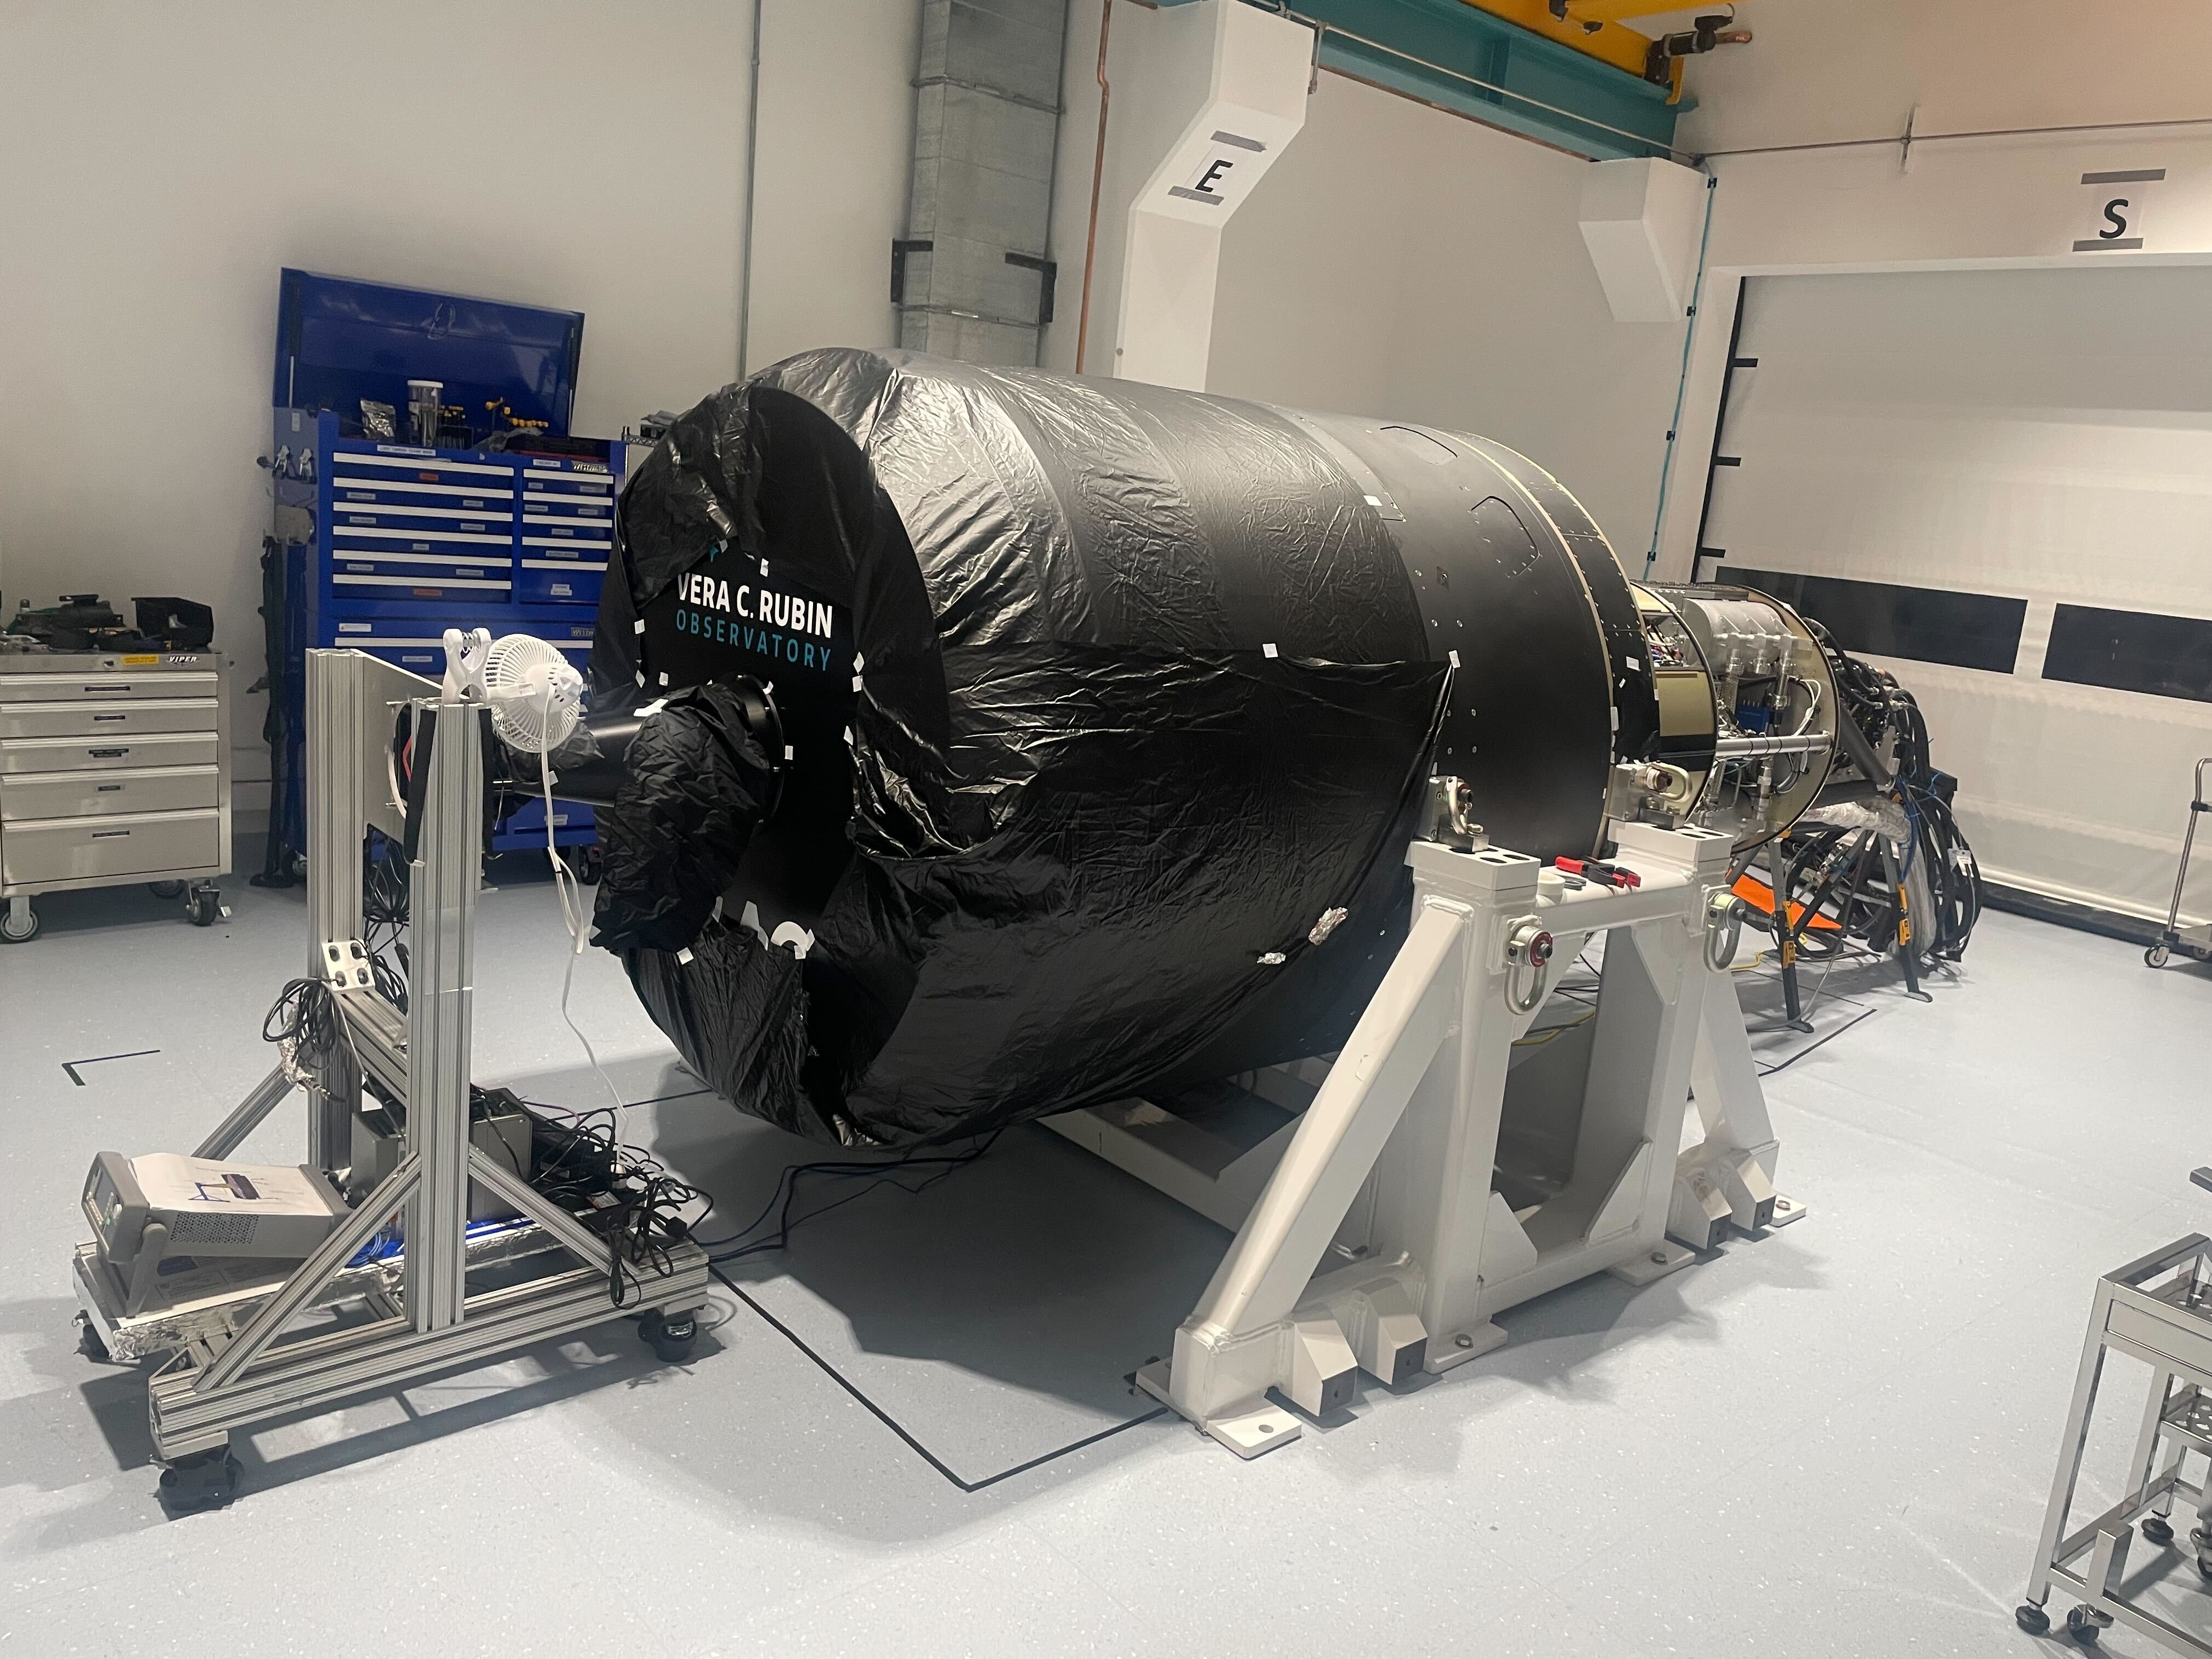
\includegraphics[width=0.6\textwidth]{sections/figures/Camera_Shroud.jpg} 
    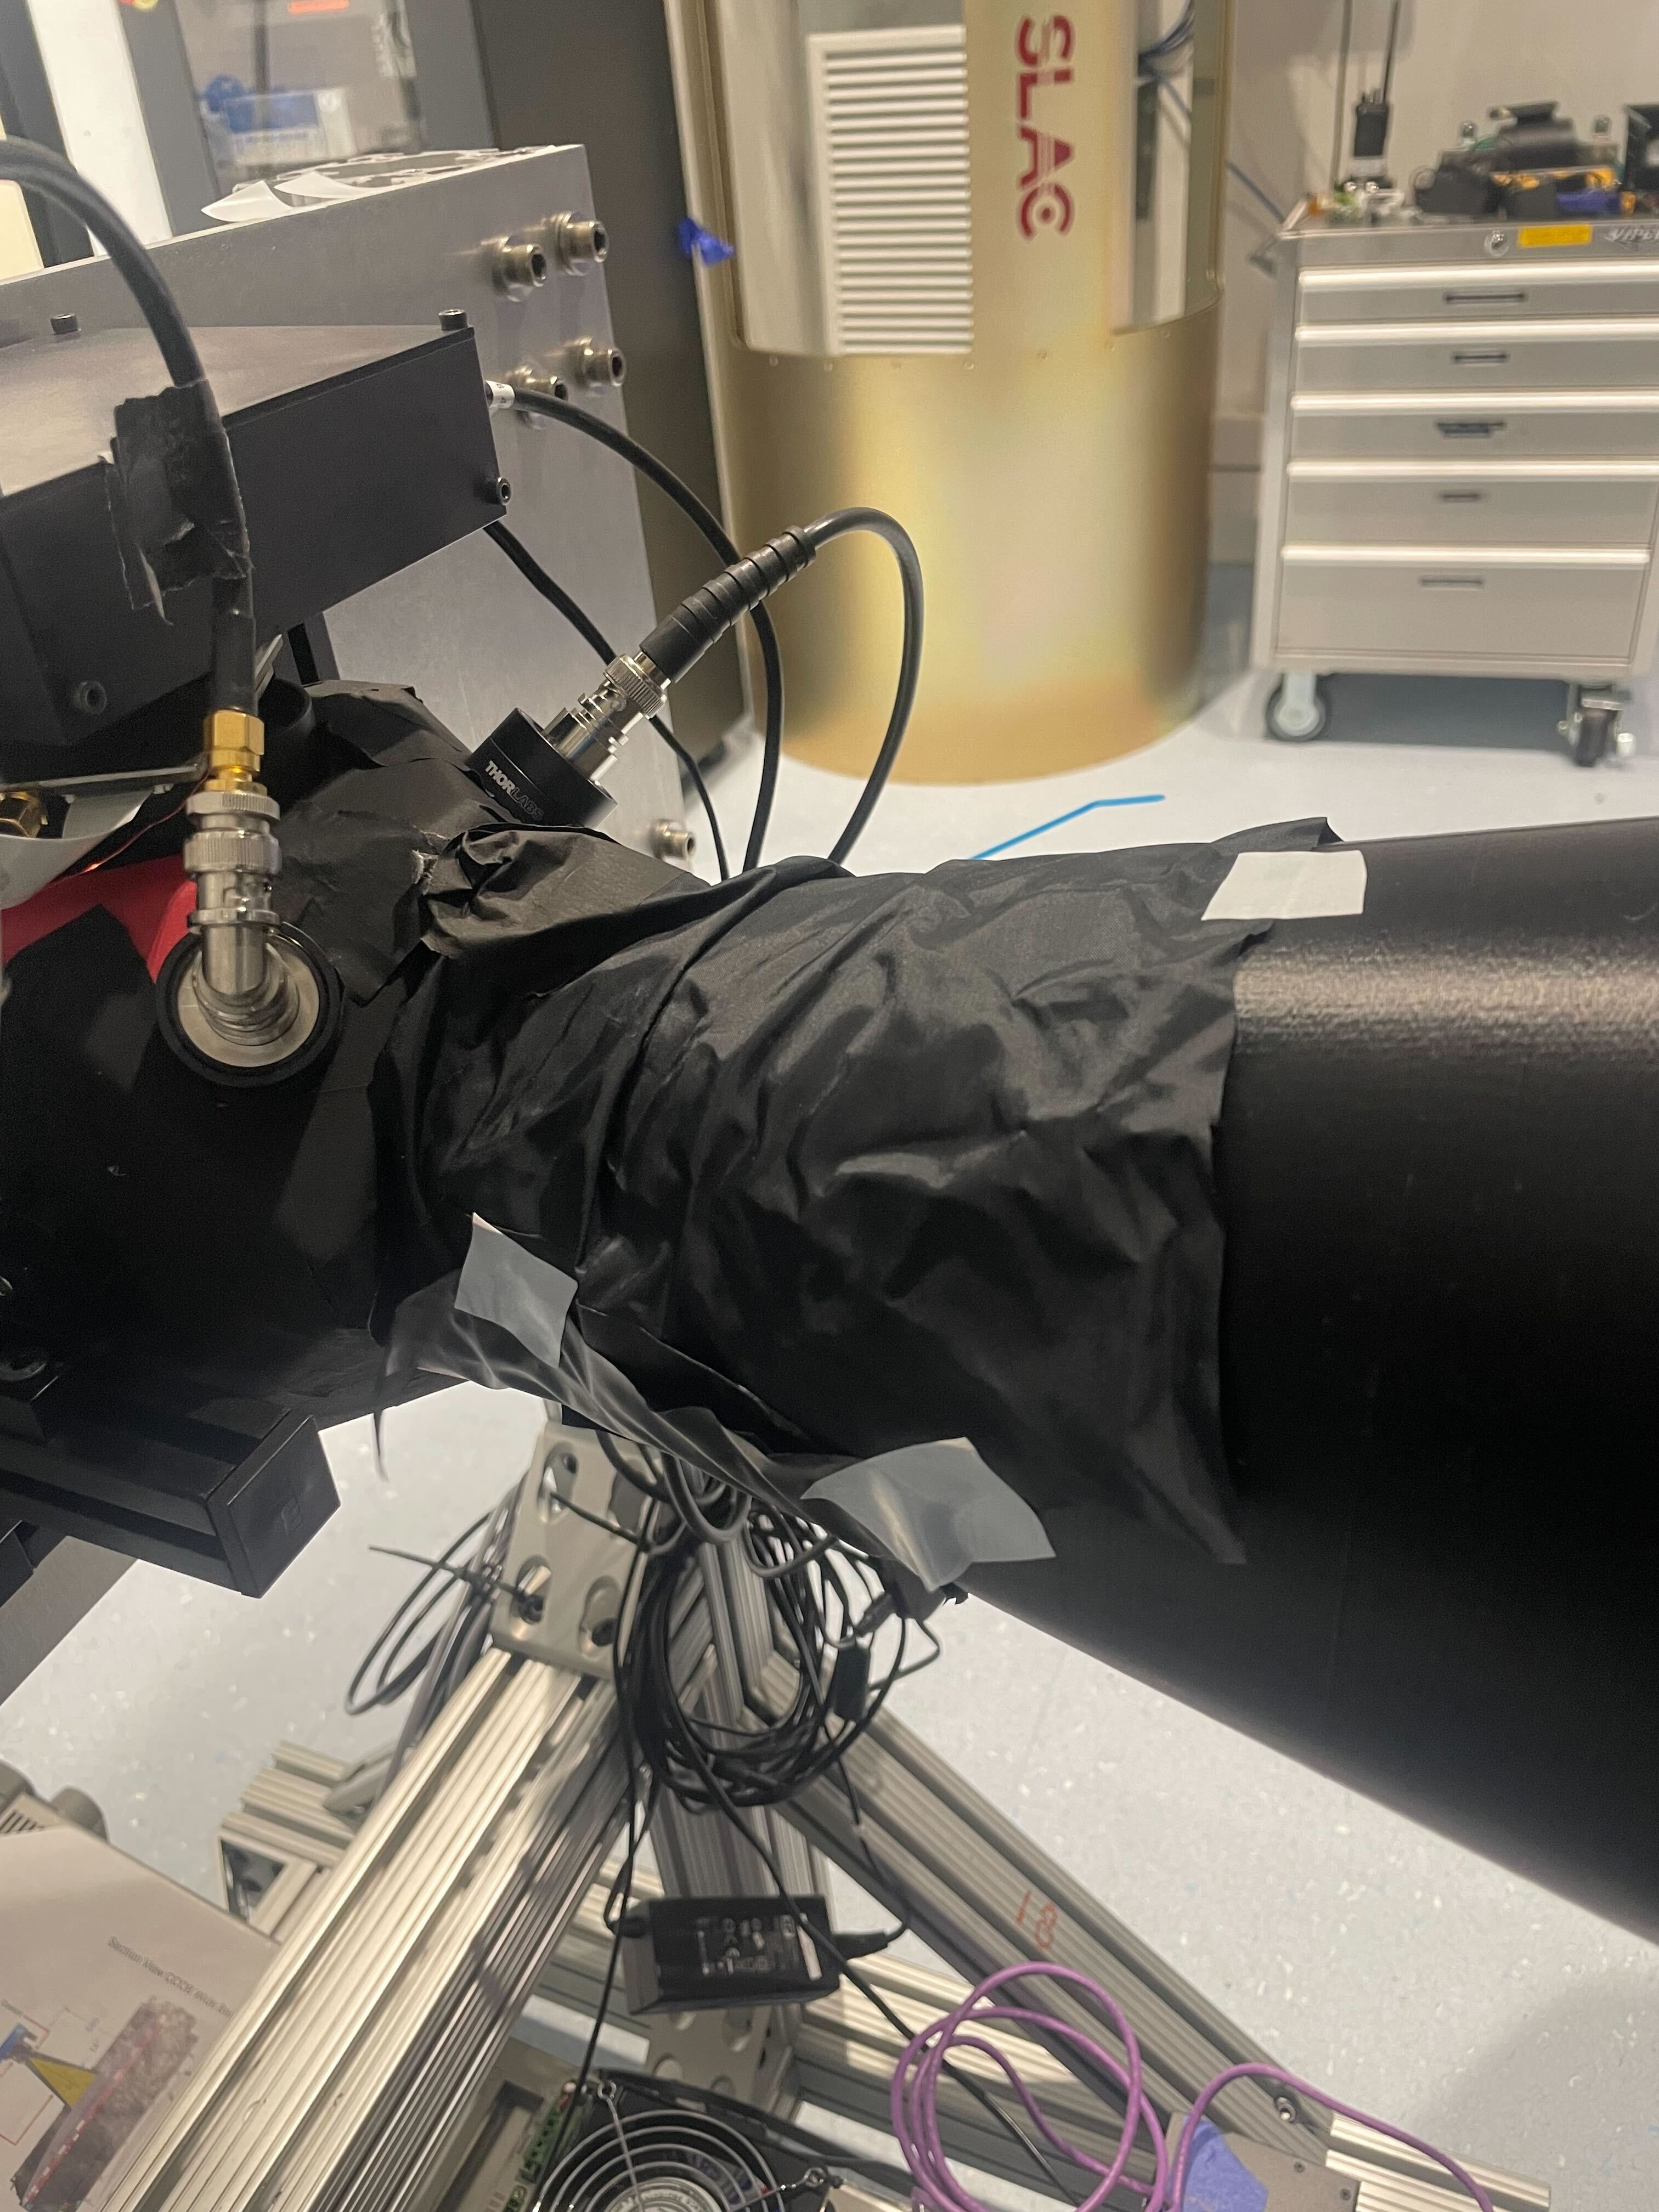
\includegraphics[width=0.35\textwidth]{sections/figures/CCOB_Wide_Shroud.jpg} \\

\caption{(left) Final shroud configuration of LSSTCam in Level 3 to reduce light leaks. (right) CCOB Wide Beam attached to the cone and shrouded.}
\label{fig:LSSTCam_config}
\end{figure}

This allowed us to operate on Level 3 with a dark current of
\textless0.1 ADU/sec with the shutter open. The initial setup of the
CCOB Wide Beam projector was the same as for Run 6, with a minimal ND filter (10 \%)
attached to a C-mount lens. One difference was that the f/stop of the lens
was changed from 2.6 to 1.6 (fully open). This was done to try to
reduce the effect of the `weather' and
the `CMB pattern' two effects that we
found in Run 6 and were found to be due to our projection setup (see
\hyperref[Banovetz2024]{{[}Banovetz2024{]}}). While changing  the f/stop  did
reduce the weather pattern, it also caused a much steeper illumination roll-off
across the focal plane. We evaluated the weather pattern and illumination roll-off relative to Run 6.


To both reduce the effect of the
`weather' and
`CMB' but retain uniform illumination
across the focal plane, we installed a diffuser in the cone attached to
L1. Figure~\ref{fig:diffuser} shows the placement of the diffuser within the cone.

\begin{figure}
\centering
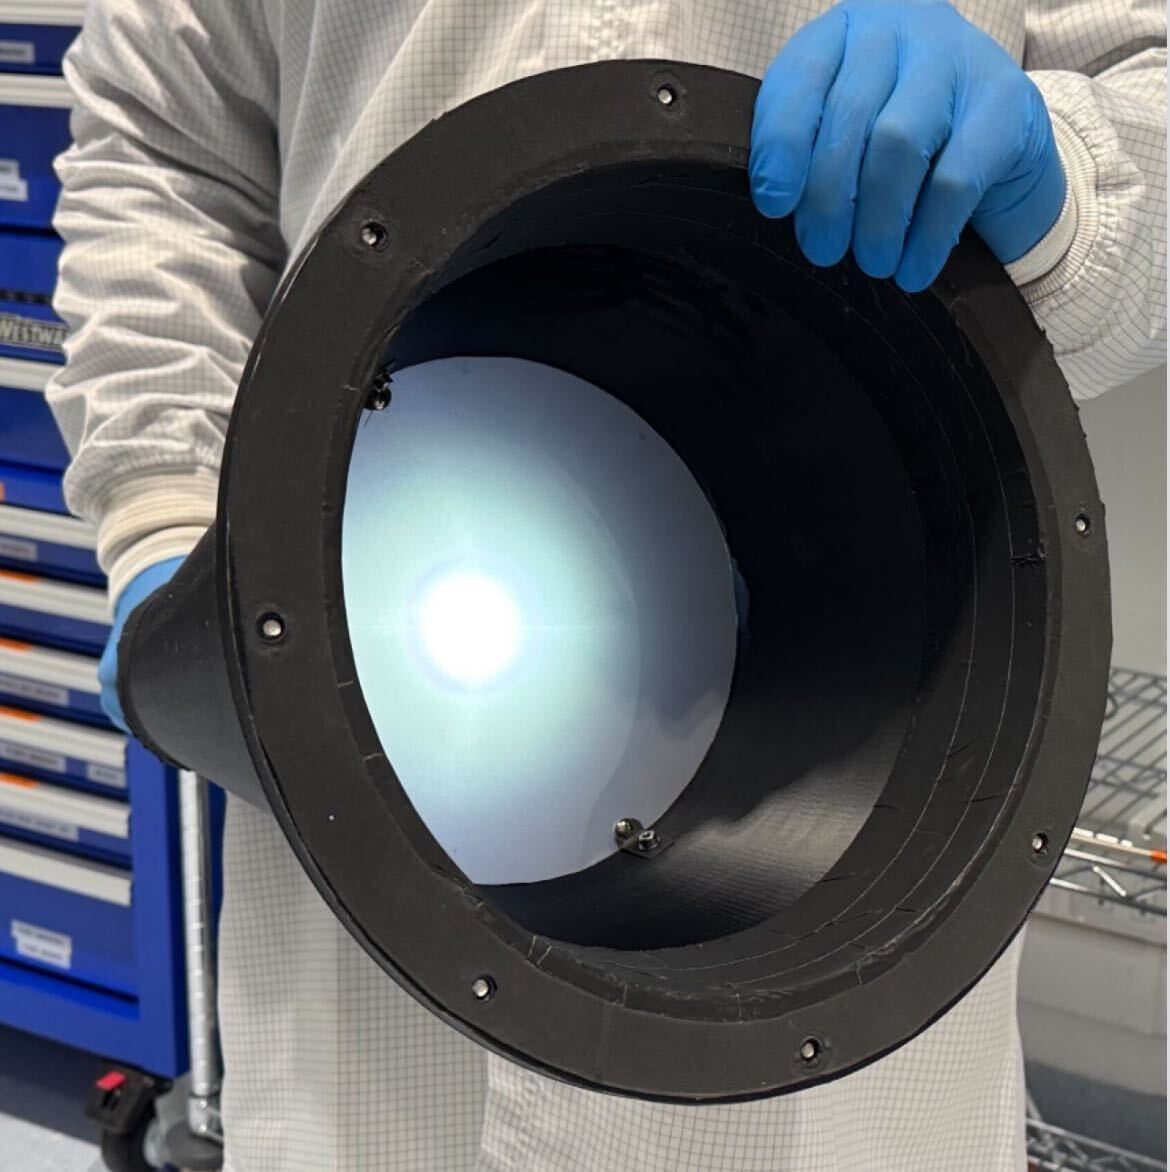
\includegraphics[width=0.9\textwidth]{sections/figures/Diffuser.jpg}
\caption{Diffuser installed into the light cone.}
\label{fig:diffuser}
\end{figure}

The diffuser combined with a fully open f/stop effectively reduced the
incoming light by roughly 35\%. Adjusting for that, we found that it
greatly reduced the `weather' (Fig.~\ref{fig:weather})  and
eliminated the CMB pattern, and more uniformly illuminated the focal
plane  (Fig.~\ref{fig:roll-off}). 

\begin{figure}[htbp]
\centering
\begin{minipage}{0.45\textwidth}
    \centering
    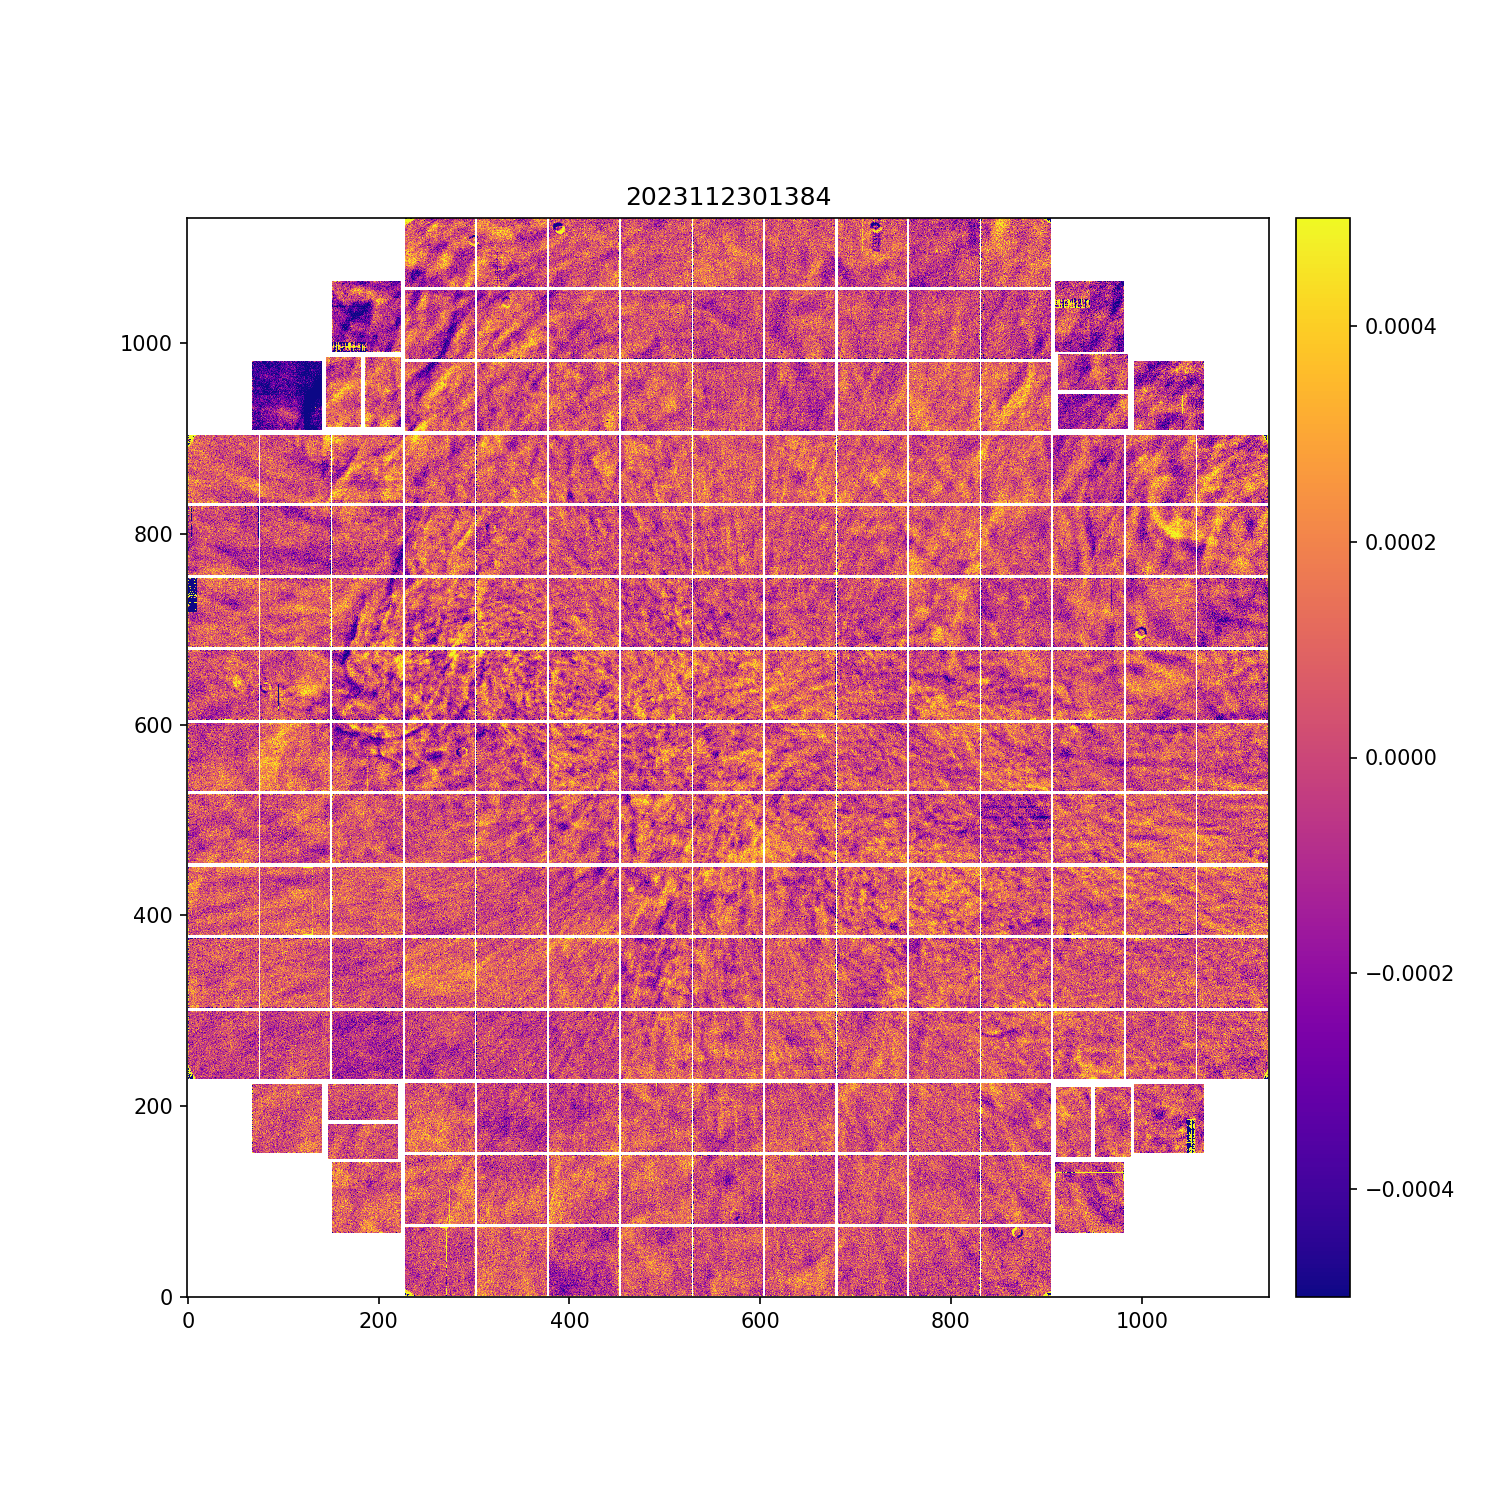
\includegraphics[width=\linewidth]{sections/figures/Run6_Weather.png}
%    \caption{Full focal plane image showing the fractional difference in Run 6.}
\end{minipage}
%\hfill
\begin{minipage}{0.5\textwidth}
    \centering
    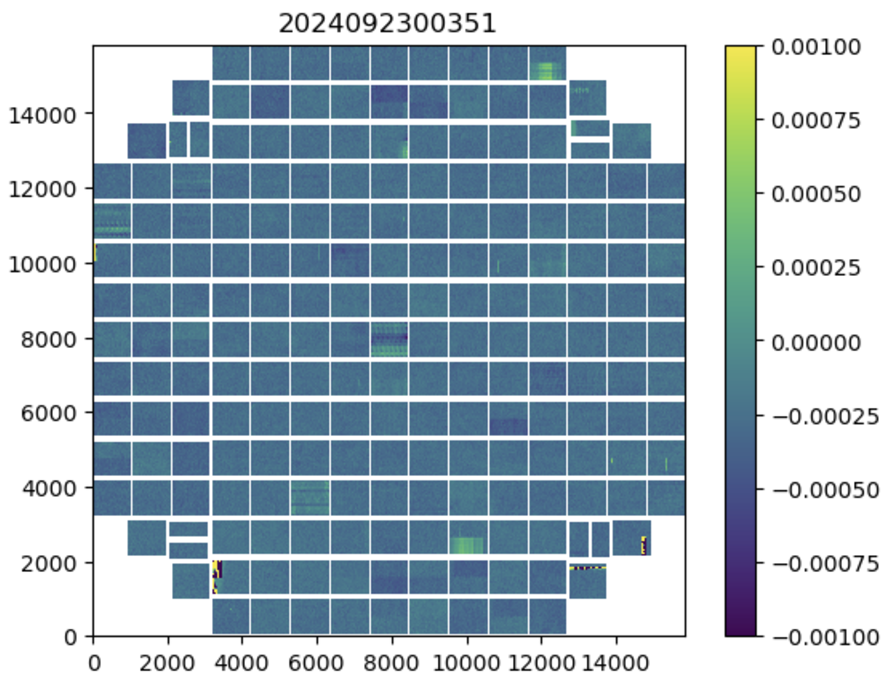
\includegraphics[width=\linewidth]{sections/figures/Run7_WeatherDiffuser.png}
\end{minipage}    
    \caption{Full focal plane fractional difference images for Run 6 (left) and Run 7 (right).}

\label{fig:weather}
\end{figure}

\begin{figure}[htbp]
\centering
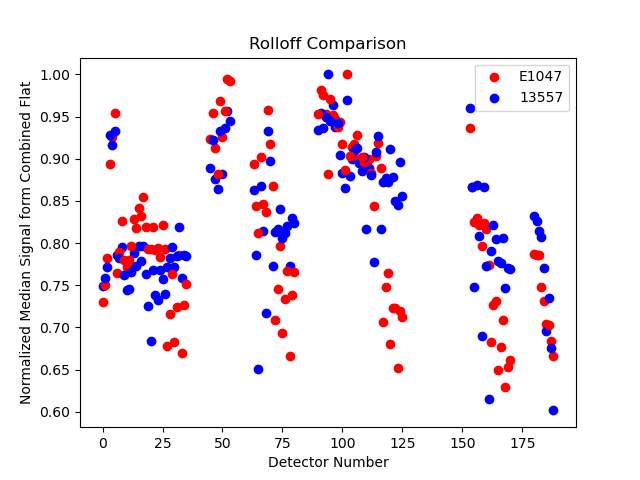
\includegraphics[width=0.9\textwidth]{sections/figures/Run7_DiffuserIllumination.png}
\caption{Illumination across the focal plane from Run 7 with the diffuser as compared to Run 6.}
\label{fig:roll-off}
\end{figure}

The diffuser was installed for all B protocol and PTC runs moving
forward, being taken out only for pinhole projection runs and when using the
4K projector.

The addition to the projectors used for EO testing was a 4K
projector, similar to those used in conference rooms. This projector was
first tested at SLAC and arrived at the observatory about halfway through Run 7.
It was used primarily as a spot projector, as the pinhole filter
was not operational but more importantly, it could
illuminate all 3206 amplifiers instead of the 21 illuminated by the
pinhole projector. Most runs included the spots and the spot fluxes were
controlled by the LSSTCam shutter instead of any flashing (e.g., CCOB Wide Beam). One
downside that was found was that the projector illuminated the entire focal plane at some background level, not just the spot regions. The background illumination also had
structure that changed with time and could not be easily subtracted. The resulting contrast between the spot and the background was only about a factor of 6. Changing the spot shape to large rectangles for crosstalk
measurements increased the contrast ratio to 30.

\subsection{Projector spots}\label{projector-spots}

This section describes the spots and rectangle patterns used for tests with the 4k
projector.

\begin{itemize}
\tightlist
\item
  Projector background
\item
  Spots on many amps
\item
  Spots on one amp
\item
  Optical setup
\end{itemize}

\subsection{Dark current and light
leaks}\label{dark-current-and-light-leaks}

This section describes dark current and light leaks in Run 7 testing.

\subsubsection{Light leak mitigation with shrouding the camera
body}\label{light-leak-mitigation-with-shrouding-the-camera-body}

One of the first tests we attempted with LSSTCam was measuring dark
current and sources of light leaks in the camera body. Before beginning we covered gaps between the L1 cover and the gaskets with tape, in locations where we felt comfortable applying it. Below shows the gaps that
we could see between L1 and its cover.

Once these were sealed, we took some initial measurements and then
started to cover the LSSTCam body with a shroud of .... Figure~\ref{fig:shroud} shows the final shroud configuration covering the
camera.
We also found light leaks
where the light cone attached to L1 was housed, and from the Utility
Trunk. 


\begin{figure}
\centering
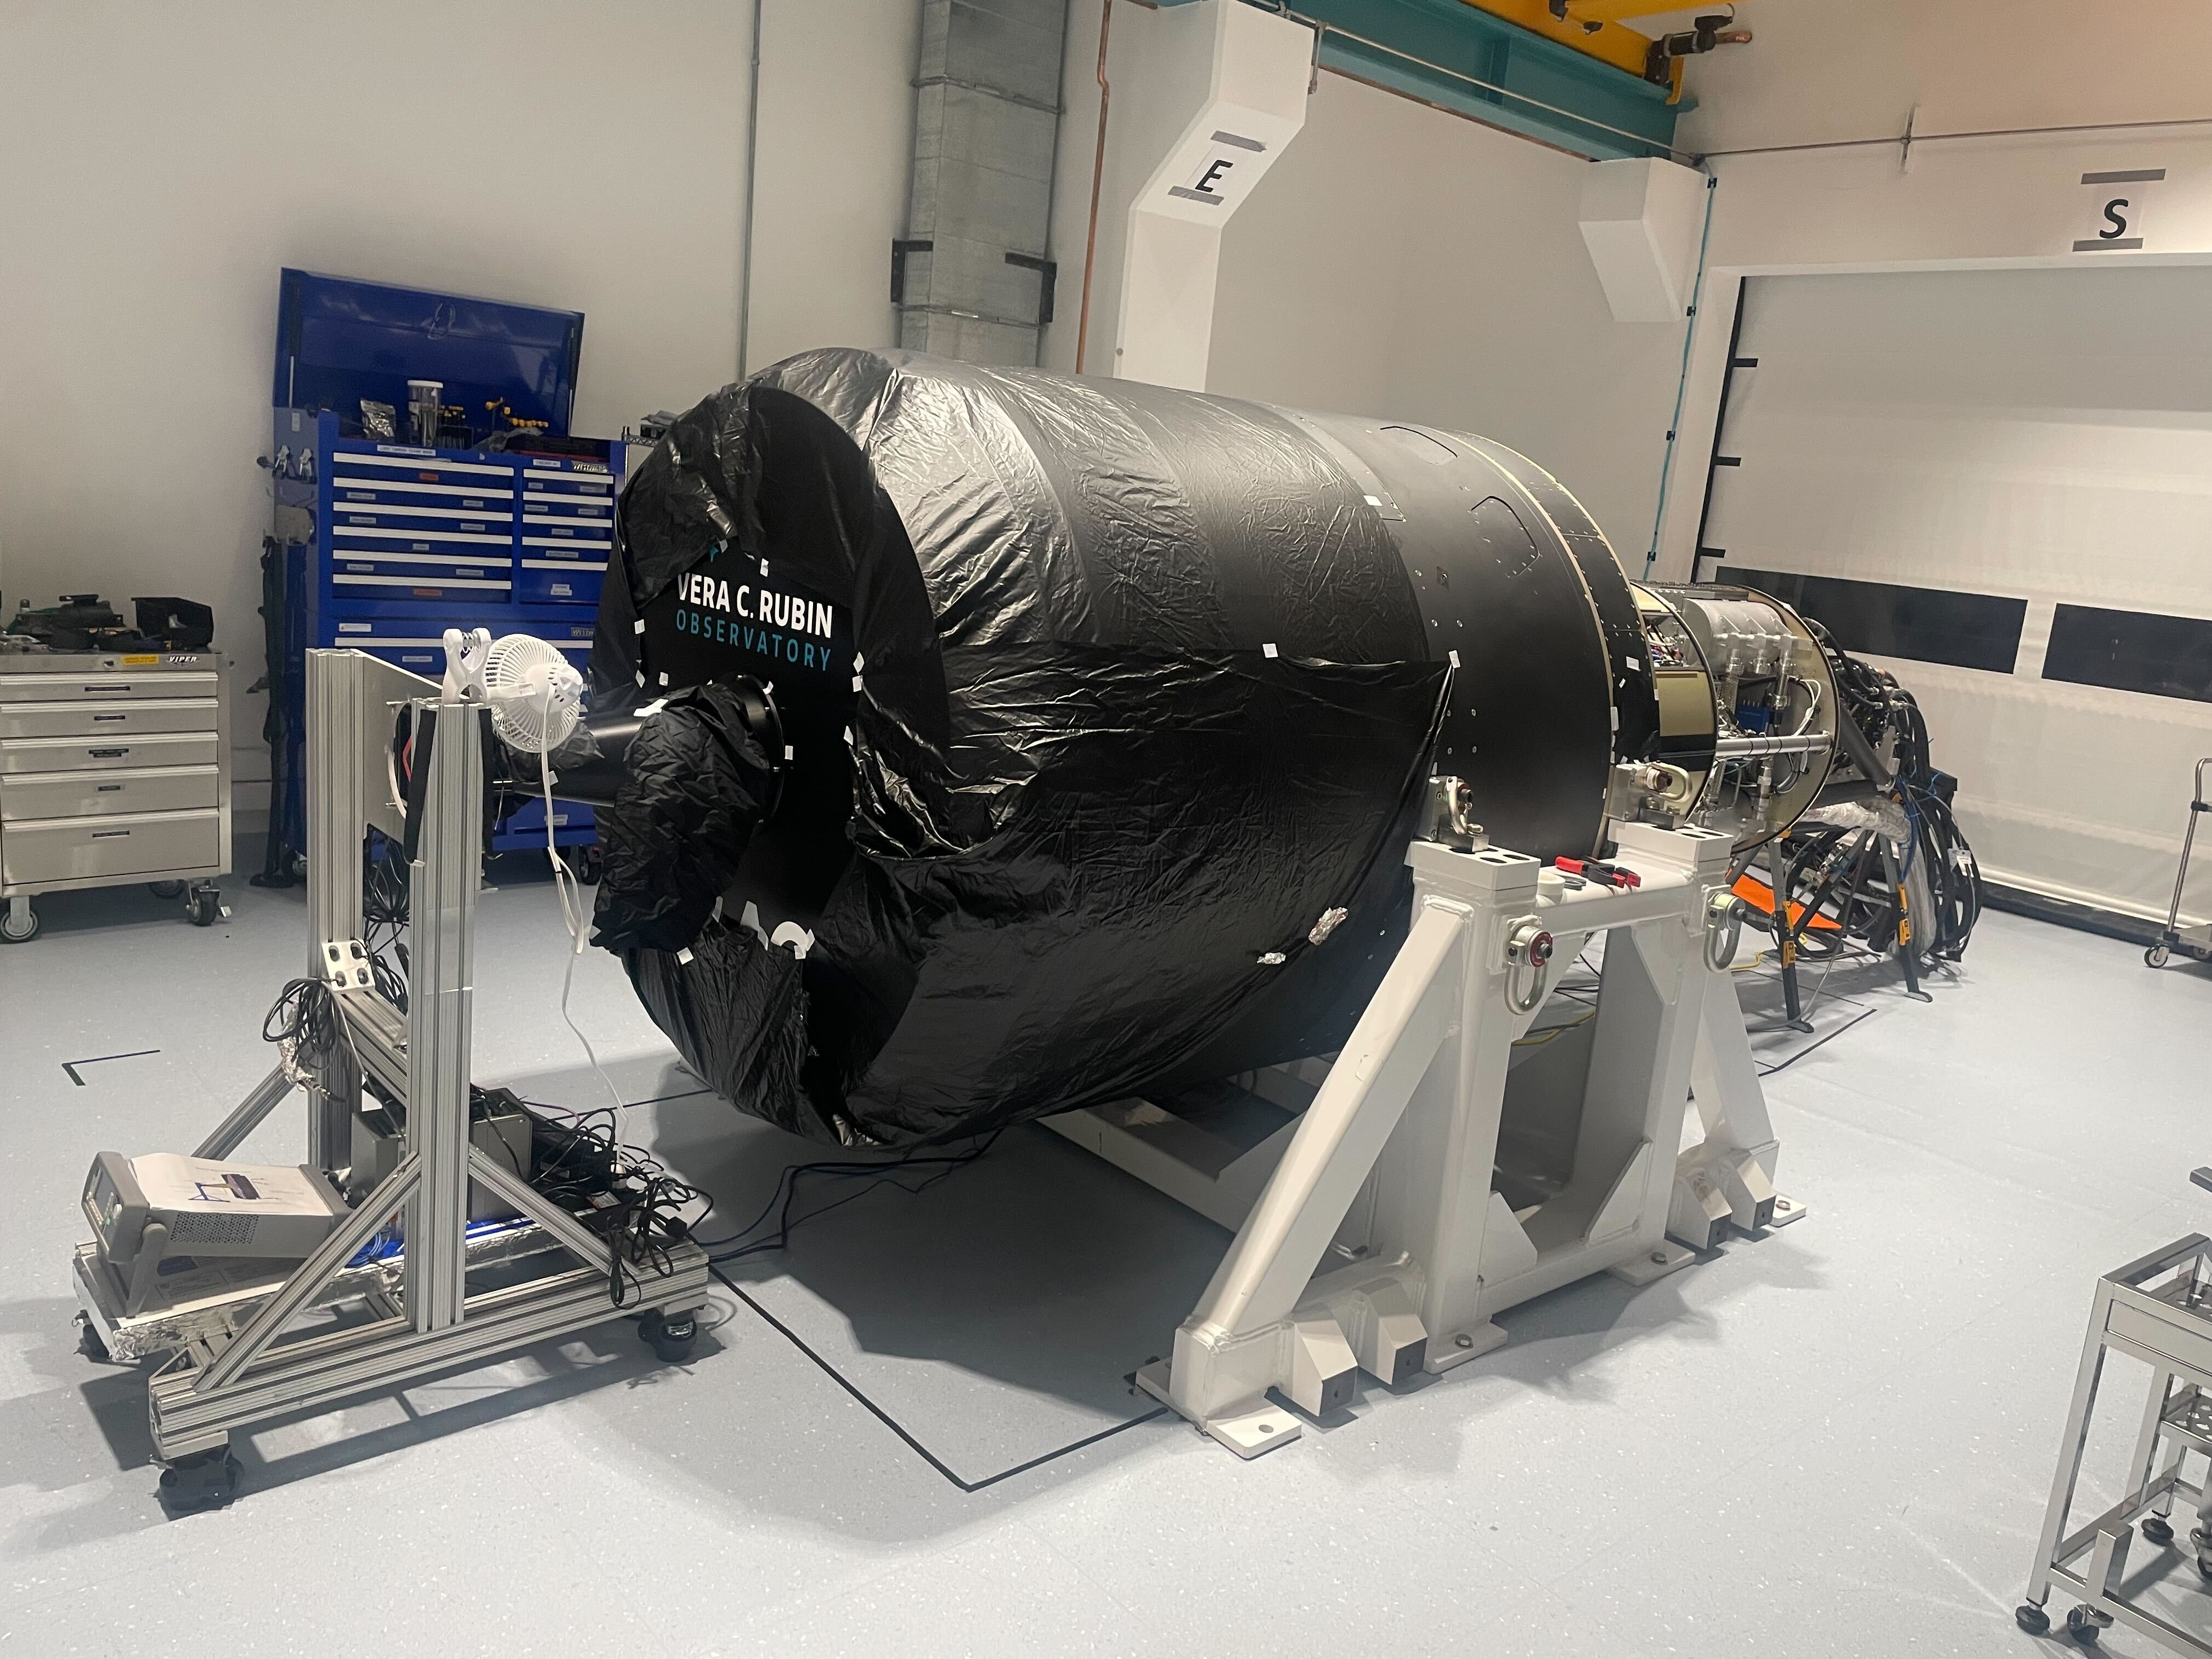
\includegraphics[width=0.9\textwidth]{sections/figures/Camera_Shroud.jpg}
\caption{Final shroud configuration of LSSTCam in Level 3 to reduce
light leaks.}
\label{fig:shroud}
\end{figure}

Table~\ref{tab:leak_chasing} includes the observations, the corresponding measured dark
currents, and comments on what changed during the leak chasing.

\begin{longtable}{|l|c|l|l|l|}
\caption{Summary of the 15\,s dark exposures, the different conditions, and the resulting dark current.
Exposure ID is preceded by ``MC\_C202409".  The shroud was in place for each of these measurements.  (``Initial Covering" was just the CCOB cone and around the L1 cover.) \label{tab:leak_chasing}} \\
\hline
\textbf{Exposure} & \textbf{Dark Current} & \textbf{Room Lights} &\textbf{Shutter} & \textbf{Comments} \\

\hline
\endfirsthead
\hline
%\textbf{Exposure ID} & \textbf{Dark Current (e$^-$/s)} & \textbf{Room Lights} & \textbf{Shutter} & \textbf{Comments} \\
\hline
\endhead
\hline
\endfoot
\hline
09\_000012 & 0.158 & Off & Closed & \\
09\_000018 & 0.158 & On & Closed & \\
09\_000038 & 2.94 & On & Open & Initial Covering  \\
09\_000054 & 1.34 & On & Open &  + Blanket over the FCS \\
09\_000072 & 0.41 & On & Open &  + Blanket over AND under the FCS \\
09\_000078 & 0.18 & Off & Open & + Blanket over AND under the FCS \\
10\_000031 & 0.033 & On & Open &  + Blanket over AND under the FCS + UT \\

\end{longtable}


\subsubsection{Filter Exchange System Autochanger light leak
masking}\label{successful-autochanger-light-leaks-masking}

A dedicated light leak study of the Filter Exchange System (FES) Autochanger (AC) was performed during Run 6 at SLAC
in summer 2023 and a localized faint light source of up to
\textasciitilde{}0.04 e$^-$/s/pix was found to be associated with the 24\,V Clean of
the AC.

In the AC this voltage is used to power some probes and all
controllers. In February 2024, as AC-1 was extracted from LSSTCam for
global maintenance, a direct investigation to localize the light
source was performed unsuccessfully. A light source in the AC
was not expected, as in the AC all controllers' LEDs have
been removed, and most electronics are in ``black boxes". Still, two small
probes, which had LEDs that could not be removed, were initially masked
by a black epoxy. As we had doubts about the quality of this masking at
IR wavelengths, we applied extra masking (aluminum black tape) on them during
the Feb 2024 maintenance (on AC 1 and 2).

At the start of Run 7 a new study of the light leak based on 900\,s
dark exposures with the shutter open and the empty frame filter in
place, showed that the AC light leaks were still present (see left hand image of Fig.~\ref{fig:ac-light-leak}). Following this finding, a full review of all the AC hardware powered
by the 24 V dirty was performed, and a candidate was found: the encoders
of the five main motors of the AC had only partial documentation from the
vendor that did not mention the presence of LEDs. After interaction with the
vendor, the encoders were understood to contain \textasciitilde700\,nm LEDs. The hypothesis of \textasciitilde700\,nm LED sources has been
found compatible with the observation as no AC light leaks were detected
using various filters (g, r, and y) in LSSTCam at the start of Run 7 (g, r, and y
filters). A dedicated test in Paris using an AC spare encoder and a
precision photometric set-up allowed identification of the leak in the masking of
those LEDs in the vendor packaging. A complementary masking method based
on a 3D printed part + tape + cable tie was qualified in Paris.  It was
found to mask the light leak and to be safe (all parts correctly secured).

In November 2024, we masked all the lights in the back of the Level 3 white
room (not the part containing LSSTCam) to set up a high-quality dark room
allowing a direct observation with a CMOS camera of the light leak on
the AC2 motor encoders. The level of darkness reached allowed us to
validate the quality of the light masking of the AC encoders. Notice that the
FES-prototype in Paris does not have encoders on the Online
Clamps, so we had to tune/qualify the masking of those encoders directly on the AC 2 at the summit.

For both AC 1 and 2, the encoders of the five motors with the vendor issue on
their LED masking have been successfully enveloped in a light-tight
mask.

We note that the AC was turned off starting on 27 September 2024 at 21:15 UTC in the
first part of Run 7. For the second part of Run 7 (i.e., after
mid-November) the AC was back on: as the AC 1 was back in LSSTCam with
the new light masks in place on the motor encorders, we were able to take a new series of
900\,s darks with the AC turned on and off, confirming that the light leak
associated with the FES was eliminated (see right hand image of Fig.~\ref{fig:ac-light-leak}).

\begin{figure}
\begin{centering}
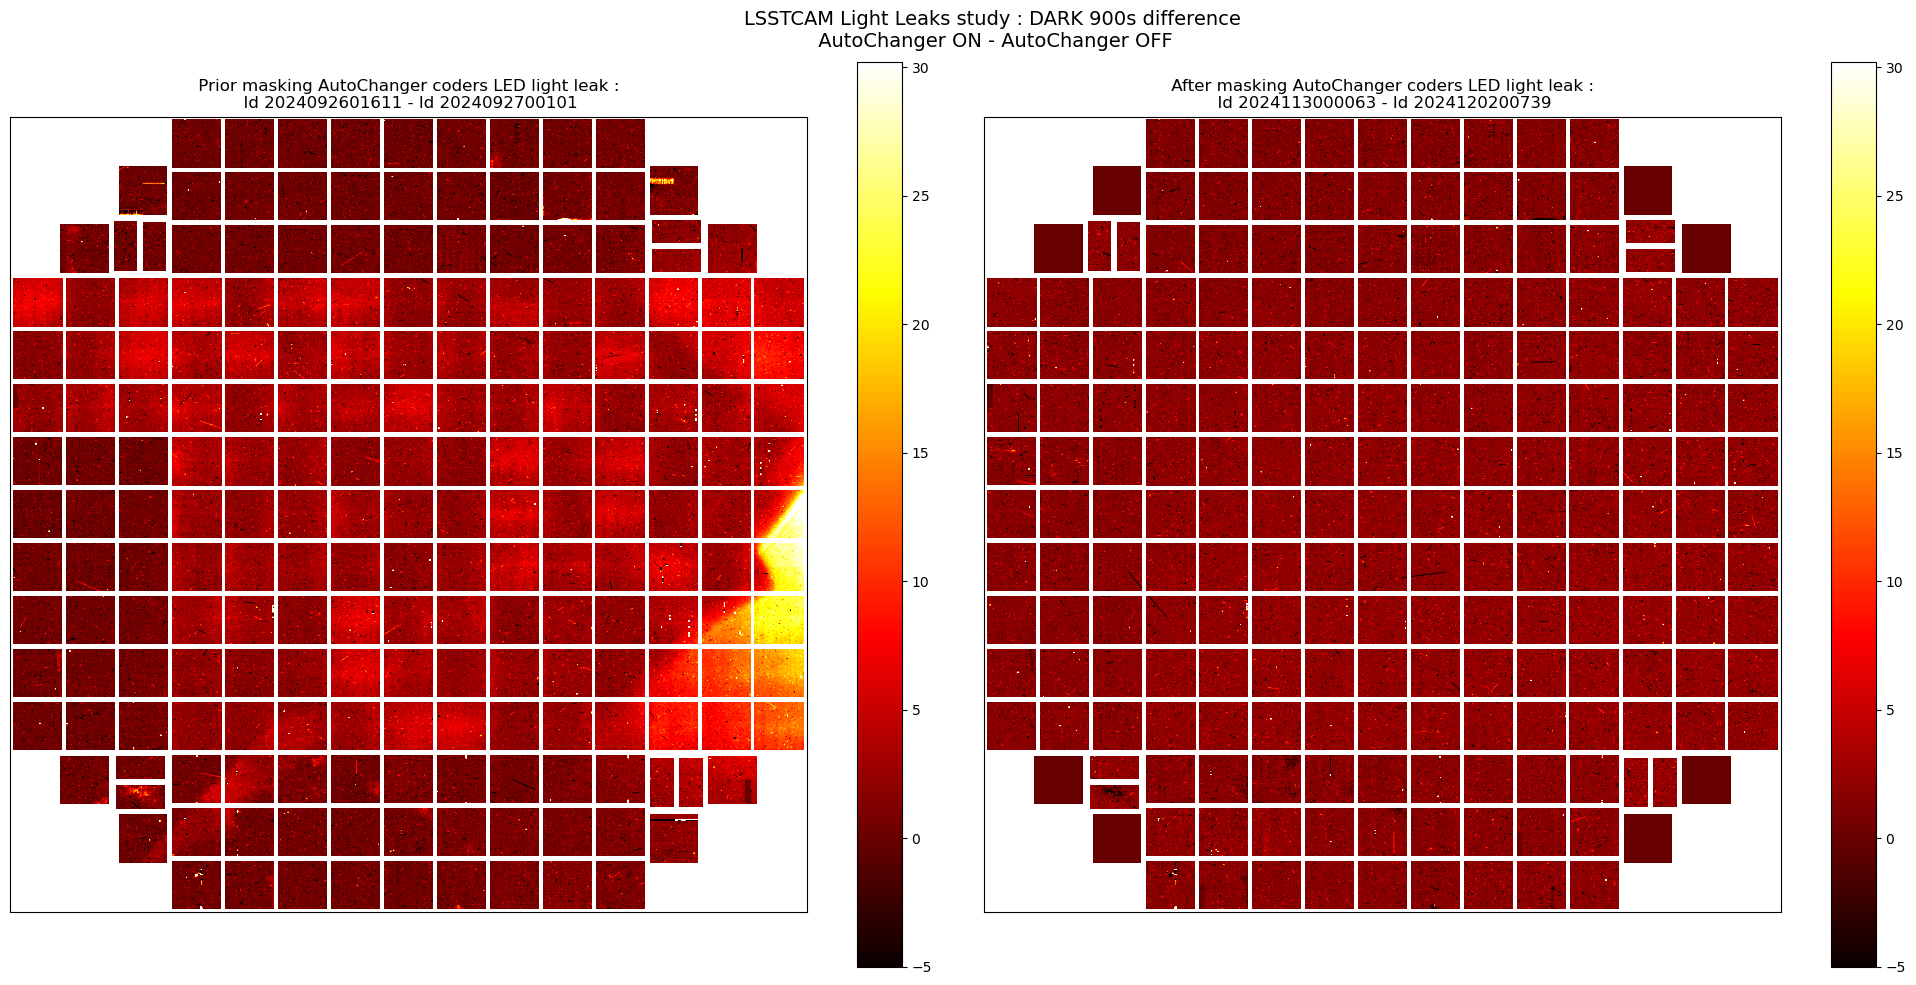
\includegraphics[width=0.8\textwidth]{sections/figures/AC_LightLeak_study.png}
\caption{ (left) The original impact of the AC light leak on a 900\,s dark difference image (AC on minus AC off). (right) The result after masking the LEDsc of the motor encoders in the AC.  No light associated with the FES is present in 900\,s dark difference image.  \label{fig:ac-light-leak}}
\end{centering}
\end{figure}

\paragraph{Shutter condition impact on
darks}\label{shutter-condition-impact-on-darks}

\paragraph{Filter condition impact on
darks}\label{filter-condition-impact-on-darks}

\subsubsection{Final measurements of dark
current}\label{final-measurements-of-dark-current}

\section{Reverification}\label{reverification}

All electro-optical (EO) camera test data is processed through the
\underline{\href{https://github.com/lsst/cp_pipe/tree/main}{calibration products}} and
\underline{\href{https://github.com/lsst-camera-dh/eo_pipe/tree/main}{electro-optical}}
pipelines to extract key metrics from the data run. The key camera
metrics from Run 7, and their comparison to previous runs are discussed
below.

The naming of the EO runs was established during initial LSSTCam
integration and testing. The final SLAC IR2 run from November 2023 was
named ``Run 6", while the data acquisitions from Cerro Pachon beginning in October 2024 are
considered ``Run 7." Additionally, individual EO acquisitions are tagged
with a run identifier. This is commonly referred to as a Run ID. For all
SLAC runs, the run identifier was a five digit numeric code, while the
Cerro Pachon runs were ``E-numbers" that started with a capital E
followed by a numeric code.

Among the motivations for these measurements, the primary concern is whether LSSTCam has
maintained its performance characteristics between Run 6 and Run 7.

\subsection{Background}\label{background}

Initial characterization studies performed on LSSTCam during Run 7 primarily used two
image acquisition sequences.

\begin{itemize}
\tightlist
\item
  B protocols: this acquisition sequence consists of the minimal set of
  camera acquisitions for electro-optical testing, including

  \begin{itemize}
  \tightlist
  \item
    Bias images
  \item
    Dark images
  \item
    Flat pairs - flat illumination images (flats) taken at varying flux levels
  \item
    Stability flats - flats taken at constant flux levels
  \item
    Wavelength flats - flats taken with different LEDs
  \item
    A persistence dataset - a saturated flat, followed by several darks
  \end{itemize}
\item
  PTCs (photon transfer curves): this acquisition sequence consists of a
  sequence of flat pairs taken at different flux levels. The flat
  acquisition sequence samples different flux levels at a higher density
  than the B protocol flat sequence, enabling more precise estimates of
  flat pair metrics including pixel covariances (see Fig. \ref{fig:PTC_BProtocol_Comparison}).
\end{itemize}

\begin{figure}[H]
\begin{centering}
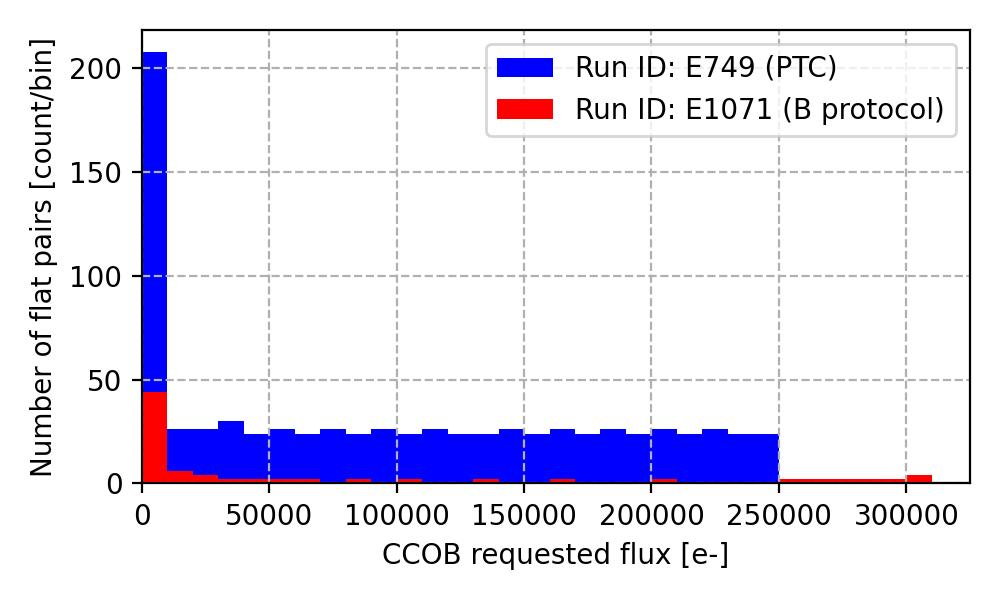
\includegraphics[width=0.7\textwidth]{sections/figures/baselineCharacterization/PTC_BProtocol_Comparison.jpg}
	\caption{Flat-pair comparison between PTC and B protocol
\label{fig:PTC_BProtocol_Comparison}}
\end{centering}
\end{figure}

For comparisons between Cerro Pachon EO runs and the final SLAC IR2 equivalents, the following runs are used (see Table~\ref{runTable-b-ptc}).

\begin{longtable}[H]{@{}
  >{\raggedright\arraybackslash}p{(\linewidth - 4\tabcolsep) * \real{0.1806}}
  >{\raggedright\arraybackslash}p{(\linewidth - 4\tabcolsep) * \real{0.2083}}
  >{\raggedright\arraybackslash}p{(\linewidth - 4\tabcolsep) * \real{0.2639}}@{}}
\toprule\noalign{}
\label{runTable-b-ptc}
\begin{minipage}[b]{\linewidth}\raggedright
\begin{quote}
Run Type
\end{quote}
\end{minipage} & \begin{minipage}[b]{\linewidth}\raggedright
%SLAC IR2 Run
Run 6
\end{minipage} & \begin{minipage}[b]{\linewidth}\raggedright
%Cerro Pachón Run
Run 7
\end{minipage} \\
\midrule\noalign{}
\endhead
\bottomrule\noalign{}
\endlastfoot
B Protocol & \begin{minipage}[t]{\linewidth}\raggedright
\begin{quote}
13557
\end{quote}
\end{minipage} & \begin{minipage}[t]{\linewidth}\raggedright
\begin{quote}
E1071
\end{quote}
\end{minipage} \\
\begin{minipage}[t]{\linewidth}\raggedright
\begin{quote}
PTC
\end{quote}
\end{minipage} & \begin{minipage}[t]{\linewidth}\raggedright
\begin{quote}
13591
\end{quote}
\end{minipage} & \begin{minipage}[t]{\linewidth}\raggedright
\begin{quote}
E749
\end{quote}
\end{minipage} \\
\caption{Reference runs for Run 6 and Run 7 comparisons}
\end{longtable}

\subsection{Stability flat metrics}\label{stability-flat-metrics}

\subsubsection{Charge transfer
inefficiency}\label{charge-transfer-inefficiency}

CTI, or charge transfer inefficiency, measures the fraction of charge that fails to transfer from row to row during readout, and appears as trailing charge in the image area. Consequences of high CTI include loss of charge, distorted signals in the direction of parallel transfer, and reduced sensitivity in low light imaging. CTI measurements are made using the EPER method \hyperref[EPER]{{[}EPER{]}}, for which the ratio of the residual charge in the overscan pixels to the total signal charge in the imaging region is evaluated. In the context of LSSTCam, we measure CTI along both the serial and parallel directions.

\paragraph{Serial CTI}\label{serial-cti}

\begin{figure}[H]
\begin{centering}
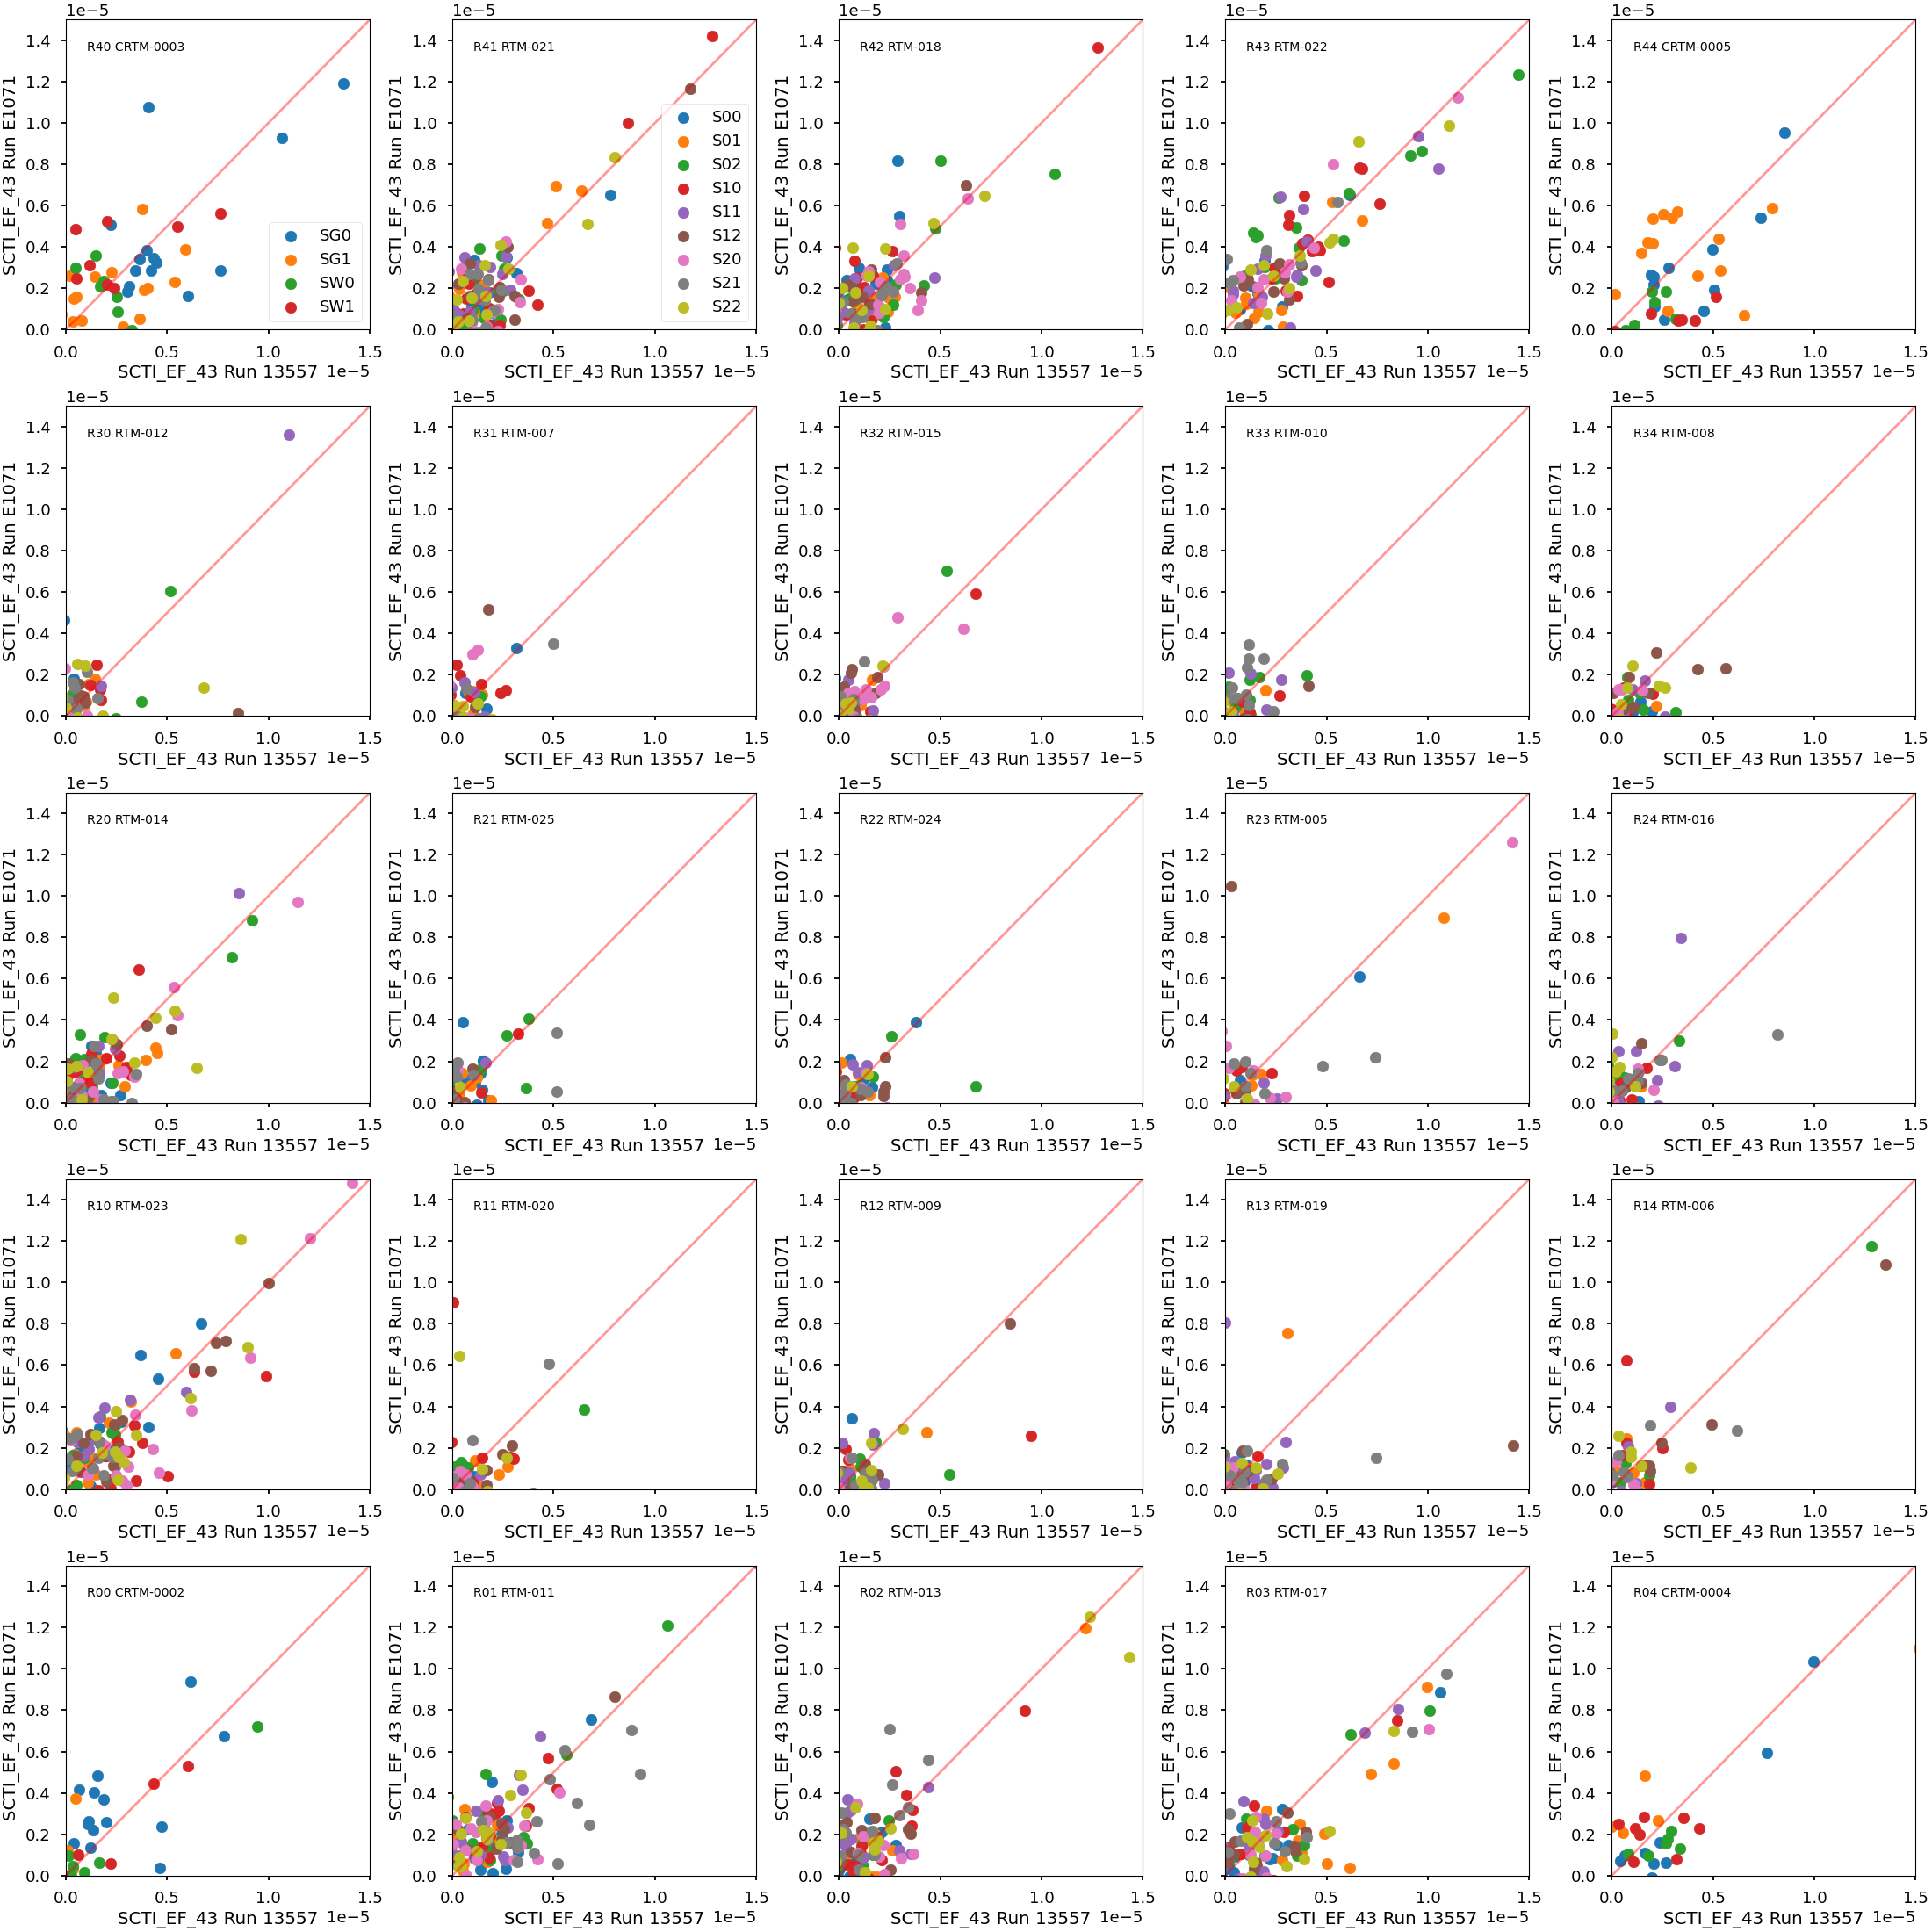
\includegraphics[width=0.7\textwidth]{sections/figures/baselineCharacterization/13557_E1071_SCTI_EF_43.png}
	\caption{Serial CTI comparison by raft for Run 7 (E1017) and Run 6 (13557)\label{fig:serial-cti}}
\end{centering}
\end{figure}

The CTI along the serial registers of the amplifier segments of the LSSTCam CCDs is consistent between Run 6 and
Run 7 (Fig.~\ref{fig:serial-cti}). Both sensor types show extremely low CTI on the order of $10^{-3}$ \%,
and span a range  of \textasciitilde$2 \times 10^{-5}$ \% for e2v sensors, and
by \textasciitilde$4 \times 10^{-6}$  \% for ITL sensors (Fig.~\ref{fig:serial-cti-dist}).

\begin{figure}[H]
\begin{centering}
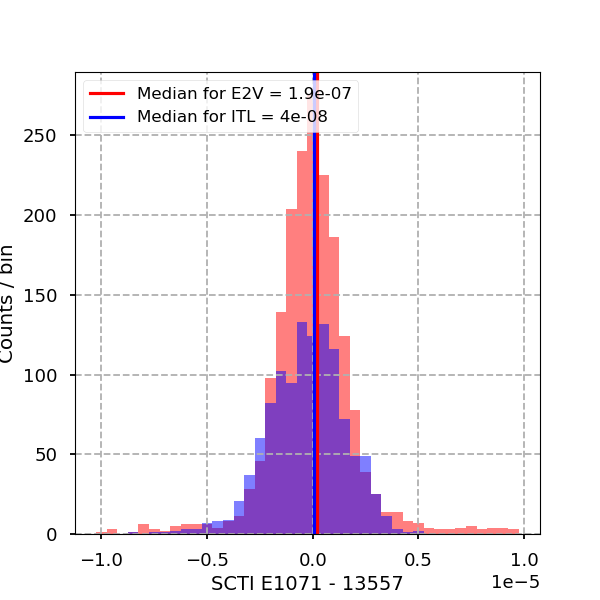
\includegraphics[width=0.7\textwidth]{sections/figures/baselineCharacterization/SCTI_13557_E1071_diff.png}
\caption{Distributions of differences in serial charge transfer inefficiencies between Run 7 (E1071) and Run 6 (13557), grouped by CCD type.}
\label{fig:serial-cti-dist}
\end{centering}
\end{figure}

\paragraph{Parallel CTI}\label{parallel-cti}

The CTI along the parallel direction is consistent between Run 6 and
Run 7 as well (Fig.~\ref{fig:parallel-cti}). Both sensor types are found to have extremely low CTI on the order of $10^{-5}$ \%,
and span a range of \textasciitilde$2 \times 10^{-7}$ \% for e2v sensors, and
by \textasciitilde$7 \times 10^{-6}$ \% for ITL sensors (Fig.~\ref{fig:parallel-cti-dist}).

\begin{figure}[H]
\begin{centering}
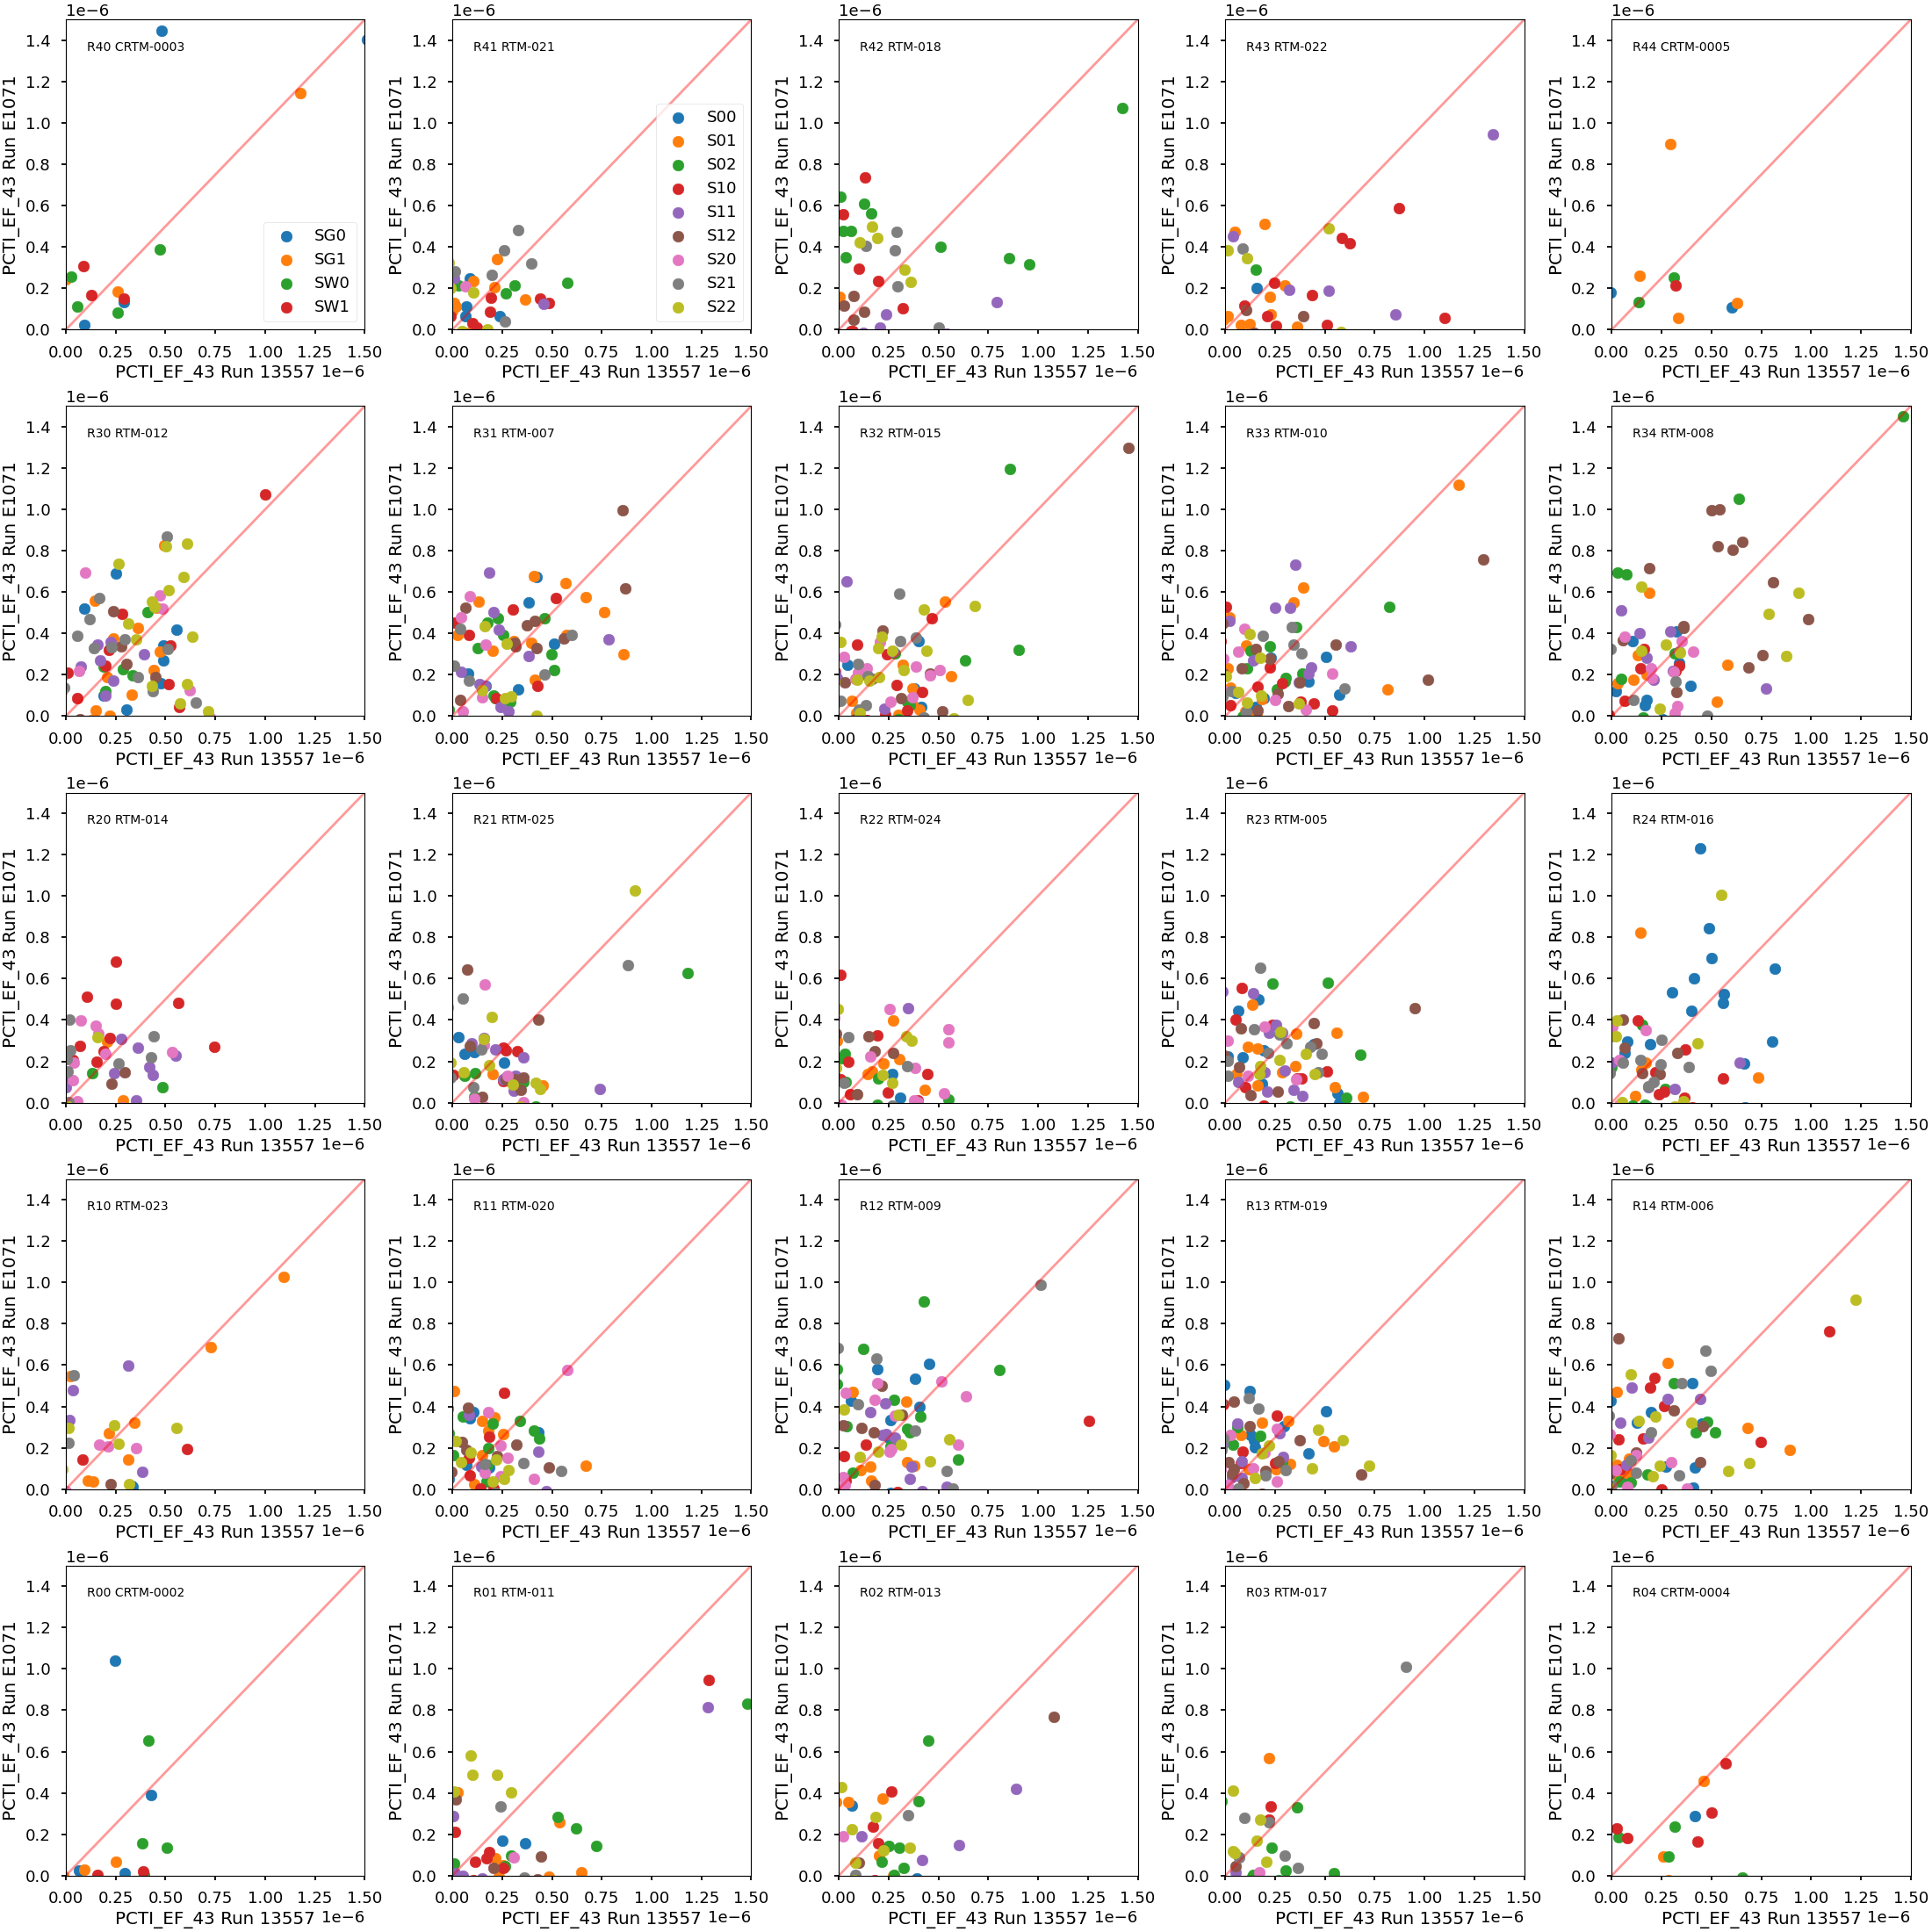
\includegraphics[width=0.7\textwidth]{sections/figures/baselineCharacterization/13557_E1071_PCTI_EF_43.png}
\caption{Parallel CTI comparison by raft for Run 7 (E1017) and Run 6 (13557).}
\label{fig:parallel-cti}
\end{centering}
\end{figure}

\begin{figure}[H]
\begin{centering}
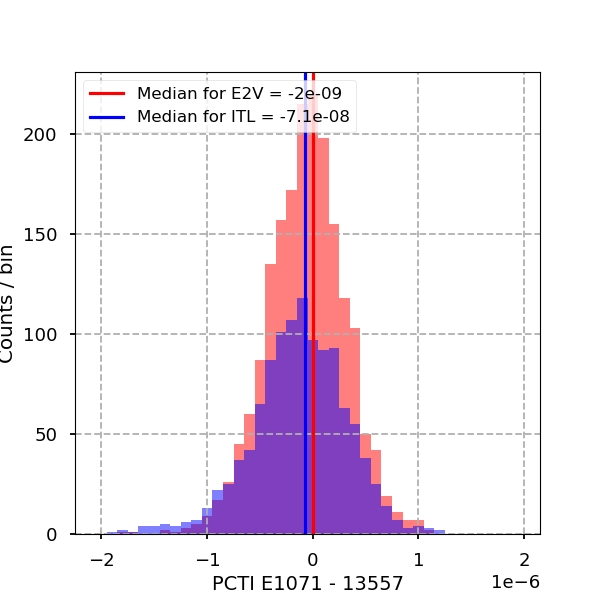
\includegraphics[width=0.7\textwidth]{sections/figures/baselineCharacterization/PCTI_13557_E1071_diff.png}
\caption{Distributions of differences in parallel charge transfer inefficiencies between Run 7 (E1071) and Run 6 (13557), grouped by CCD type.}
\label{fig:parallel-cti}
\end{centering}
\end{figure}

\subsection{Dark metrics}\label{dark-metrics}

\subsubsection{Dark current}\label{dark-current}

Dark current is the small amount of electrical charge generated in the
absence of light due to thermal activity within the semiconductor
material of a CCD. This effect occurs when electron/hole pairs are thermally released
into the conduction band in the CCD, mimicking the signal that light would
produce. Dark current increases with temperature, so cooling the CCD is
a common method to reduce it in sensitive imaging applications. Dark
current introduces noise into an image, degrading its quality,
particularly in low-light conditions or long exposures. In the context
of LSSTCam, we measure dark current from the combined dark images across
all amplifiers.

\begin{figure}[H]
\begin{centering}
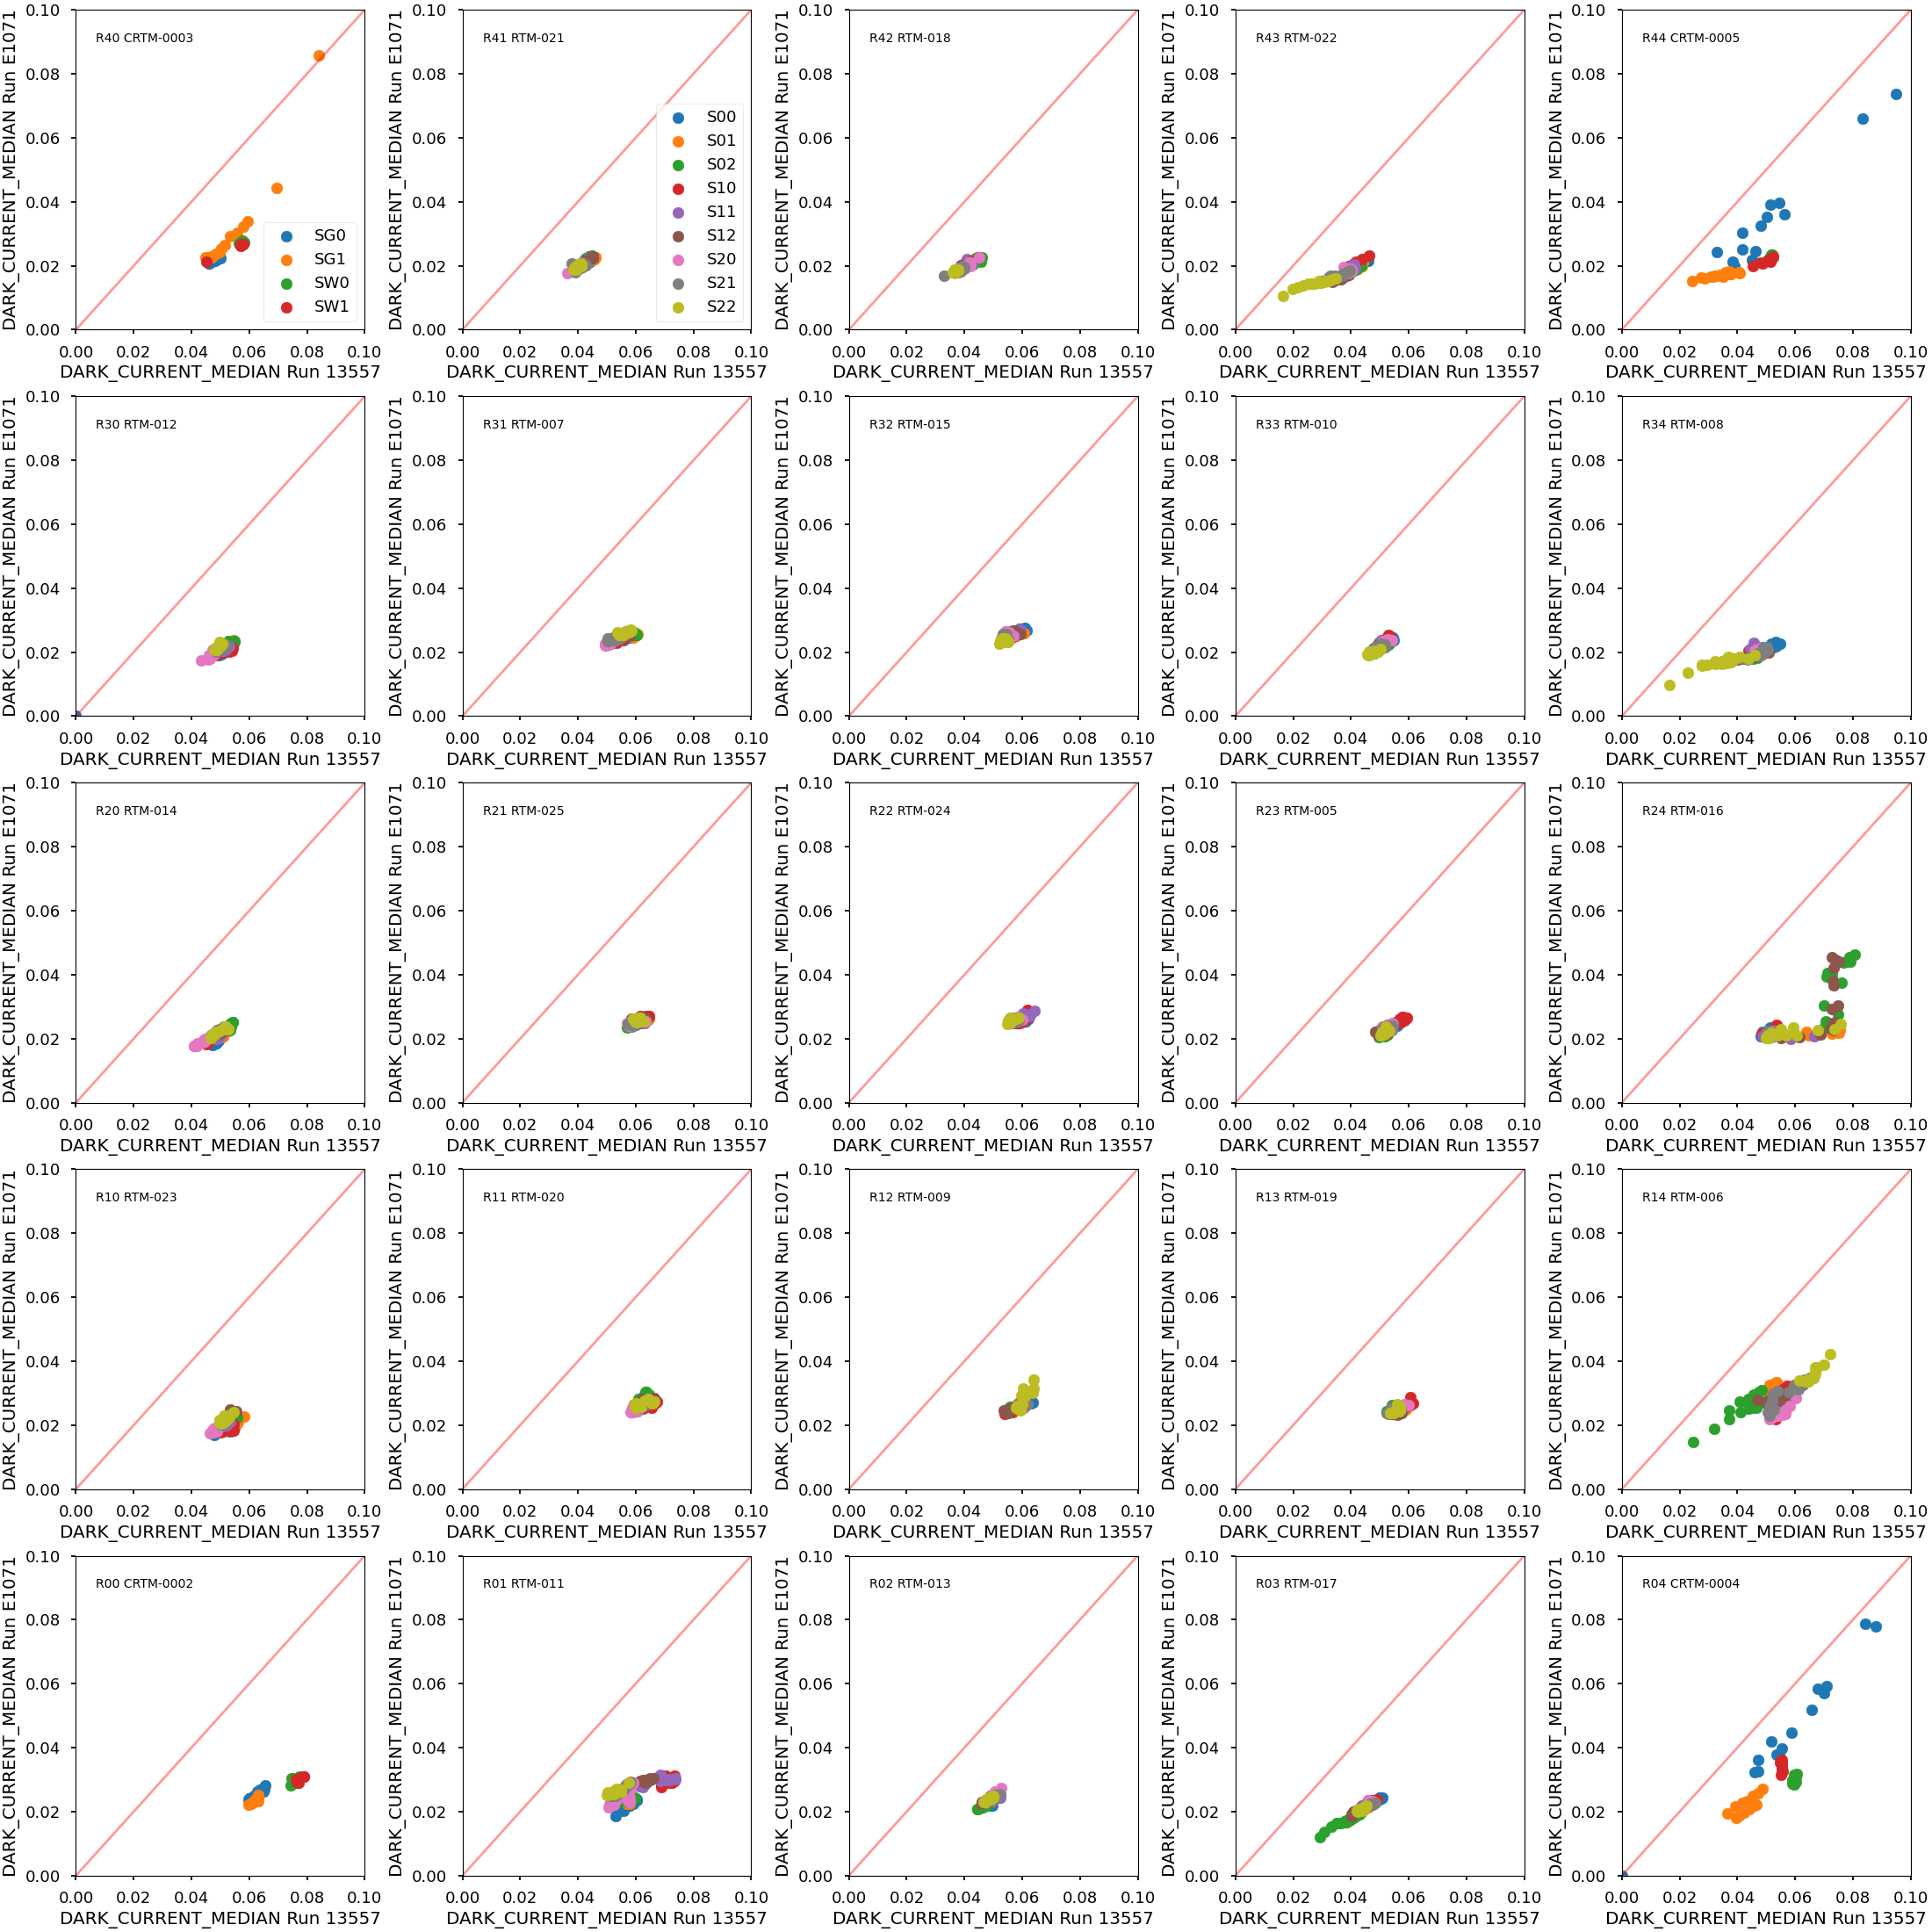
\includegraphics[width=0.7\textwidth]{sections/figures/baselineCharacterization/13557_E1071_DARK_CURRENT_MEDIAN.png}
\caption{Dark current comparison by raft for Run 7 (E1017) and Run 6 (13557).}
\label{fig:dark}
\end{centering}
\end{figure}

Unexpectedly, the dark current was significantly less in Run 7 than
Run 6 (Fig.~\ref{fig:dark}). A possible reason for this could be improved shrouding
on the camera in the Level 3 white room relative to the IR2 clean room SLAC.

\subsubsection{Bright defects}\label{bright-defects}

Bright defects are localized regions or individual pixels that produce abnormally high signal levels, even in the absence of light. These defects are typically caused by imperfections in the semiconductor material or manufacturing process of the CCD. Bright defects can manifest as ``hot pixels" with consistently high dark current, small clusters of pixels with elevated dark current, or as ``hot columns" (pixels along the same column that have high dark current). In the context of LSSTCam, we identify and exclude bright pixels from the dark current measurement, with the threshold for a bright defect set at 5 e$^-$/pix/s, above which the pixel/cluster/column is registered as a bright defect. In addition to the bright pixel metric, eo-pipe also computes a bright column metric, which is any region of bright pixels that is contiguous over 50 pixels or more.

\begin{figure}[H]
\begin{centering}
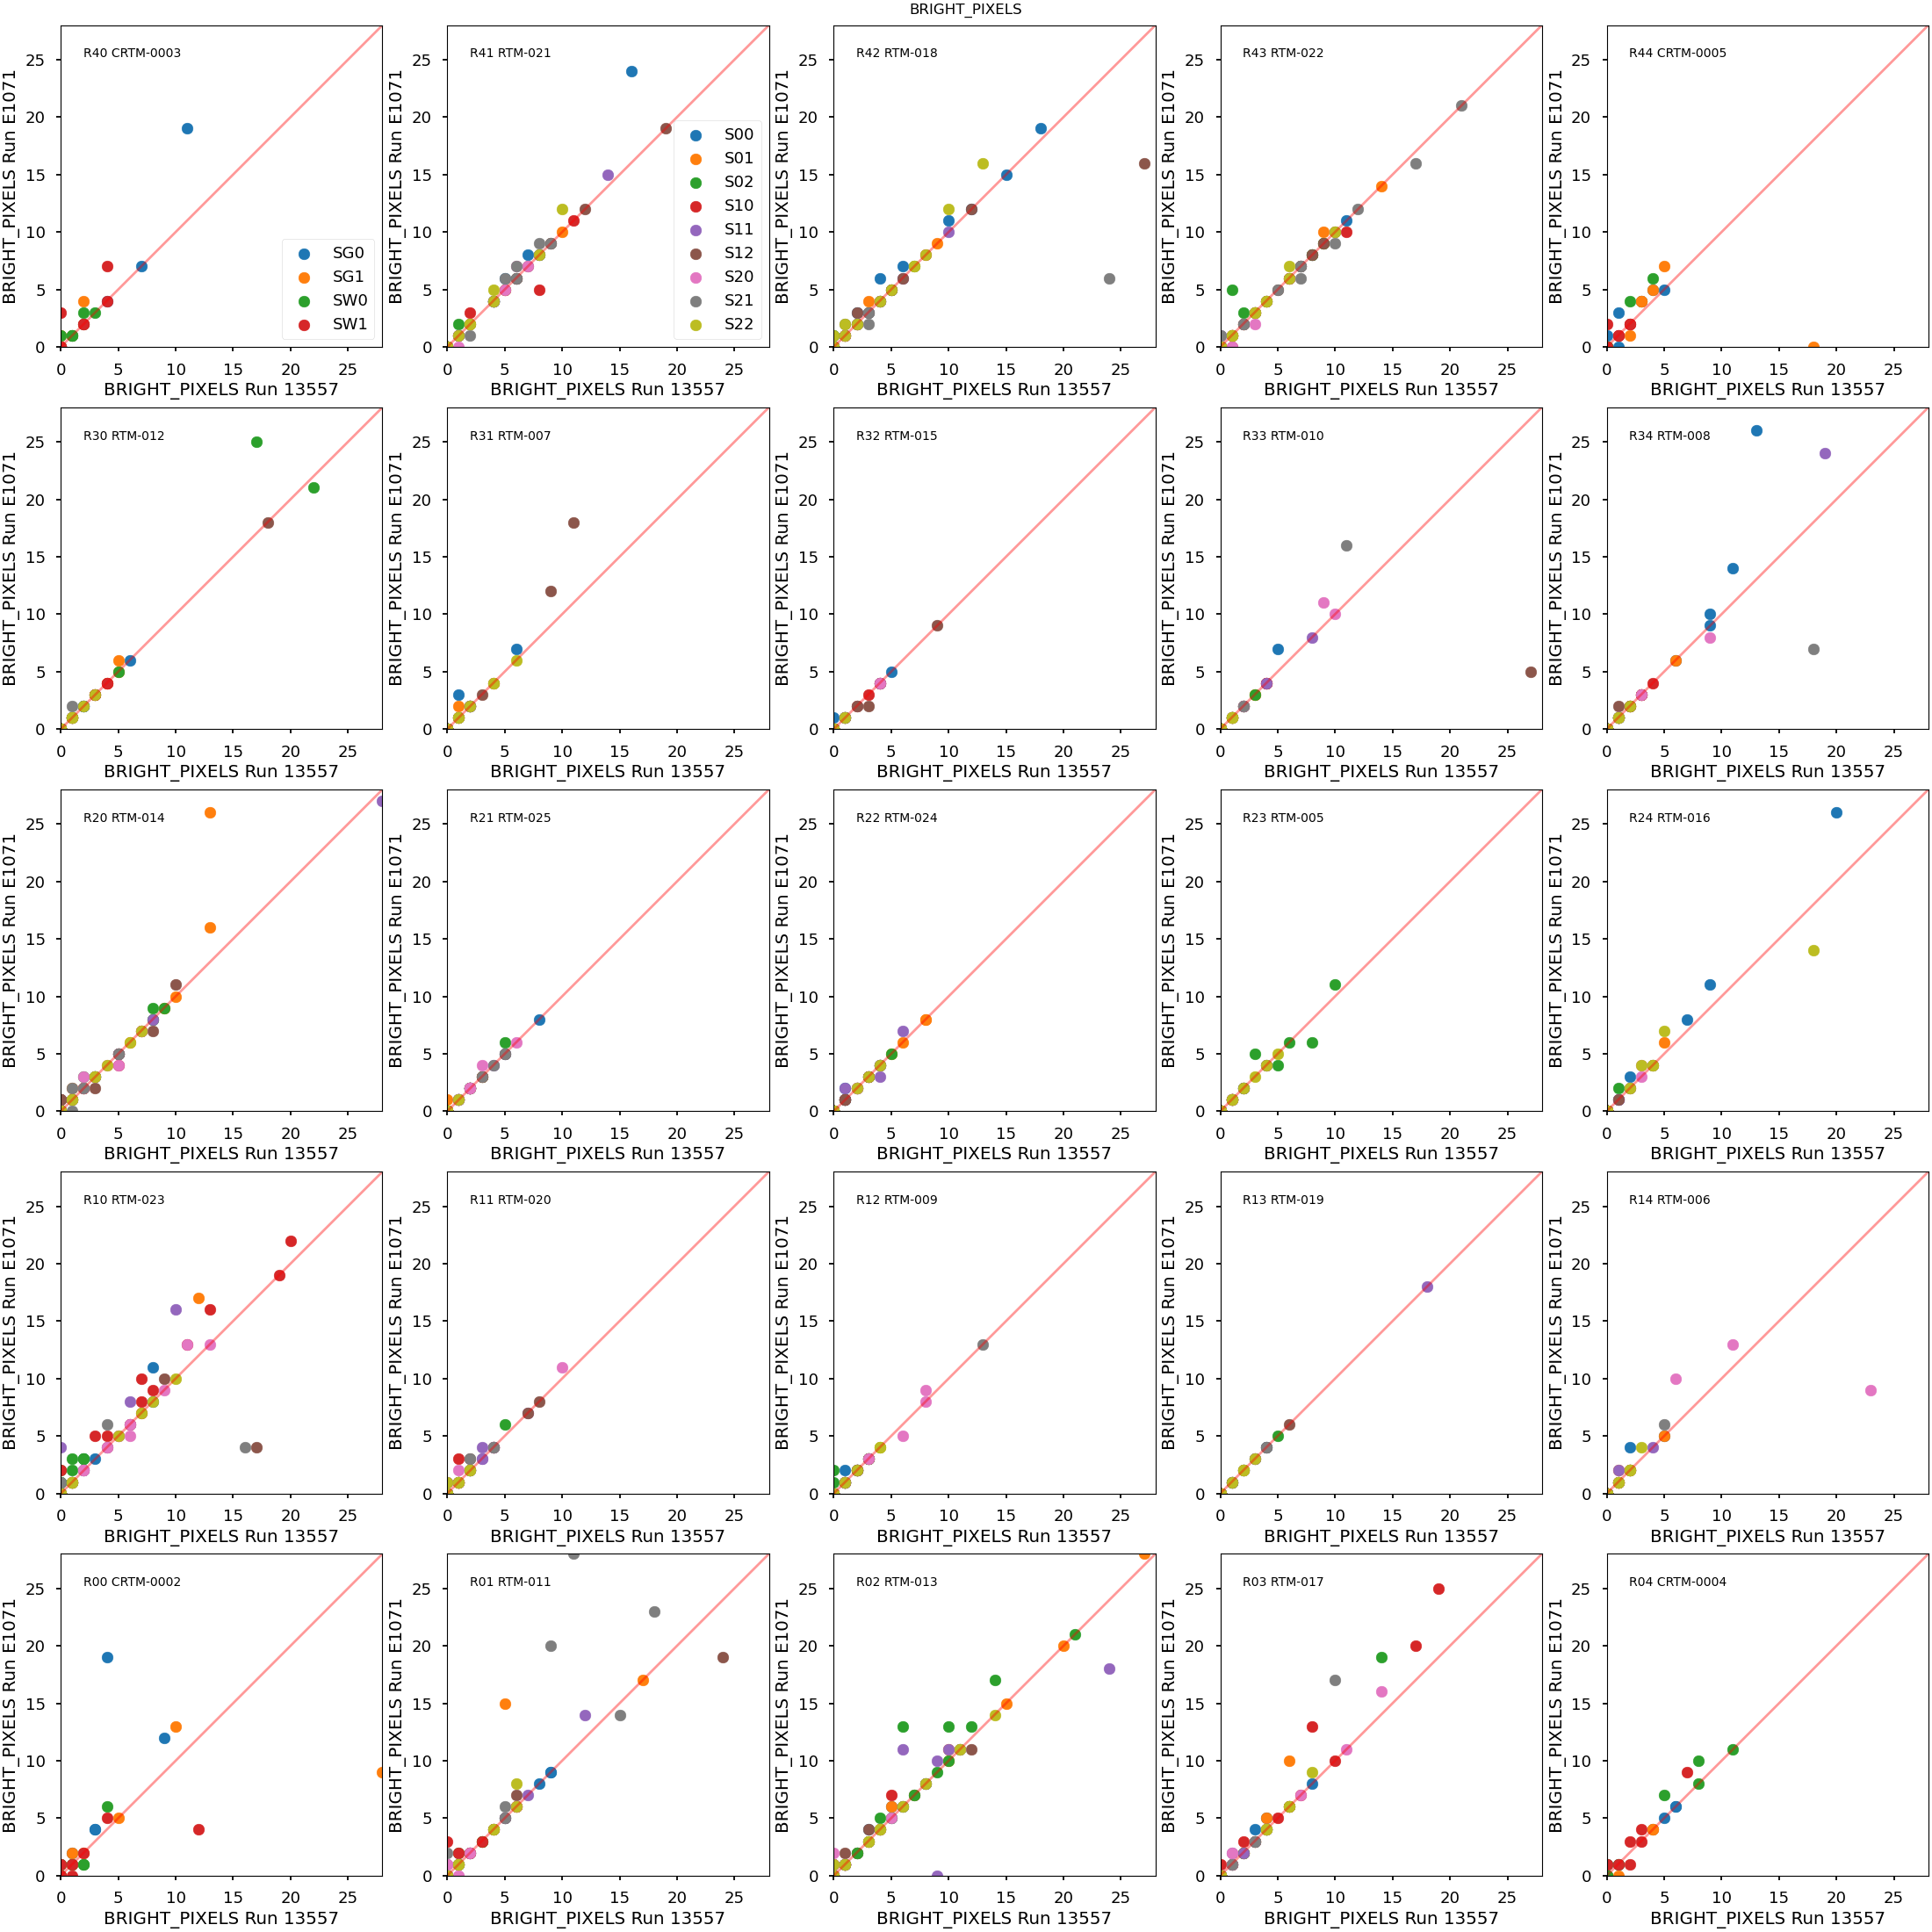
\includegraphics[width=0.7\textwidth]{sections/figures/baselineCharacterization/13557_E1071_BRIGHT_PIXELS.png}
\caption{}
\label{fig:bright}
\end{centering}
\end{figure}

Evaluating the change in defect counts on each amplifier segment between Run 6 and Run 7, and aggregating the amplifiers by the detector manufacturer shows a small increase of bright defects in Run 7 (Fig.~\ref{fig:dark-dist}). For ITL sensors, we find that 12\% of the amplifiers have more bright pixels than in Run 6. For e2v sensors, we find 4\% of the amplifiers that have more bright pixels. Despite this, the number of bright defects between runs does not increase for most sensors.

\begin{figure}[H]
\begin{centering}
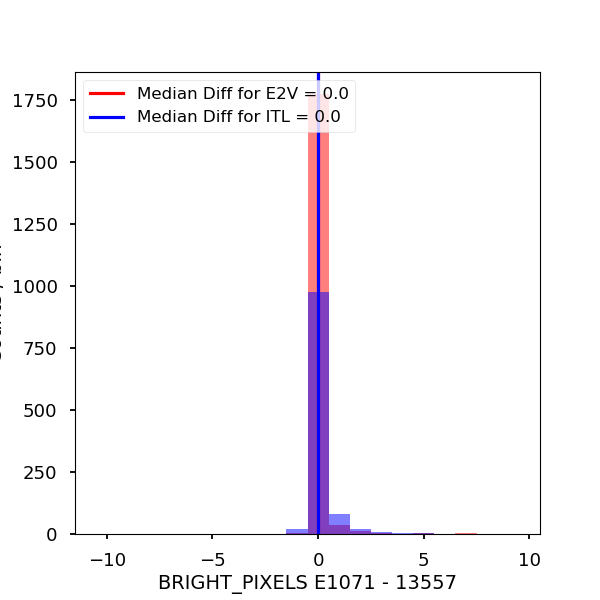
\includegraphics[width=0.7\textwidth]{sections/figures/baselineCharacterization/BRIGHT_PIXELS_13557_E1071_diff.png}
\caption{Distributions of differences in bright pixel count per amplifier between Run 7 (E1071) and Run 6 (13557), grouped by CCD type.}
\label{fig:dark-dist}
\end{centering}
\end{figure}

\subsection{Flat pair metrics}\label{flat-pair-metrics}

\begin{figure}[H]
\begin{centering}
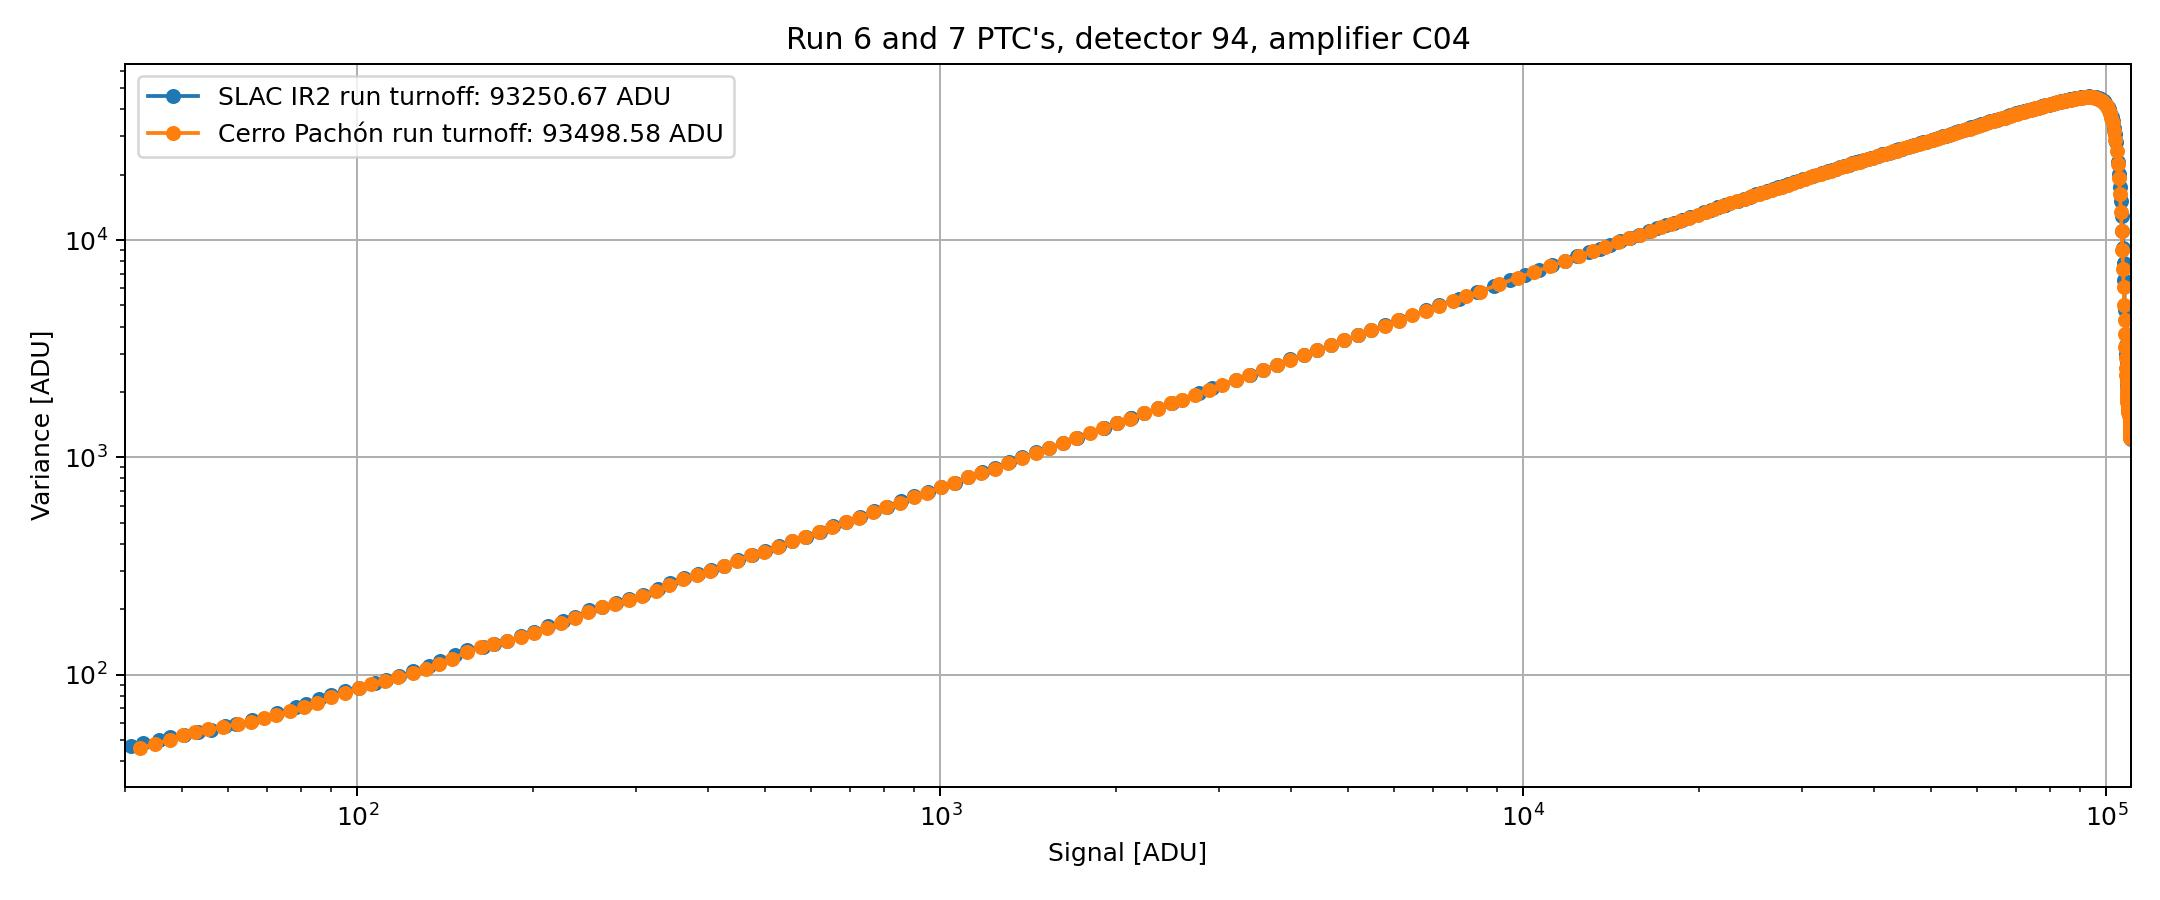
\includegraphics[width=0.95\textwidth]{sections/figures/baselineCharacterization/run7PTCsToDate.jpg}
\end{centering}
\end{figure}

\subsubsection{Linearity and PTC turnoff}\label{linearity-and-ptc-turnoff}

Linearity turnoff and PTC turnoff are two closely related metrics used
to characterize the upper limit of the usable signal range for accurate shape measurements and photometry. Linearity turnoff is the signal level above which the PTC curve deviates from
linearity and is measured for each amplifier segment of each CCD. We have defined the deviation threshold as 2\%.
PTC turnoff refers to the high-signal region of the PTC above which the PTC
variance decreases with increasing signal. This is due to saturation within the pixel wells of the CCDs. While slightly different, both metrics
provide important information about the upper limits of the dynamic
range in our sensors. Linearity turnoff is measured in units of e$^-$,
while PTC turnoff is measured in ADU.

\begin{figure}[H]
\begin{centering}
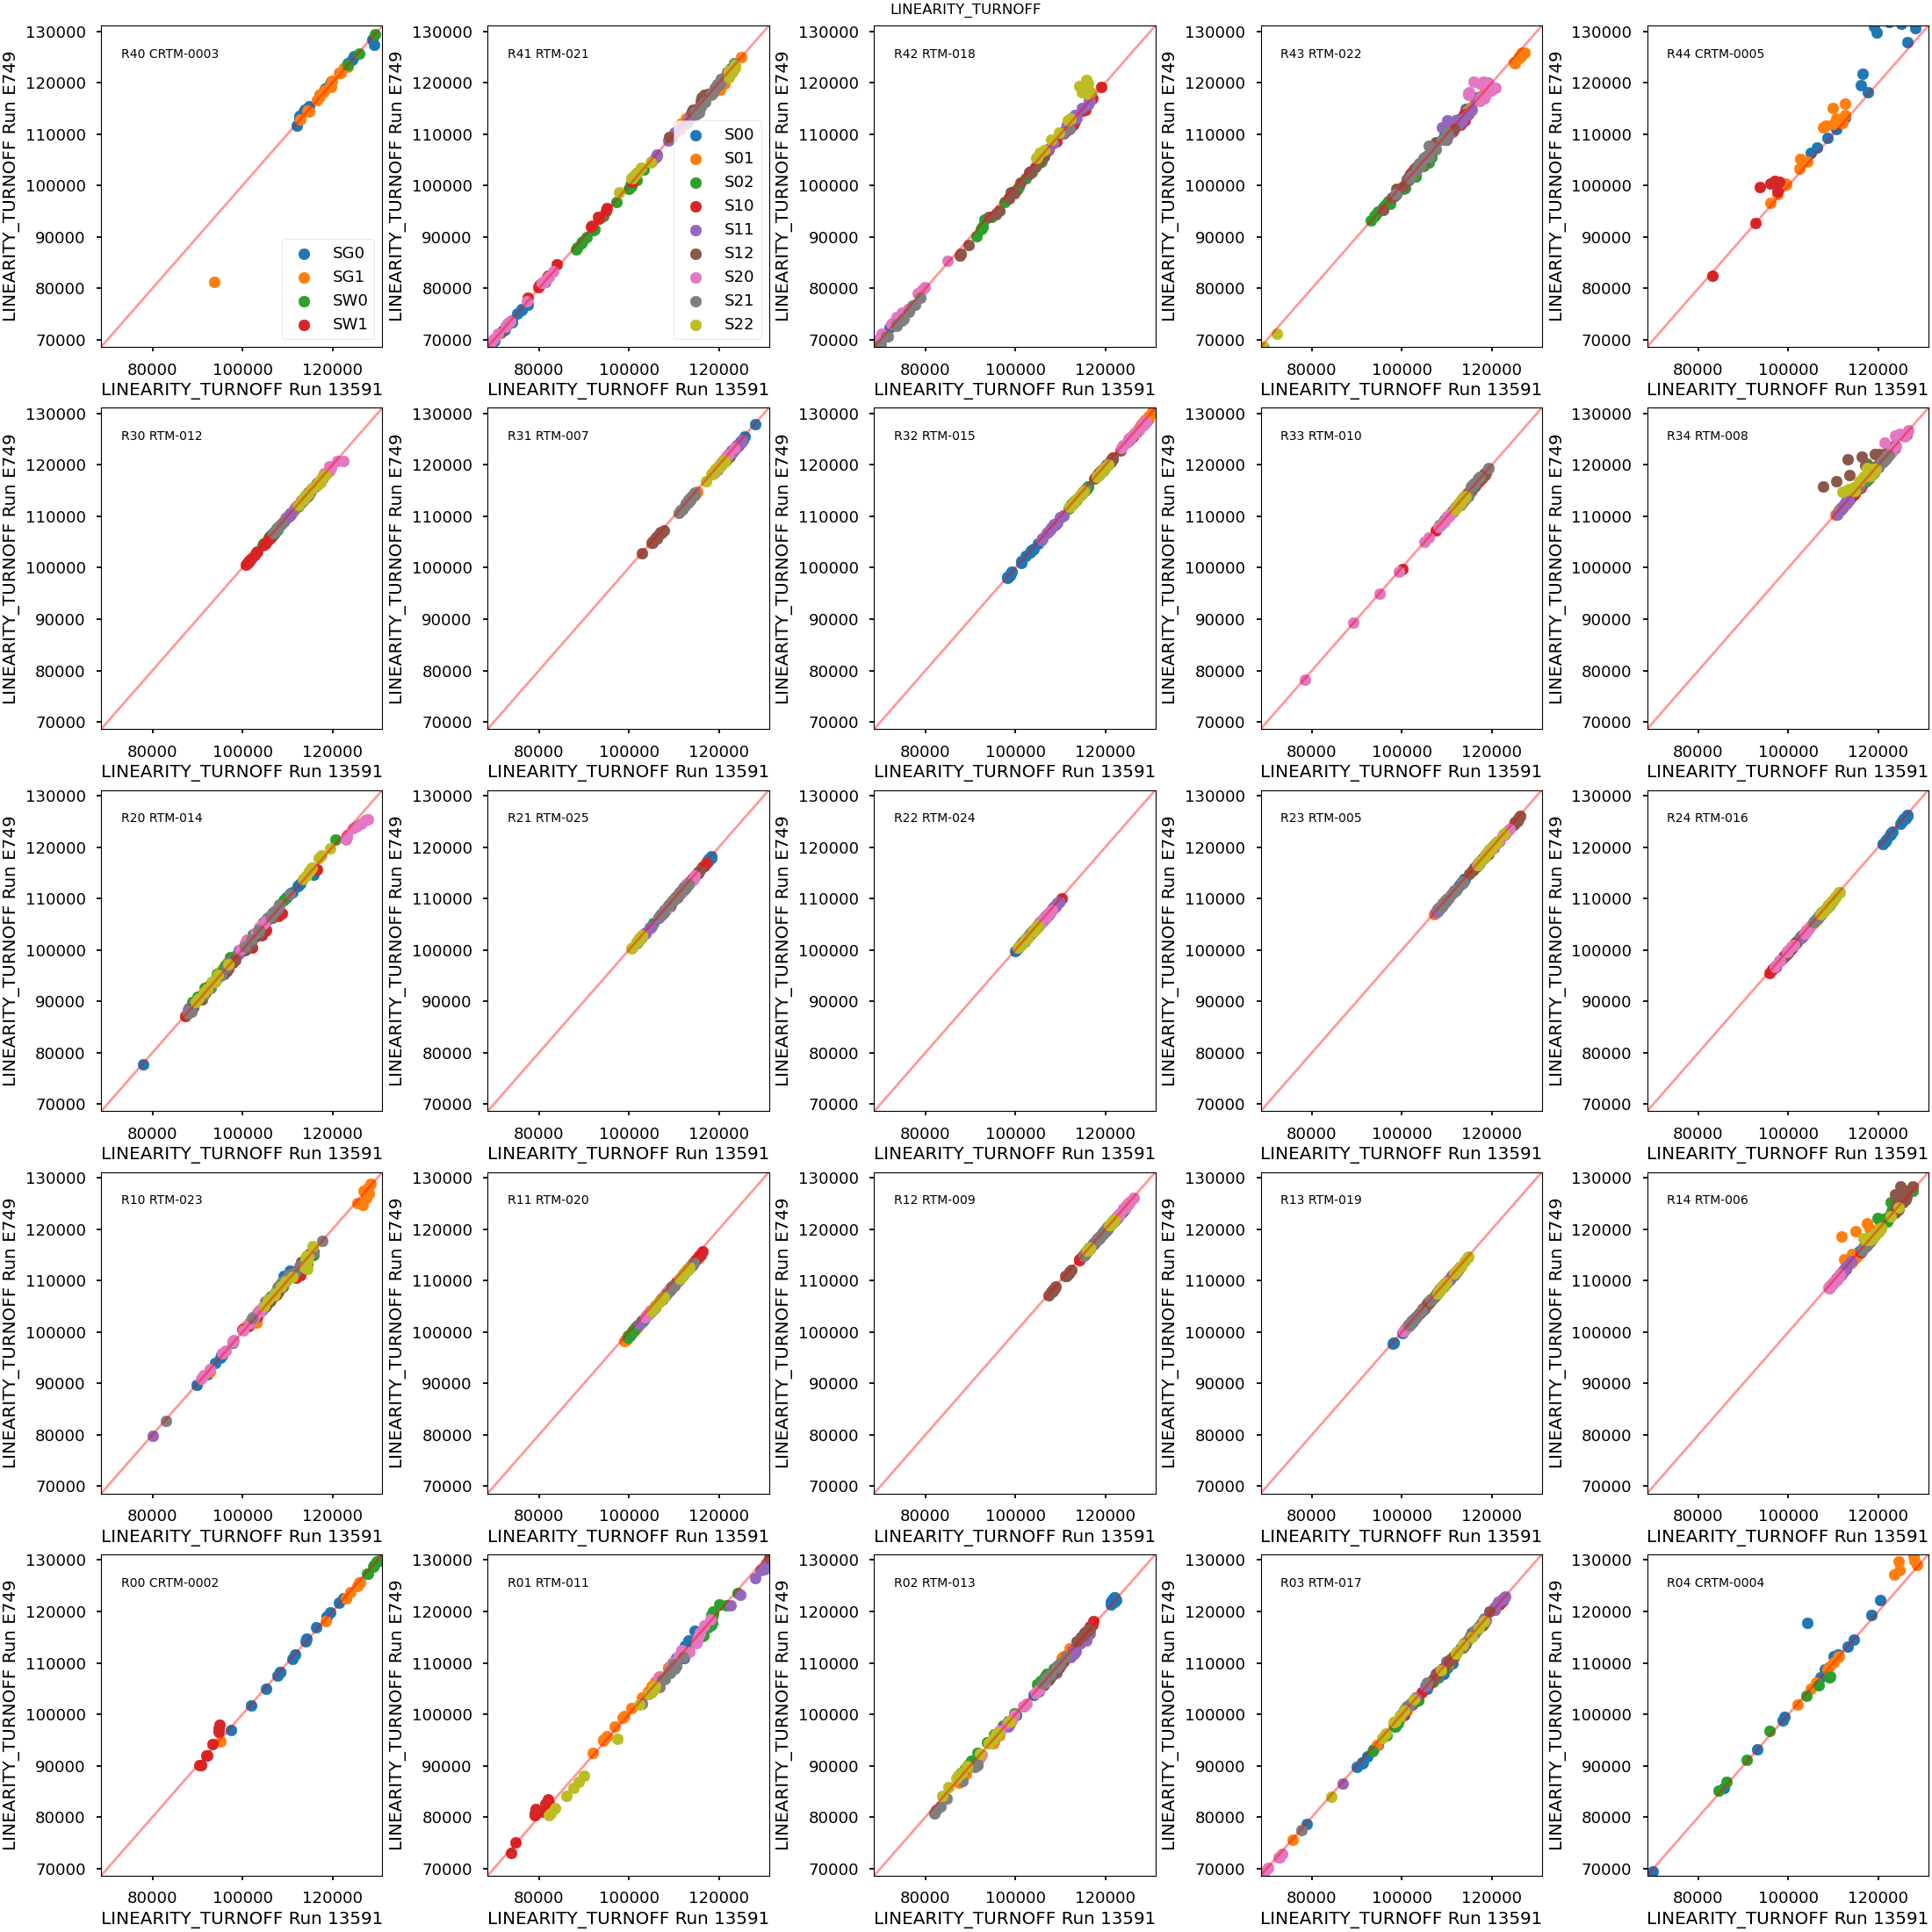
\includegraphics[width=0.7\textwidth]{sections/figures/baselineCharacterization/13591_E749_LINEARITY_TURNOFF.png}
\end{centering}
\end{figure}

In our linearity turnoff measurements, we find close agreement between
our Run 7 and Run 6 measurements for both ITL and e2v sensors.

\begin{figure}[H]
\begin{centering}
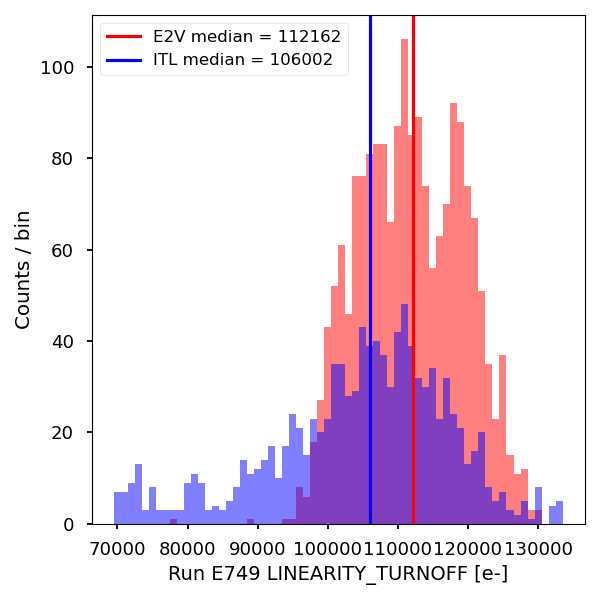
\includegraphics[width=0.7\textwidth]{sections/figures/baselineCharacterization/LINEARITY_TURNOFF_E749_sensorType.png}
\end{centering}
\end{figure}

Run 7 PTC turnoff measurements agree closely between run 6 and run 7, differing by \leq 200 e- for both ITL and E2V sensors. Notably, they are lower on average for both detector types.

\begin{figure}[H]
\begin{centering}
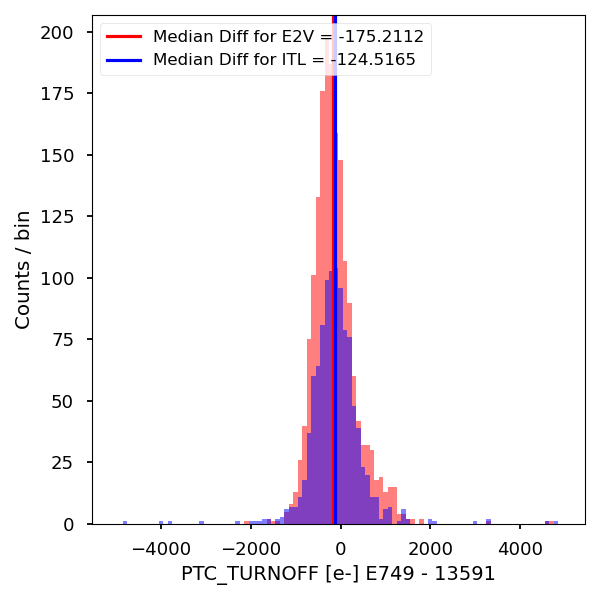
\includegraphics[width=0.7\textwidth]{sections/figures/baselineCharacterization/PTC_TURNOFF_13591_E749_diff.png}
\end{centering}
\end{figure}

\subsubsection{PTC Gain}\label{ptc-gain}

PTC gain is the conversion factor between digital output signal and the the number of electrons generated in the pixels of the CCD. It is one of the key parameters derived from the Photon Transfer
Curve, as it is the slope above the flux range at which the variance is dominated by shot
noise, and below the PTC turnoff. Gain is expressed in e$^-$/ADU, and scales the digitized analog signals from the ASPICs to units of e$^{-1}$.

\begin{figure}[H]
\begin{centering}
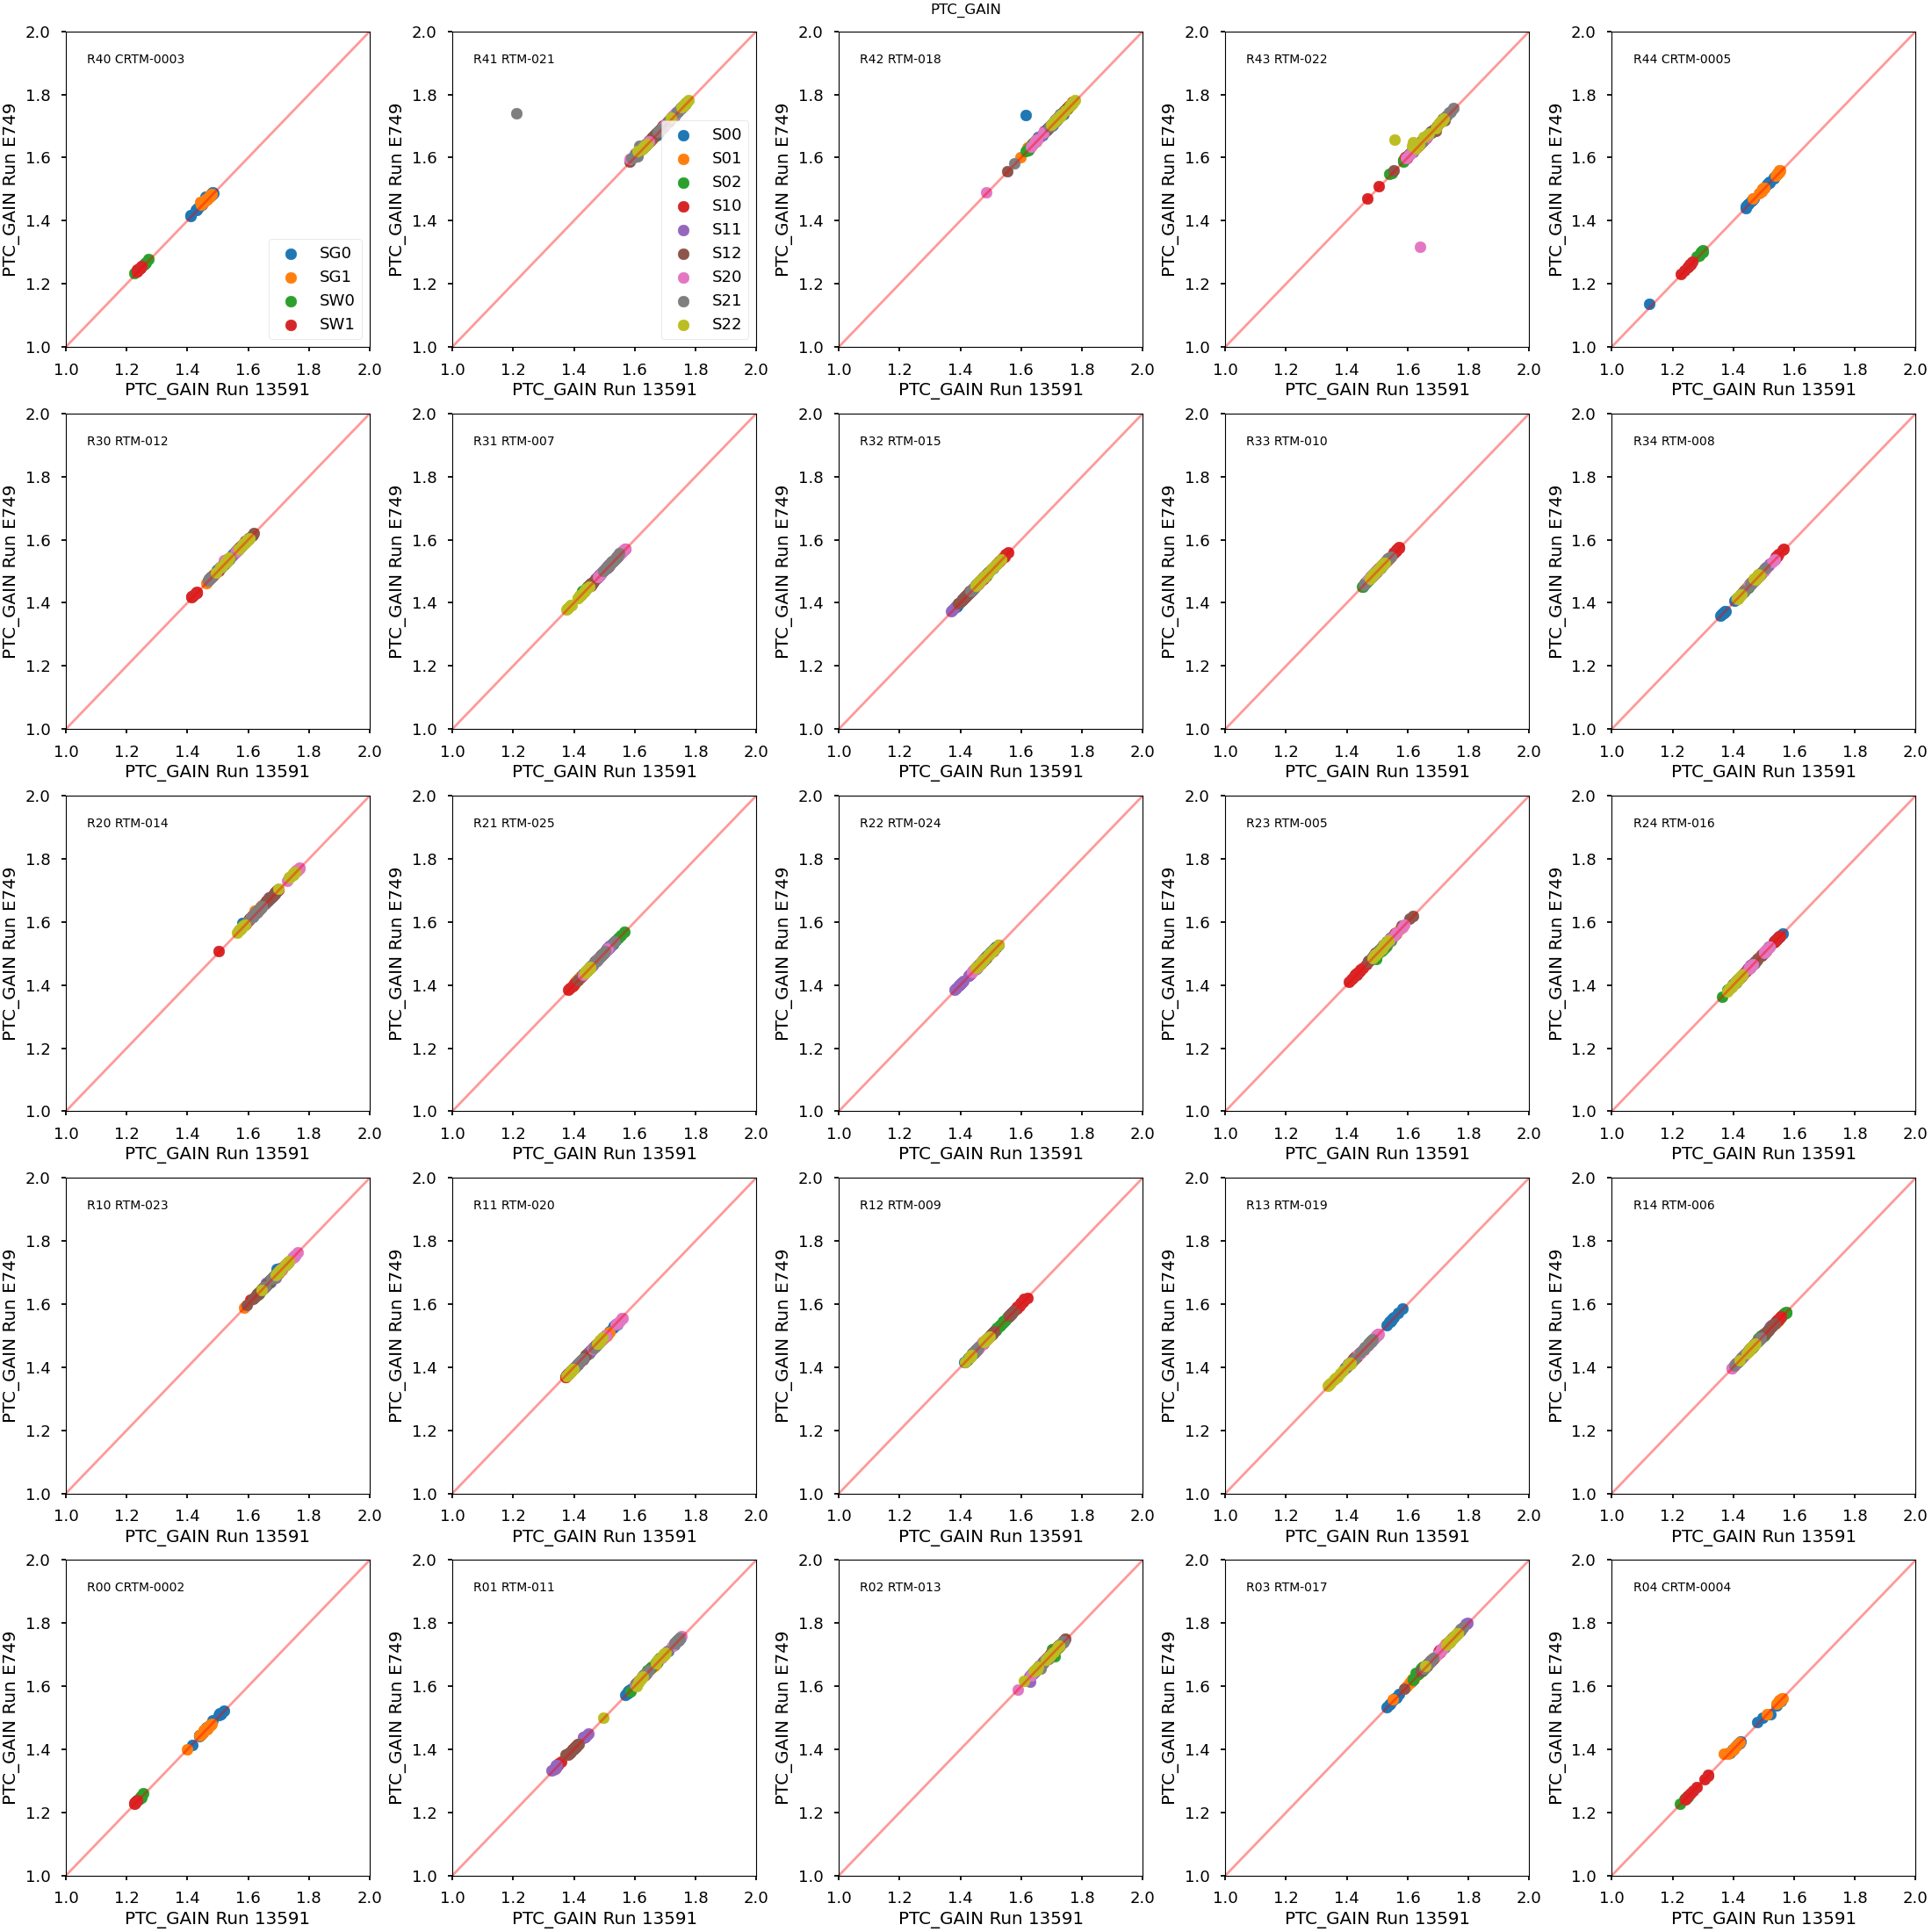
\includegraphics[width=0.7\textwidth]{sections/figures/baselineCharacterization/13591_E749_PTC_GAIN.png}
\end{centering}
\end{figure}

PTC gain measurements agree extremely closely across all sensors in the
focal plane.

\subsubsection{\texorpdfstring{Brighter fatter a{00}
coefficient}{Brighter fatter a00 coefficient}}\label{brighter-fatter-a00-coefficient}

This redistribution causes the charge to ``spill" into adjacent pixels, effectively broadening the point spread function (PSF). The brighter-fatter effect is the most dominant source of covariance in the PTC curve. The brighter-fatter effect in CCDs refers to the phenomenon where brighter pixels appear larger (or ``fatter" than dimmer ones). This occurs due to electrostatic interactions within the pixel wells of the CCDs, when a pixel accumulates a high charge from incoming photons and creates an electric field that slightly repels incoming charge carriers into neighboring pixels. The brighter fatter effect can be modeled as the most dominant source of pixel-pixel correlations. Following the PTC model from \hyperref[Astier]{{[}Astier{]}}, $a_{00}$ describes the change of a pixel area due to its own charge content, or the relative strength of the brighter-fatter effect. Since same-charge carriers repel each other, the pixel area decreases as charge accumulates inside the pixel well, which implies $a_{00}$ \textless{} 0. In eo\_pipe, an absolute value is taken of the $a_{00}$ parameter, so the tabulated quantities are positive.

\begin{figure}[H]
\begin{centering}
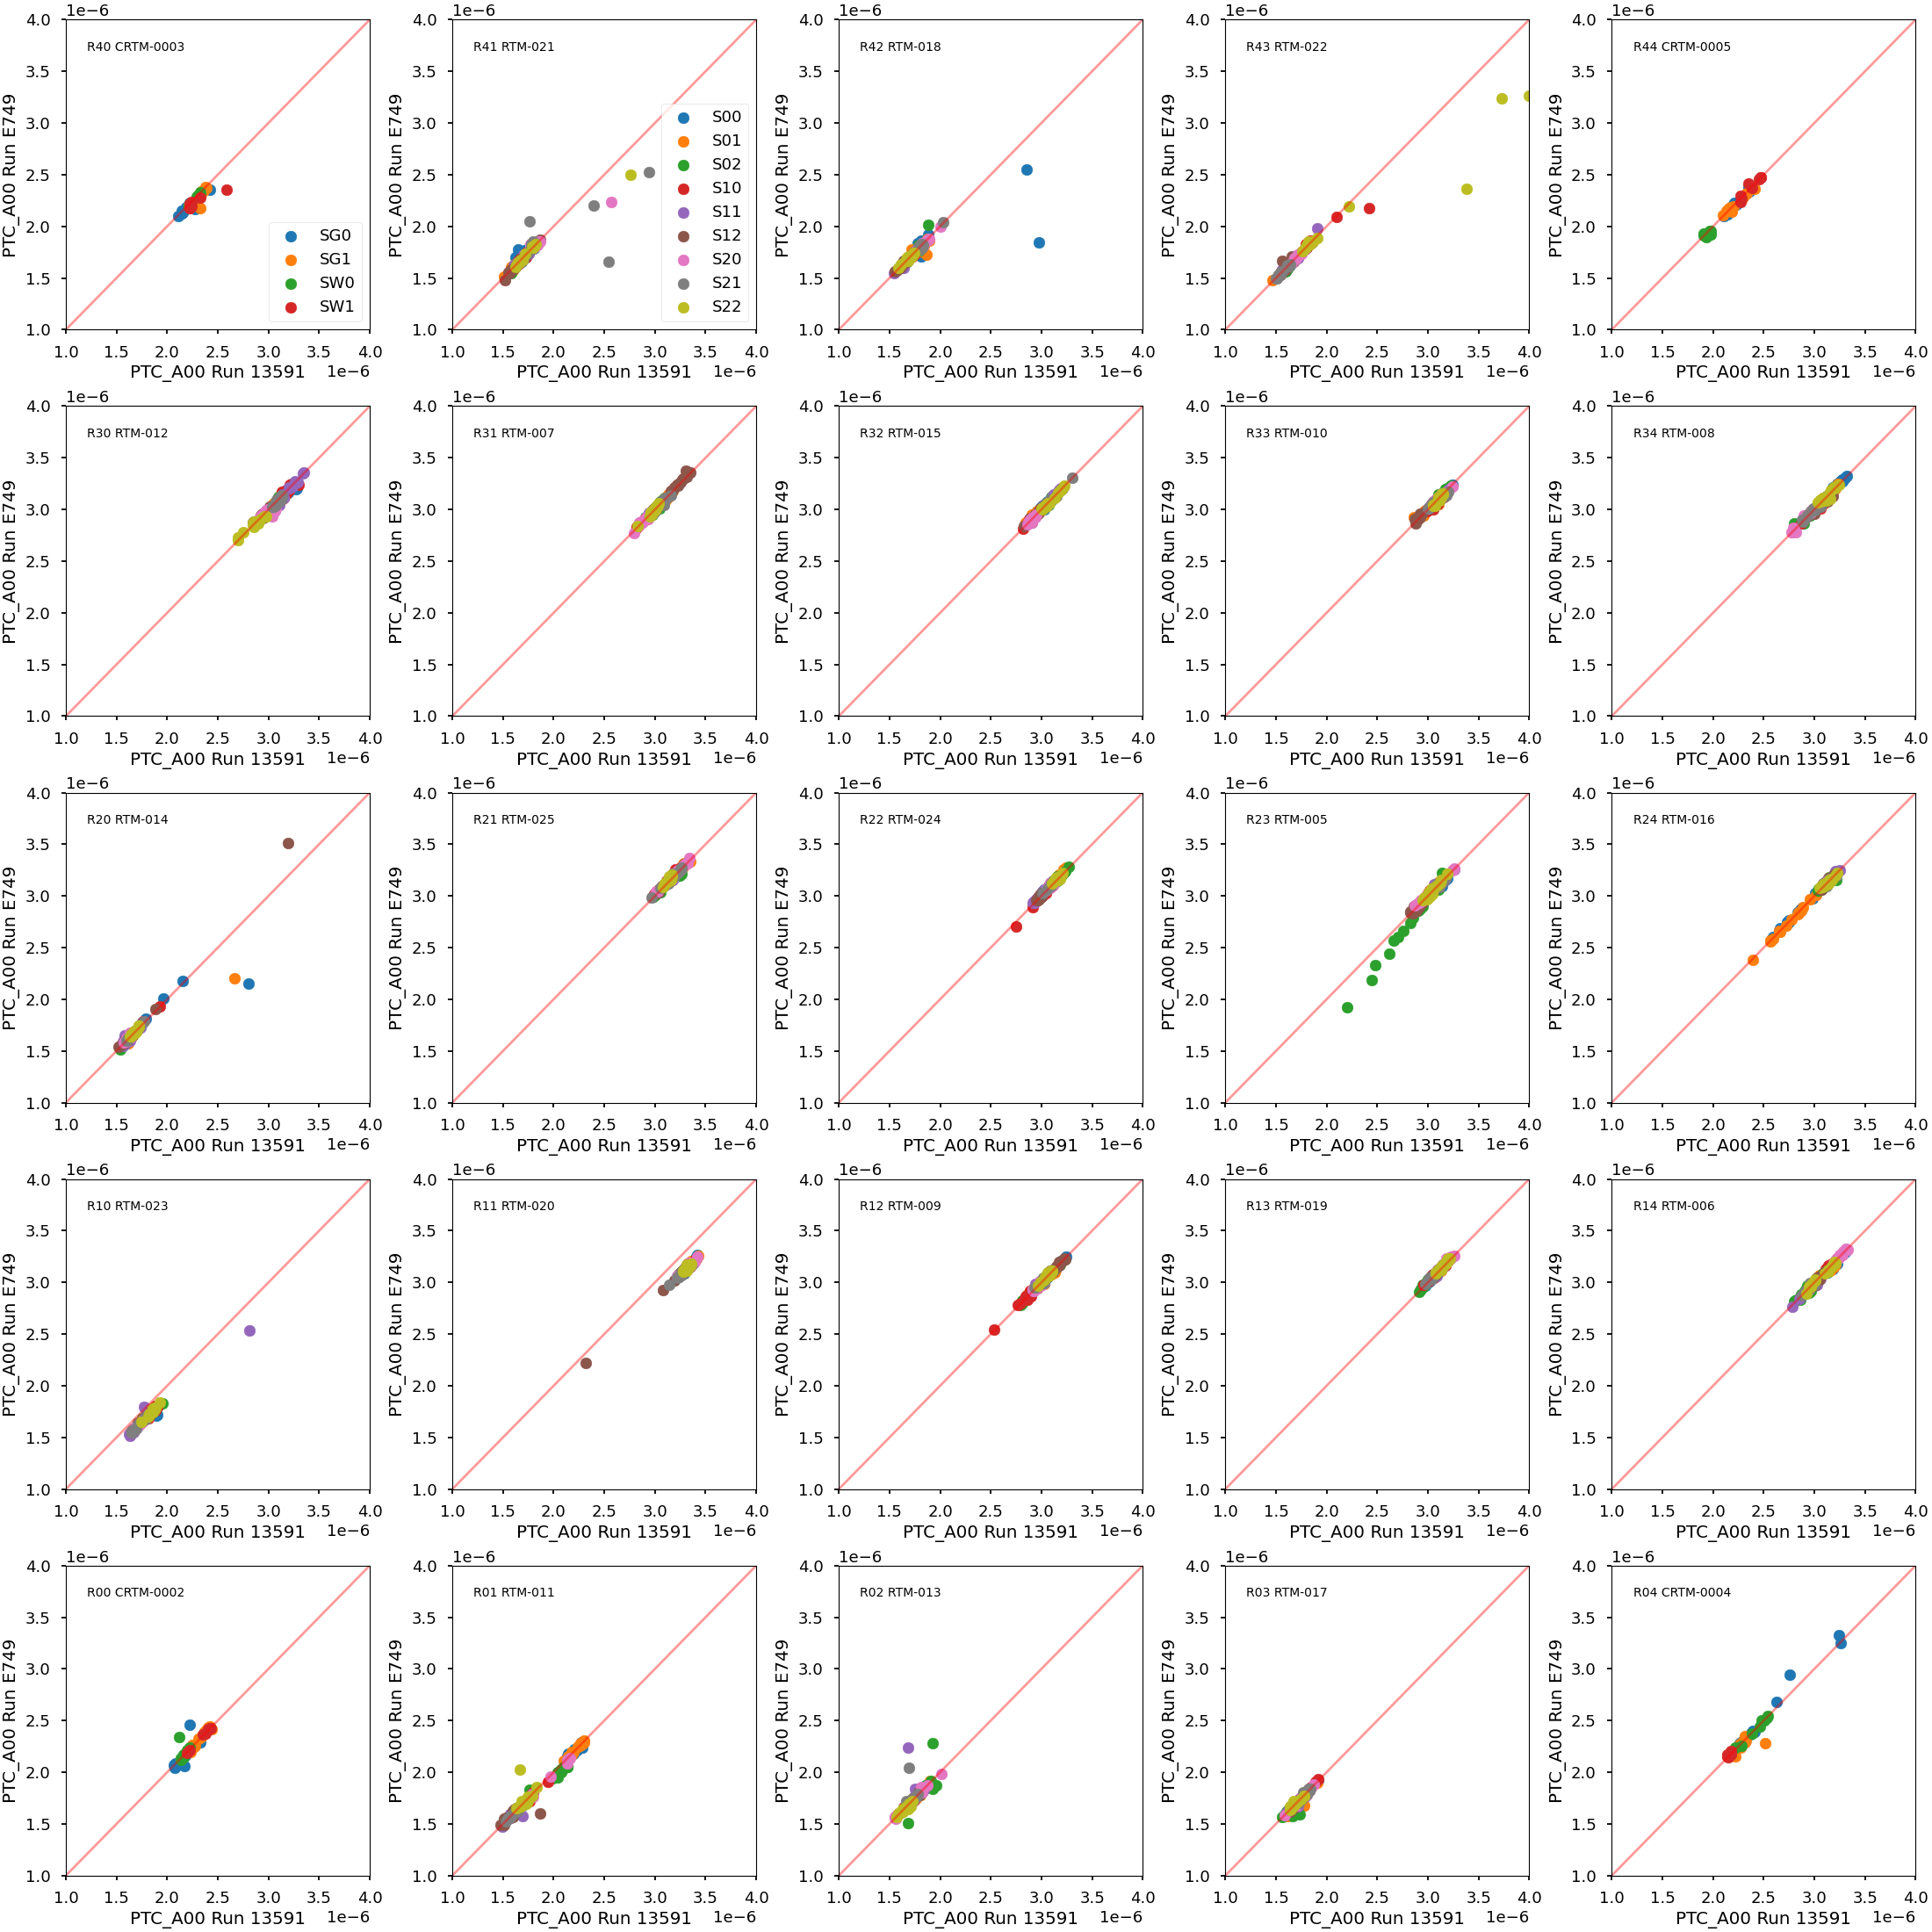
\includegraphics[width=0.7\textwidth]{sections/figures/baselineCharacterization/13591_E749_PTC_A00.png}
\end{centering}
\end{figure}

The strength of the brighter-fatter effect is generally comparable between Run 6 and Run 7. A few outliers exist across the
focal plane, of both CCD types.

\begin{figure}[H]
\begin{centering}
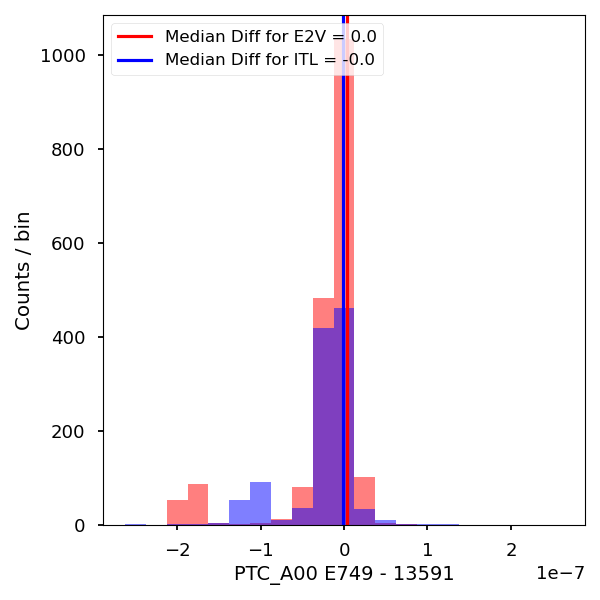
\includegraphics[width=0.7\textwidth]{sections/figures/baselineCharacterization/PTC_A00_13591_E749_diff.png}
\end{centering}
\end{figure}

However, the differences in the brighter-fatter $a_{00}$ coefficient between Run 6 and
Run 7 show that the magnitude of $a_{00}$ decreased for most
of the outliers, which implies an improvement in imaging for those pixels.

\subsubsection{Brighter-Fatter Correlation}\label{brighter-fatter-correlation}

The strength of the brighter fatter covariance correlation, and its subsequent error, provides a direct comparison of the PTC covariances across different runs.

\begin{figure}[H]
\begin{centering}
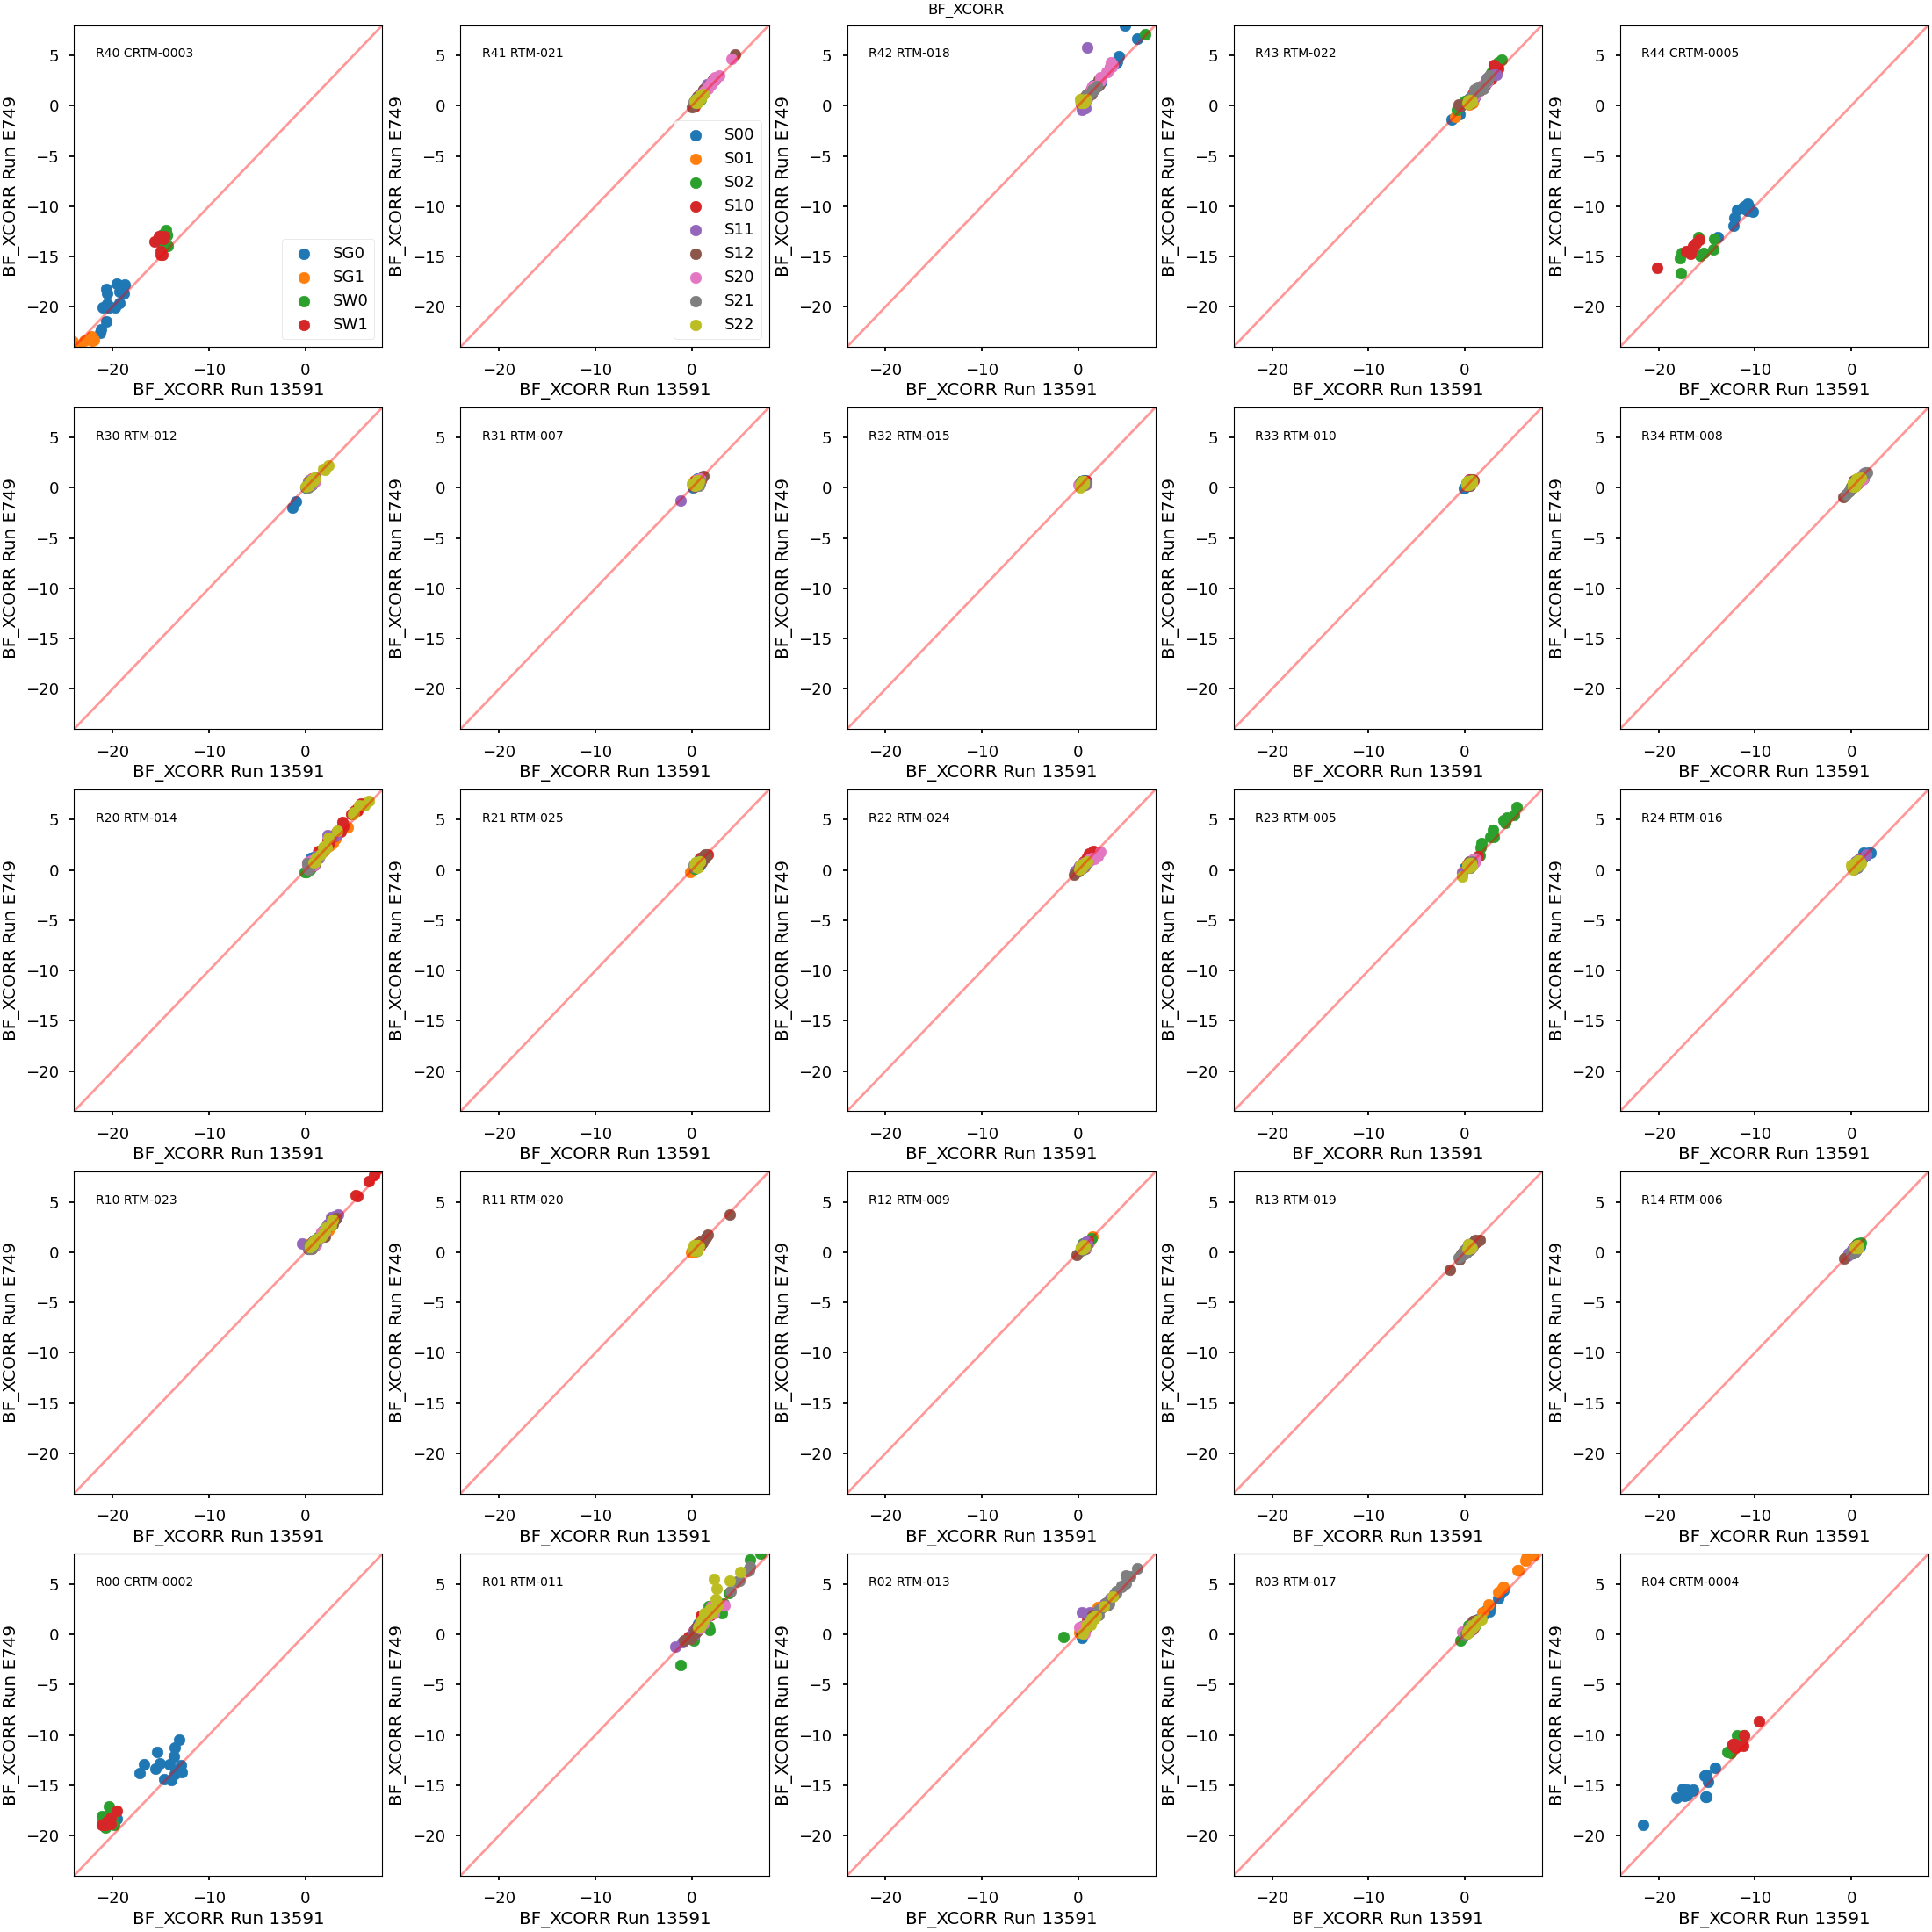
\includegraphics[width=0.7\textwidth]{sections/figures/baselineCharacterization/13591_E749_BF_XCORR.png}
\end{centering}
\end{figure}

\begin{figure}[H]
\begin{centering}
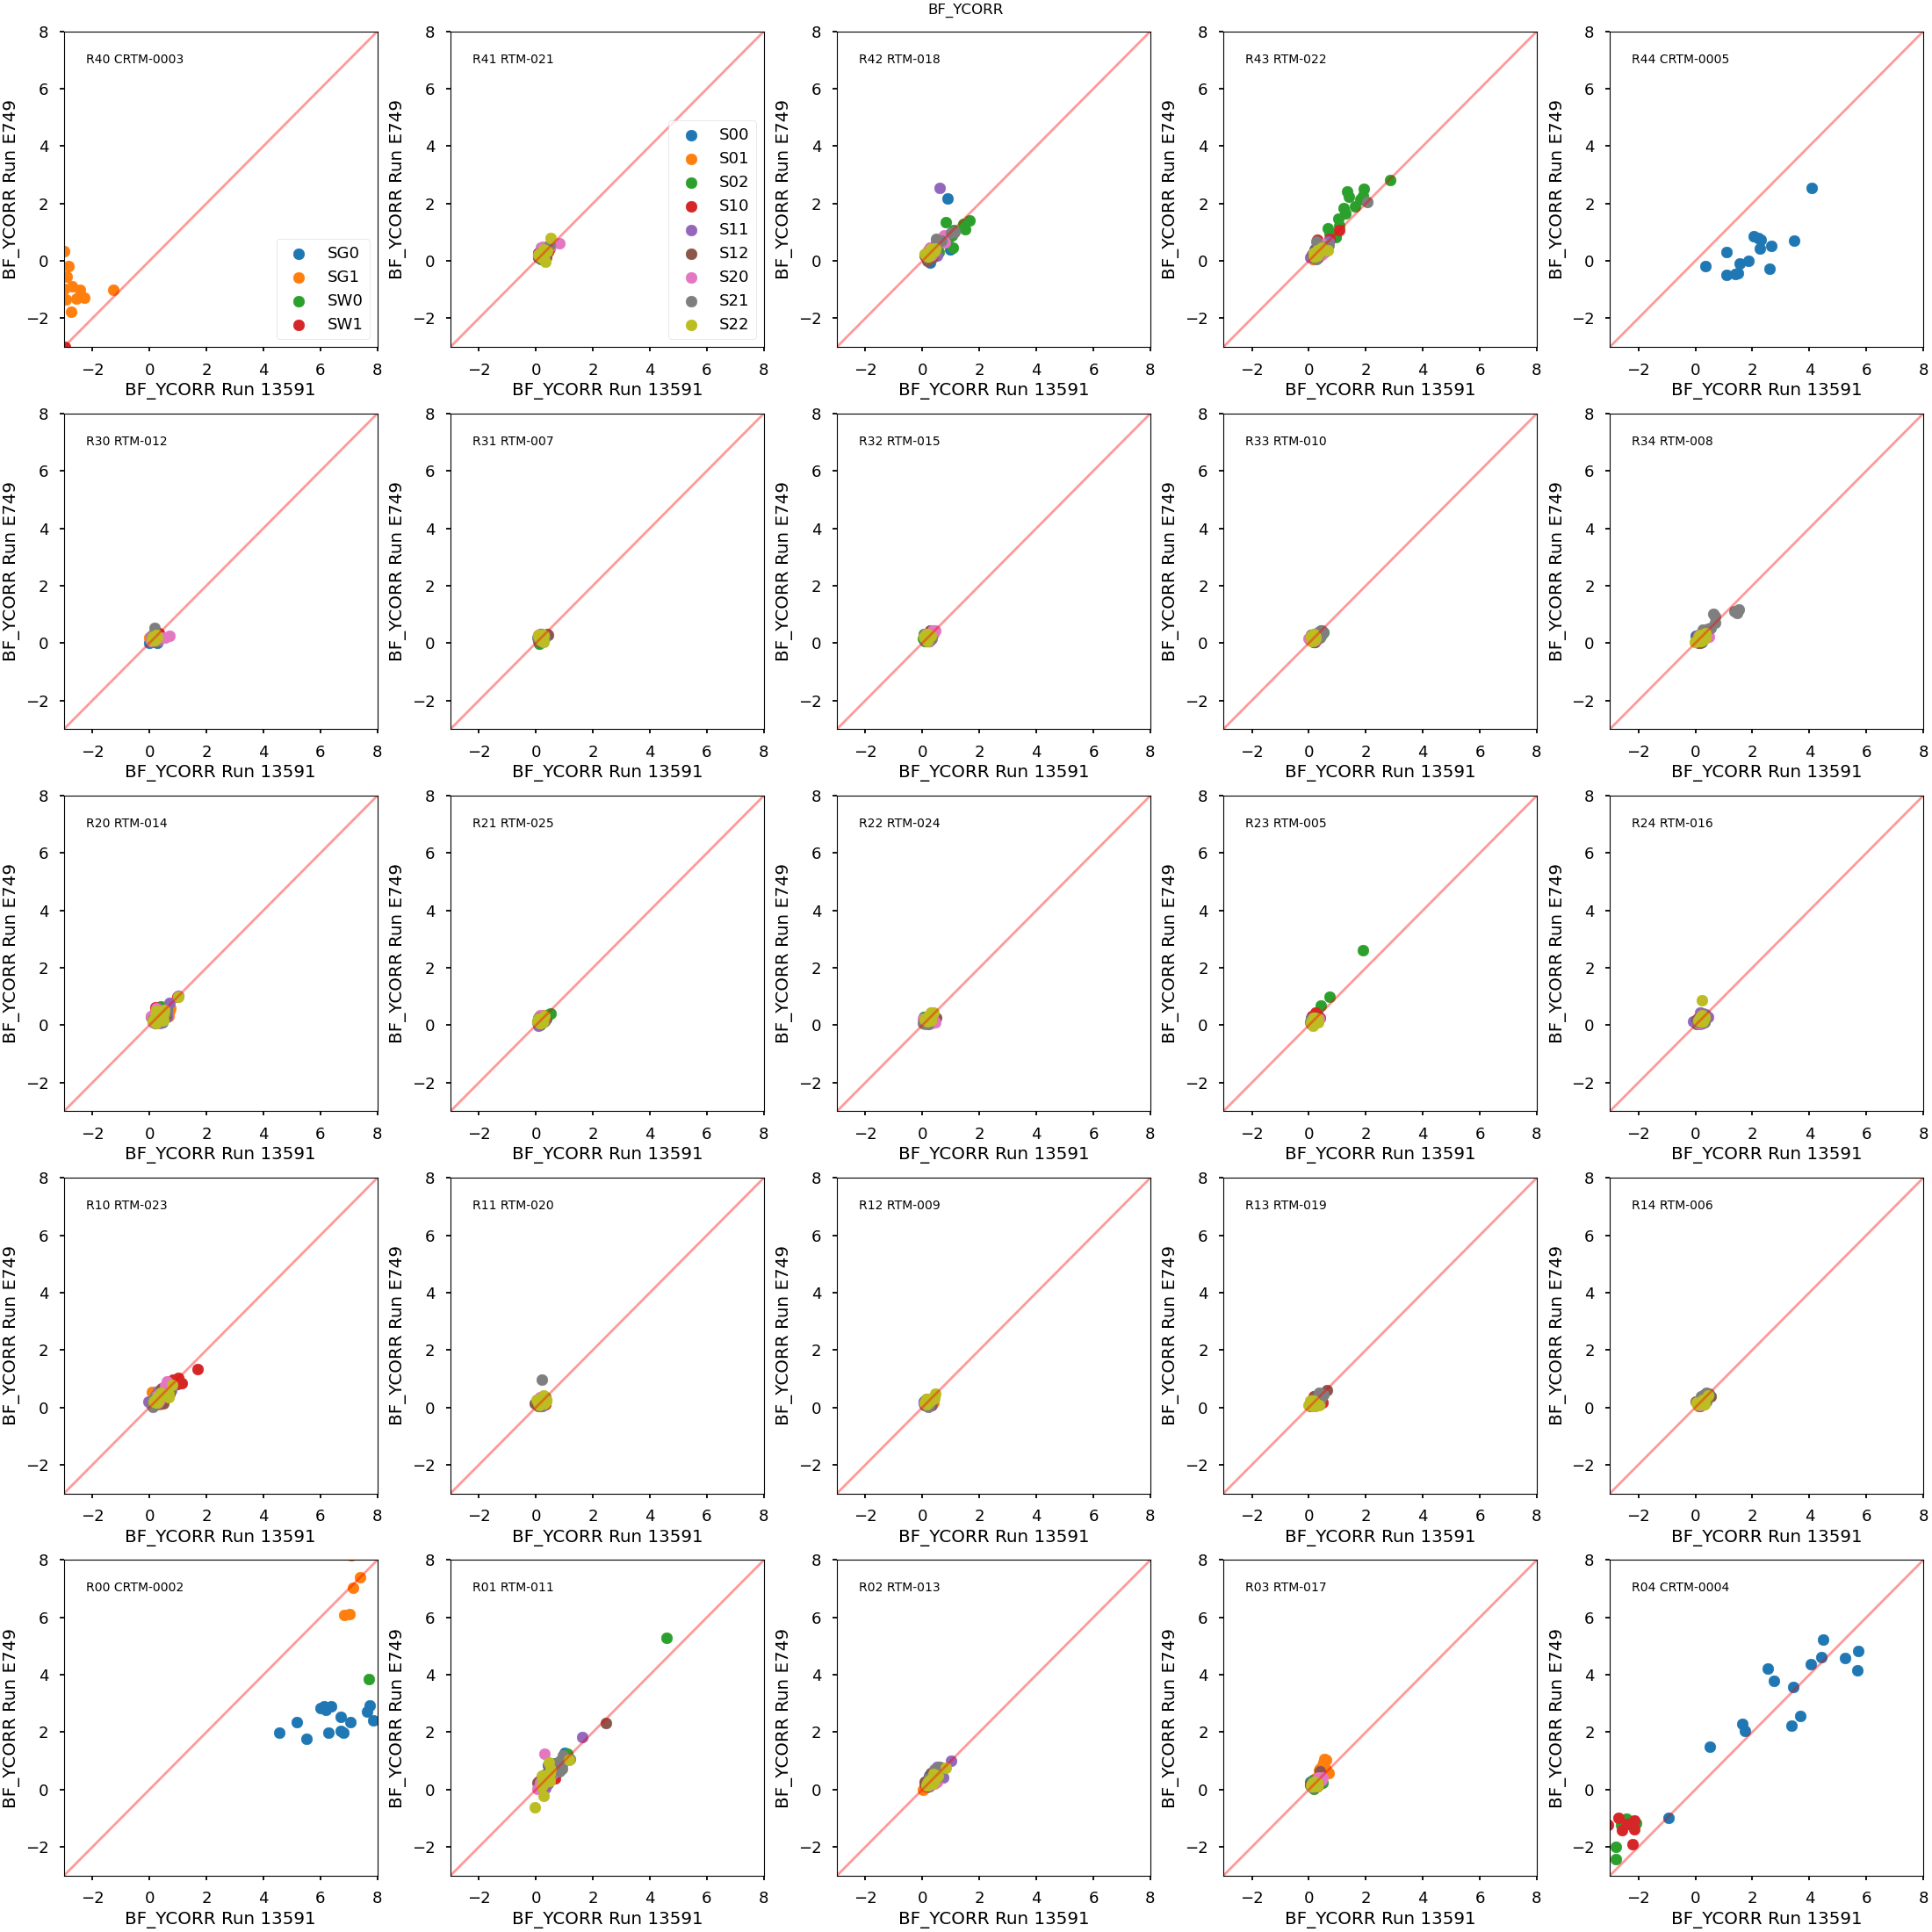
\includegraphics[width=0.7\textwidth]{sections/figures/baselineCharacterization/13591_E749_BF_YCORR.png}
\end{centering}
\end{figure}

The brighter-fatter correlation is comparable across different runs, regardless of detector type. The strongest deviation comes from a lower Run 7 x-correlation, with a difference of \textasciitilde0.07, which is negligible.

\begin{figure}[H]
\begin{centering}
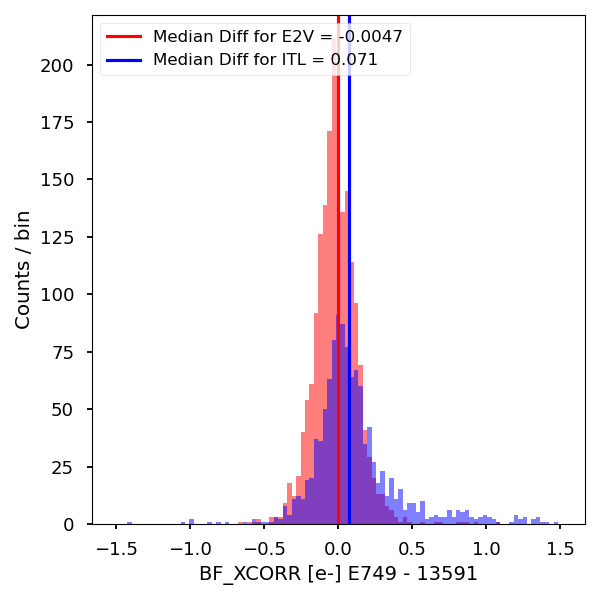
\includegraphics[width=0.7\textwidth]{sections/figures/baselineCharacterization/BF_XCORR_13591_E749_diff.png}
\end{centering}
\end{figure}

\begin{figure}[H]
\begin{centering}
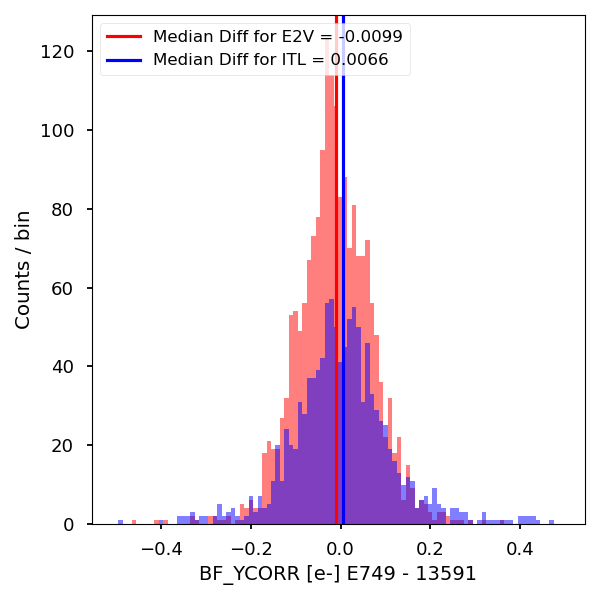
\includegraphics[width=0.7\textwidth]{sections/figures/baselineCharacterization/BF_YCORR_13591_E749_diff.png}
\end{centering}
\end{figure}

\subsubsection{Row-means variance}\label{row-means-var}

Row-means variance is a metric that measures the row to row variance in flat frames. By computing the ratio of the row variance (or measured variance) to the expected Poisson signal (or expected variance) at the flux level, we can measure if additional noise enters the PTC curve at any point.

\begin{figure}[H]
\begin{centering}
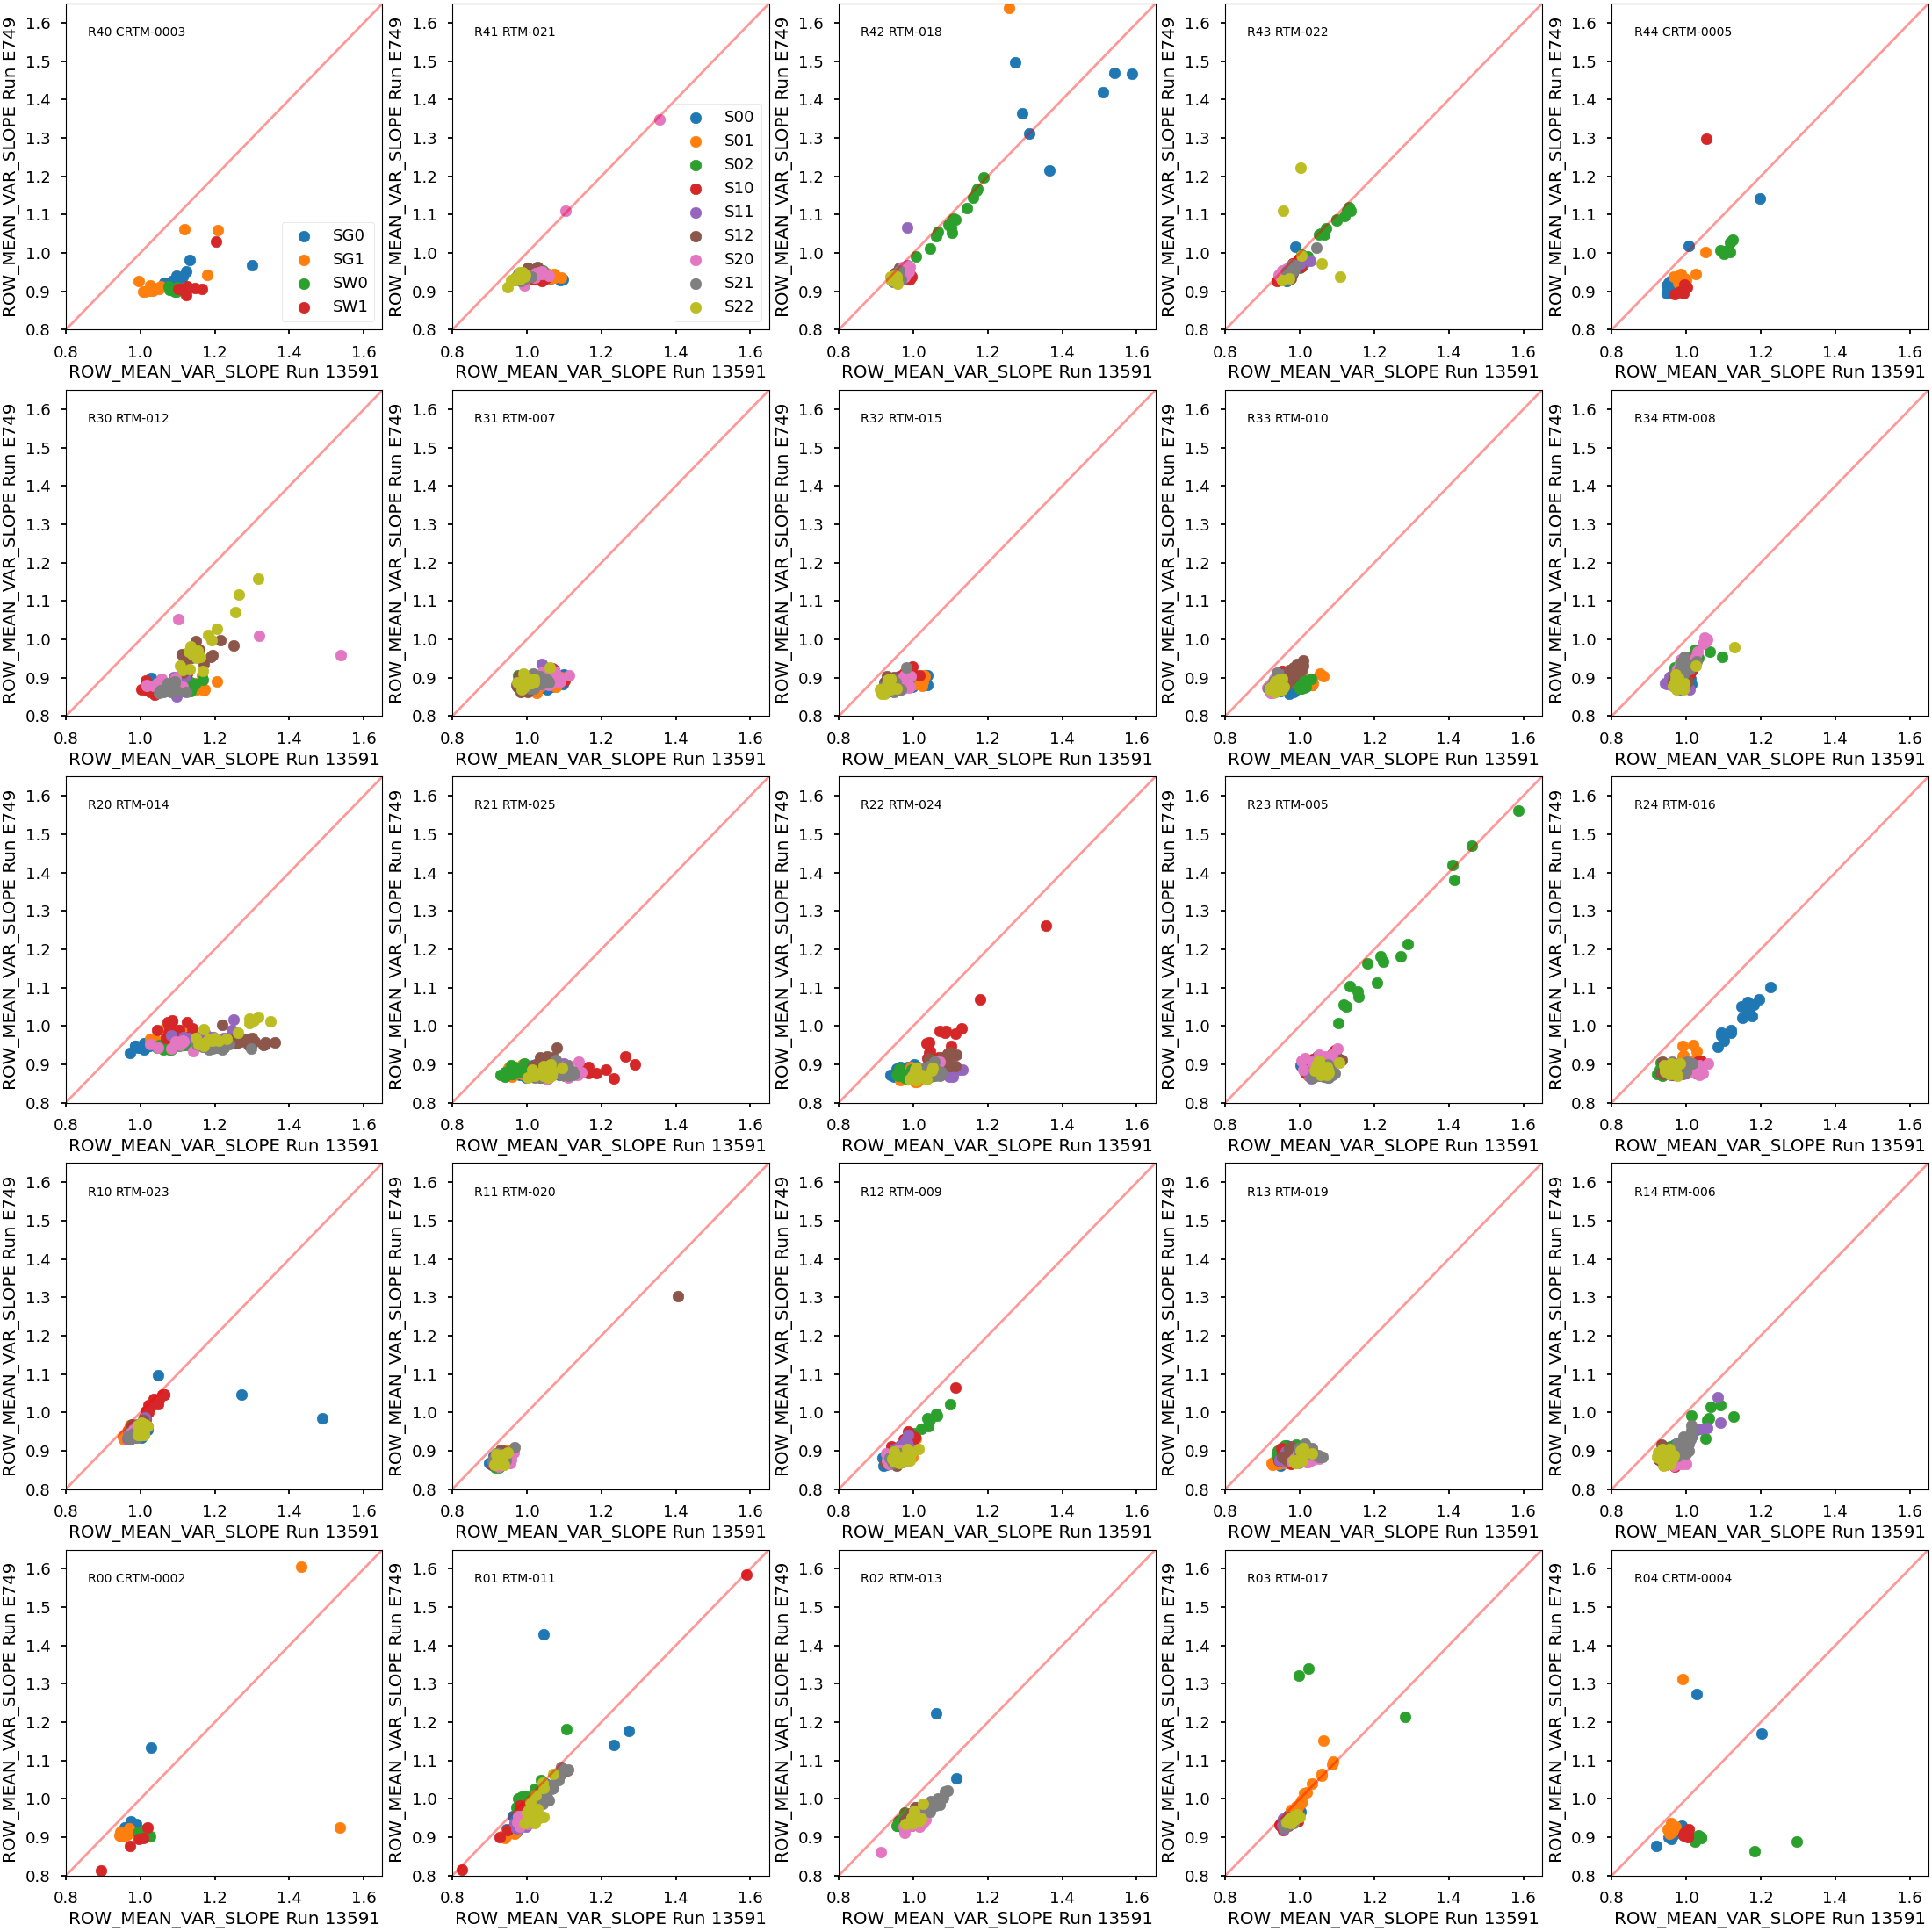
\includegraphics[width=0.7\textwidth]{sections/figures/baselineCharacterization/13591_E749_ROW_MEAN_VAR_SLOPE.png}
\end{centering}
\end{figure}

Differences in row-means variance between runs are evident, and are distinctly different for different detector types. The difference between runs is more significant for ITL sensors, \textasciitilde9\% smaller on average in Run 7. For E2V sensors, the effect is \textasciitilde3\% smaller in Run 7. This indicates that the non-shot noise contributions to sensor noise are smaller in run 7 compared to run 6, a positive result for the camera.

\begin{figure}[H]
\begin{centering}
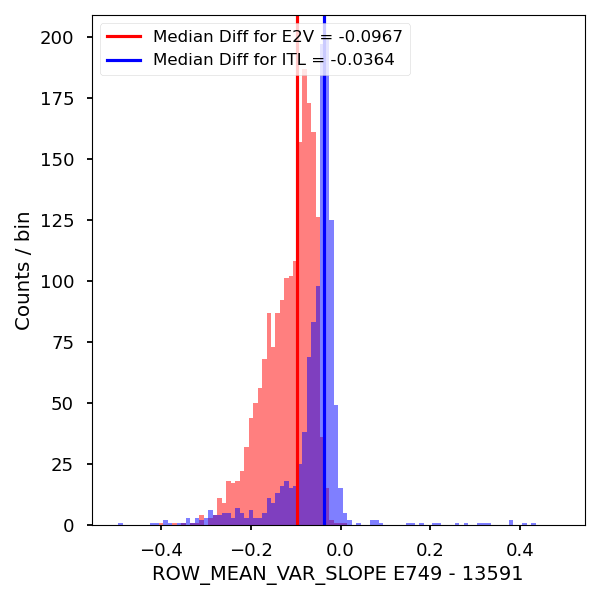
\includegraphics[width=0.7\textwidth]{sections/figures/baselineCharacterization/ROW_MEAN_VAR_SLOPE_13591_E749_diff.png}
\end{centering}
\end{figure}

\subsubsection{Divisadero Tearing}\label{divisadero-tearing}

Divisadero tearing is manifested as signal variations near amplifier boundaries, connected features that are often jagged. These variations are on the order of \textasciitilde1\% relative to the flat field signal. To quantify divisadero tearing in a given column, we measure the column signal, and compare it to the mean column signal from flat fields.

\begin{figure}[H]
\begin{centering}
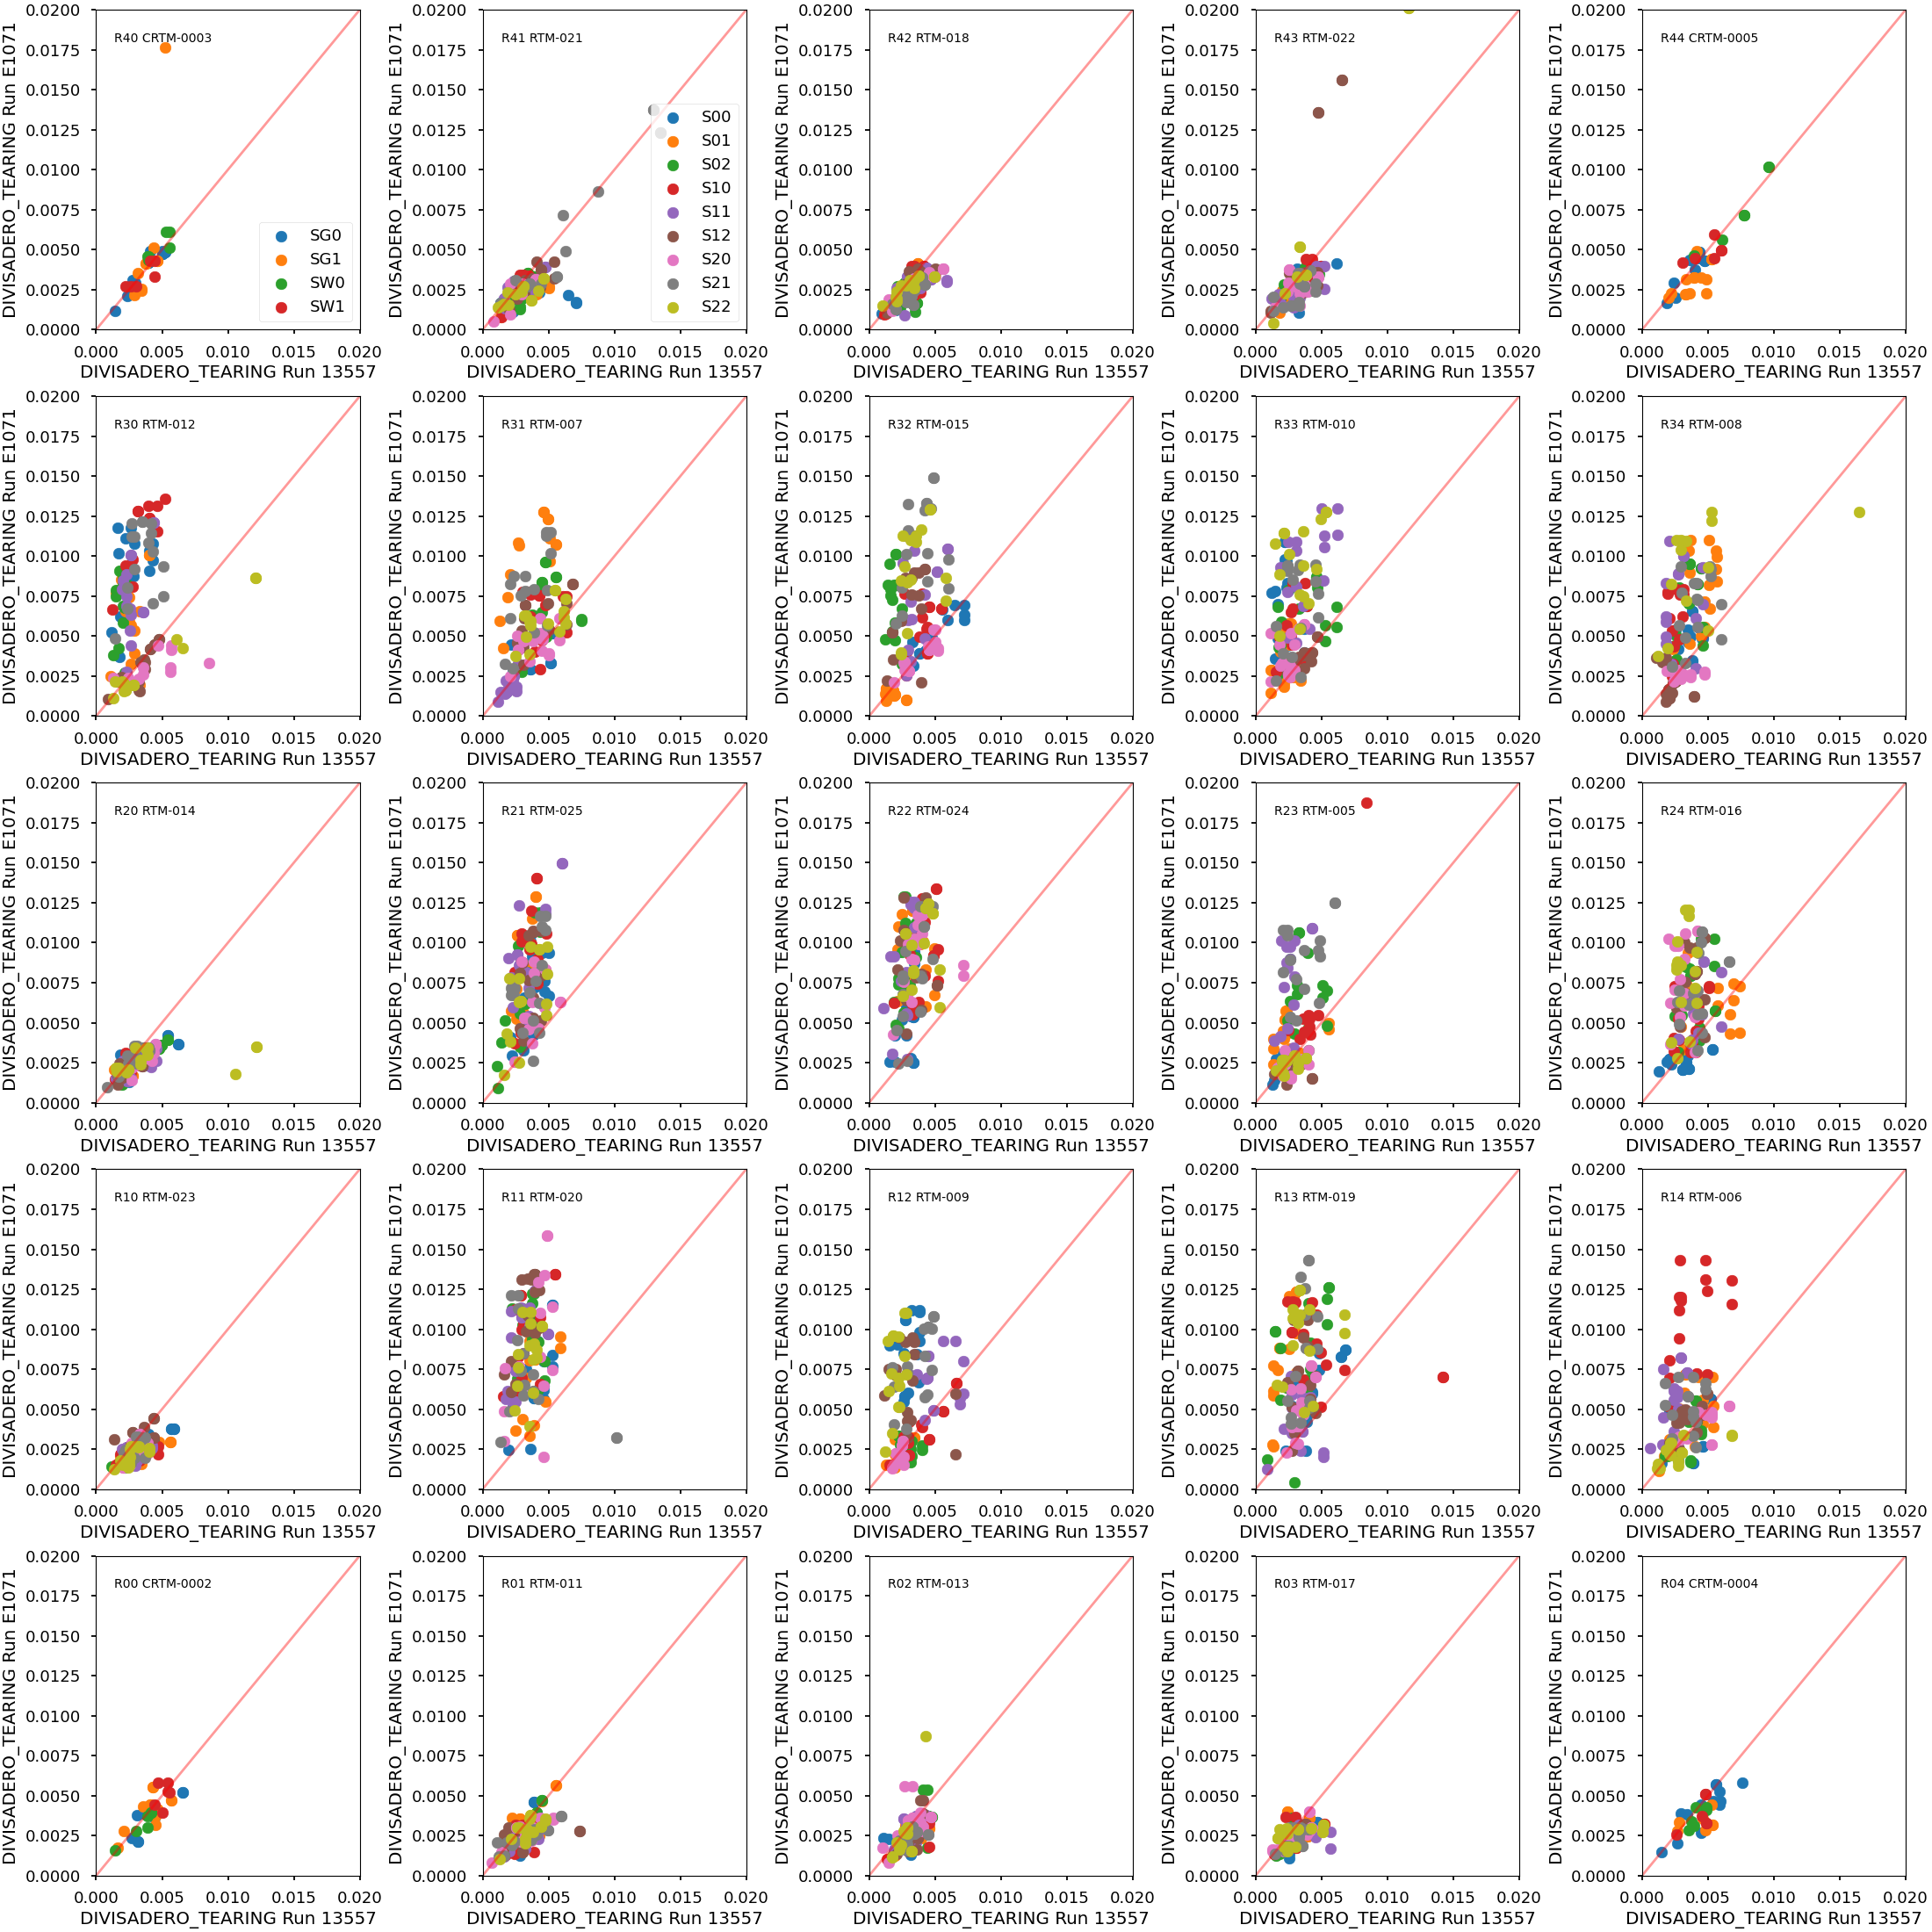
\includegraphics[width=0.7\textwidth]{sections/figures/baselineCharacterization/13557_E1071_DIVISADERO_TEARING.png}
\end{centering}
\end{figure}

Divisadero tearing in e2v CCDs is greater in Run 7 than in Run 6. The tearing signal in ITL
sensors is very consistent between Run 7 and Run 6, and much weaker than for e2v (Fig.~\ref{fig:divisadero}.

\begin{figure}[H]
\begin{centering}
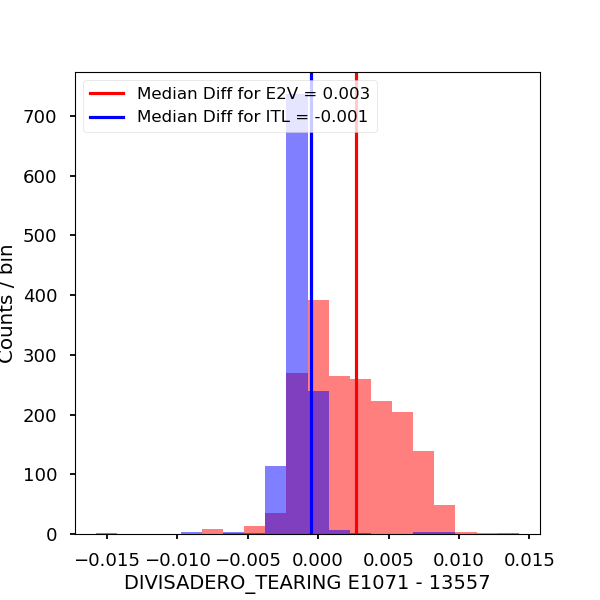
\includegraphics[width=0.7\textwidth]{sections/figures/baselineCharacterization/DIVISADERO_TEARING_13557_E1071_diff.png}
\caption{Distribution of difference between divisadero tearing in Run 7 (E1071) and Run 6 (13557), grouped by CCD type.}
\label{fig:divisadero}
\end{centering}
\end{figure}

In Run 7 the median divisadero tearing amplitude for e2v CCDs is \textasciitilde0.3\% greater. In ITL sensors, maximum divisadero tearing is \textasciitilde0.1\% greater in Run 6.

\subsubsection{Dark defects}\label{dark-defects}

Dark defects are localized regions or individual pixels that produce abnormally low signal levels, even in the presence of light. Similar to bright pixels, dark pixels are also quantified in dark columns over 50 pixel contiguous regions. These
defects are caused by imperfections in the semiconductor
material, imperfections during the manufacturing process of a CCD. For our evaluation, we extract
dark pixels from combined flats, with the threshold for a dark defect
defined as a $-$20\% deficit from the average flux measured in the image segment.

\begin{figure}[H]
\begin{centering}
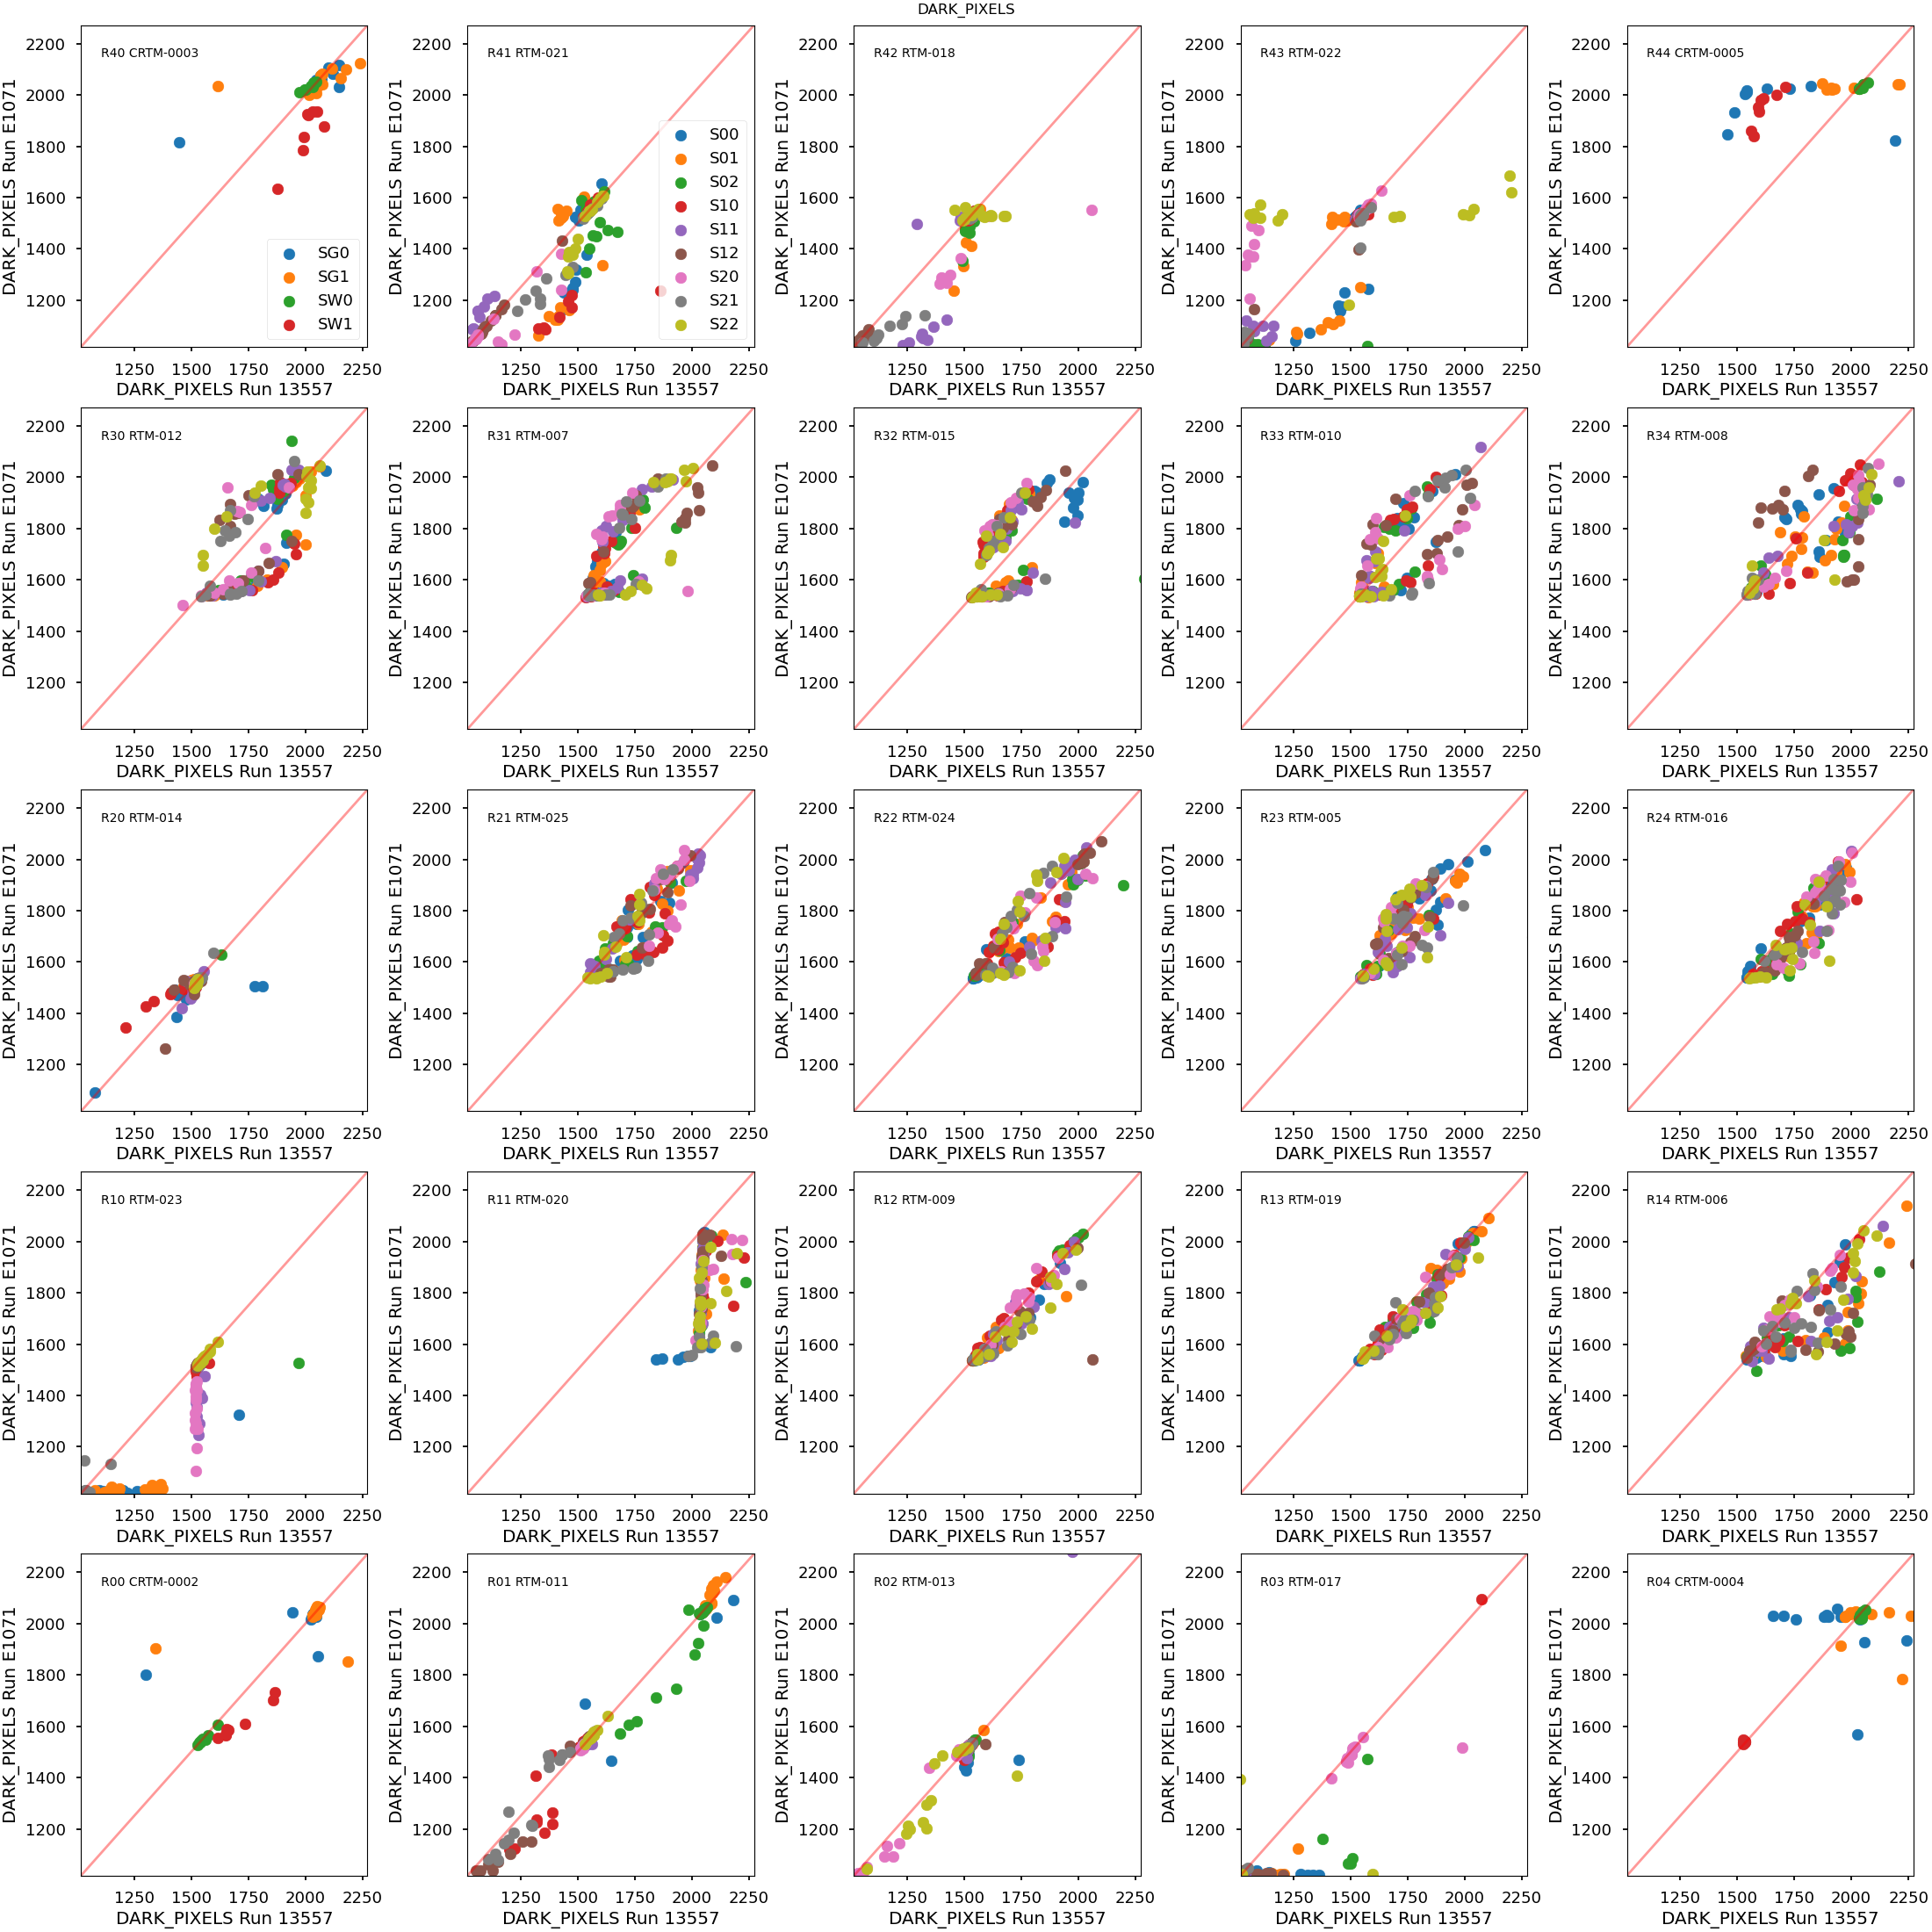
\includegraphics[width=0.7\textwidth]{sections/figures/baselineCharacterization/13557_E1071_DARK_PIXELS.png}
\caption{Comparison of dark pixel counts in Run 7 (E1071) and Run 6 (13557), with separate plots for each raft.  Within each plot the color coding for all amplifier segments in a given CCD is the same.}
\label{fig:dark-pixels}
\end{centering}
\end{figure}

Dark pixel counts measured in both Run 6 and Run 7 average
\textasciitilde1800 per amplifier (i.e., approximately 1M pixels), regardless of manufacturer. The
high dark pixel counts are due to the `picture-frame response' (also called `edge roll-off') 
near the edges of the amplifier segments.  The correlation between Run 7 and Run 6 dark pixel counts by CCD (Fig.~\ref{fig:dark-pixels}) is generally good, with some notable exceptions...

\begin{figure}[H]
\begin{centering}
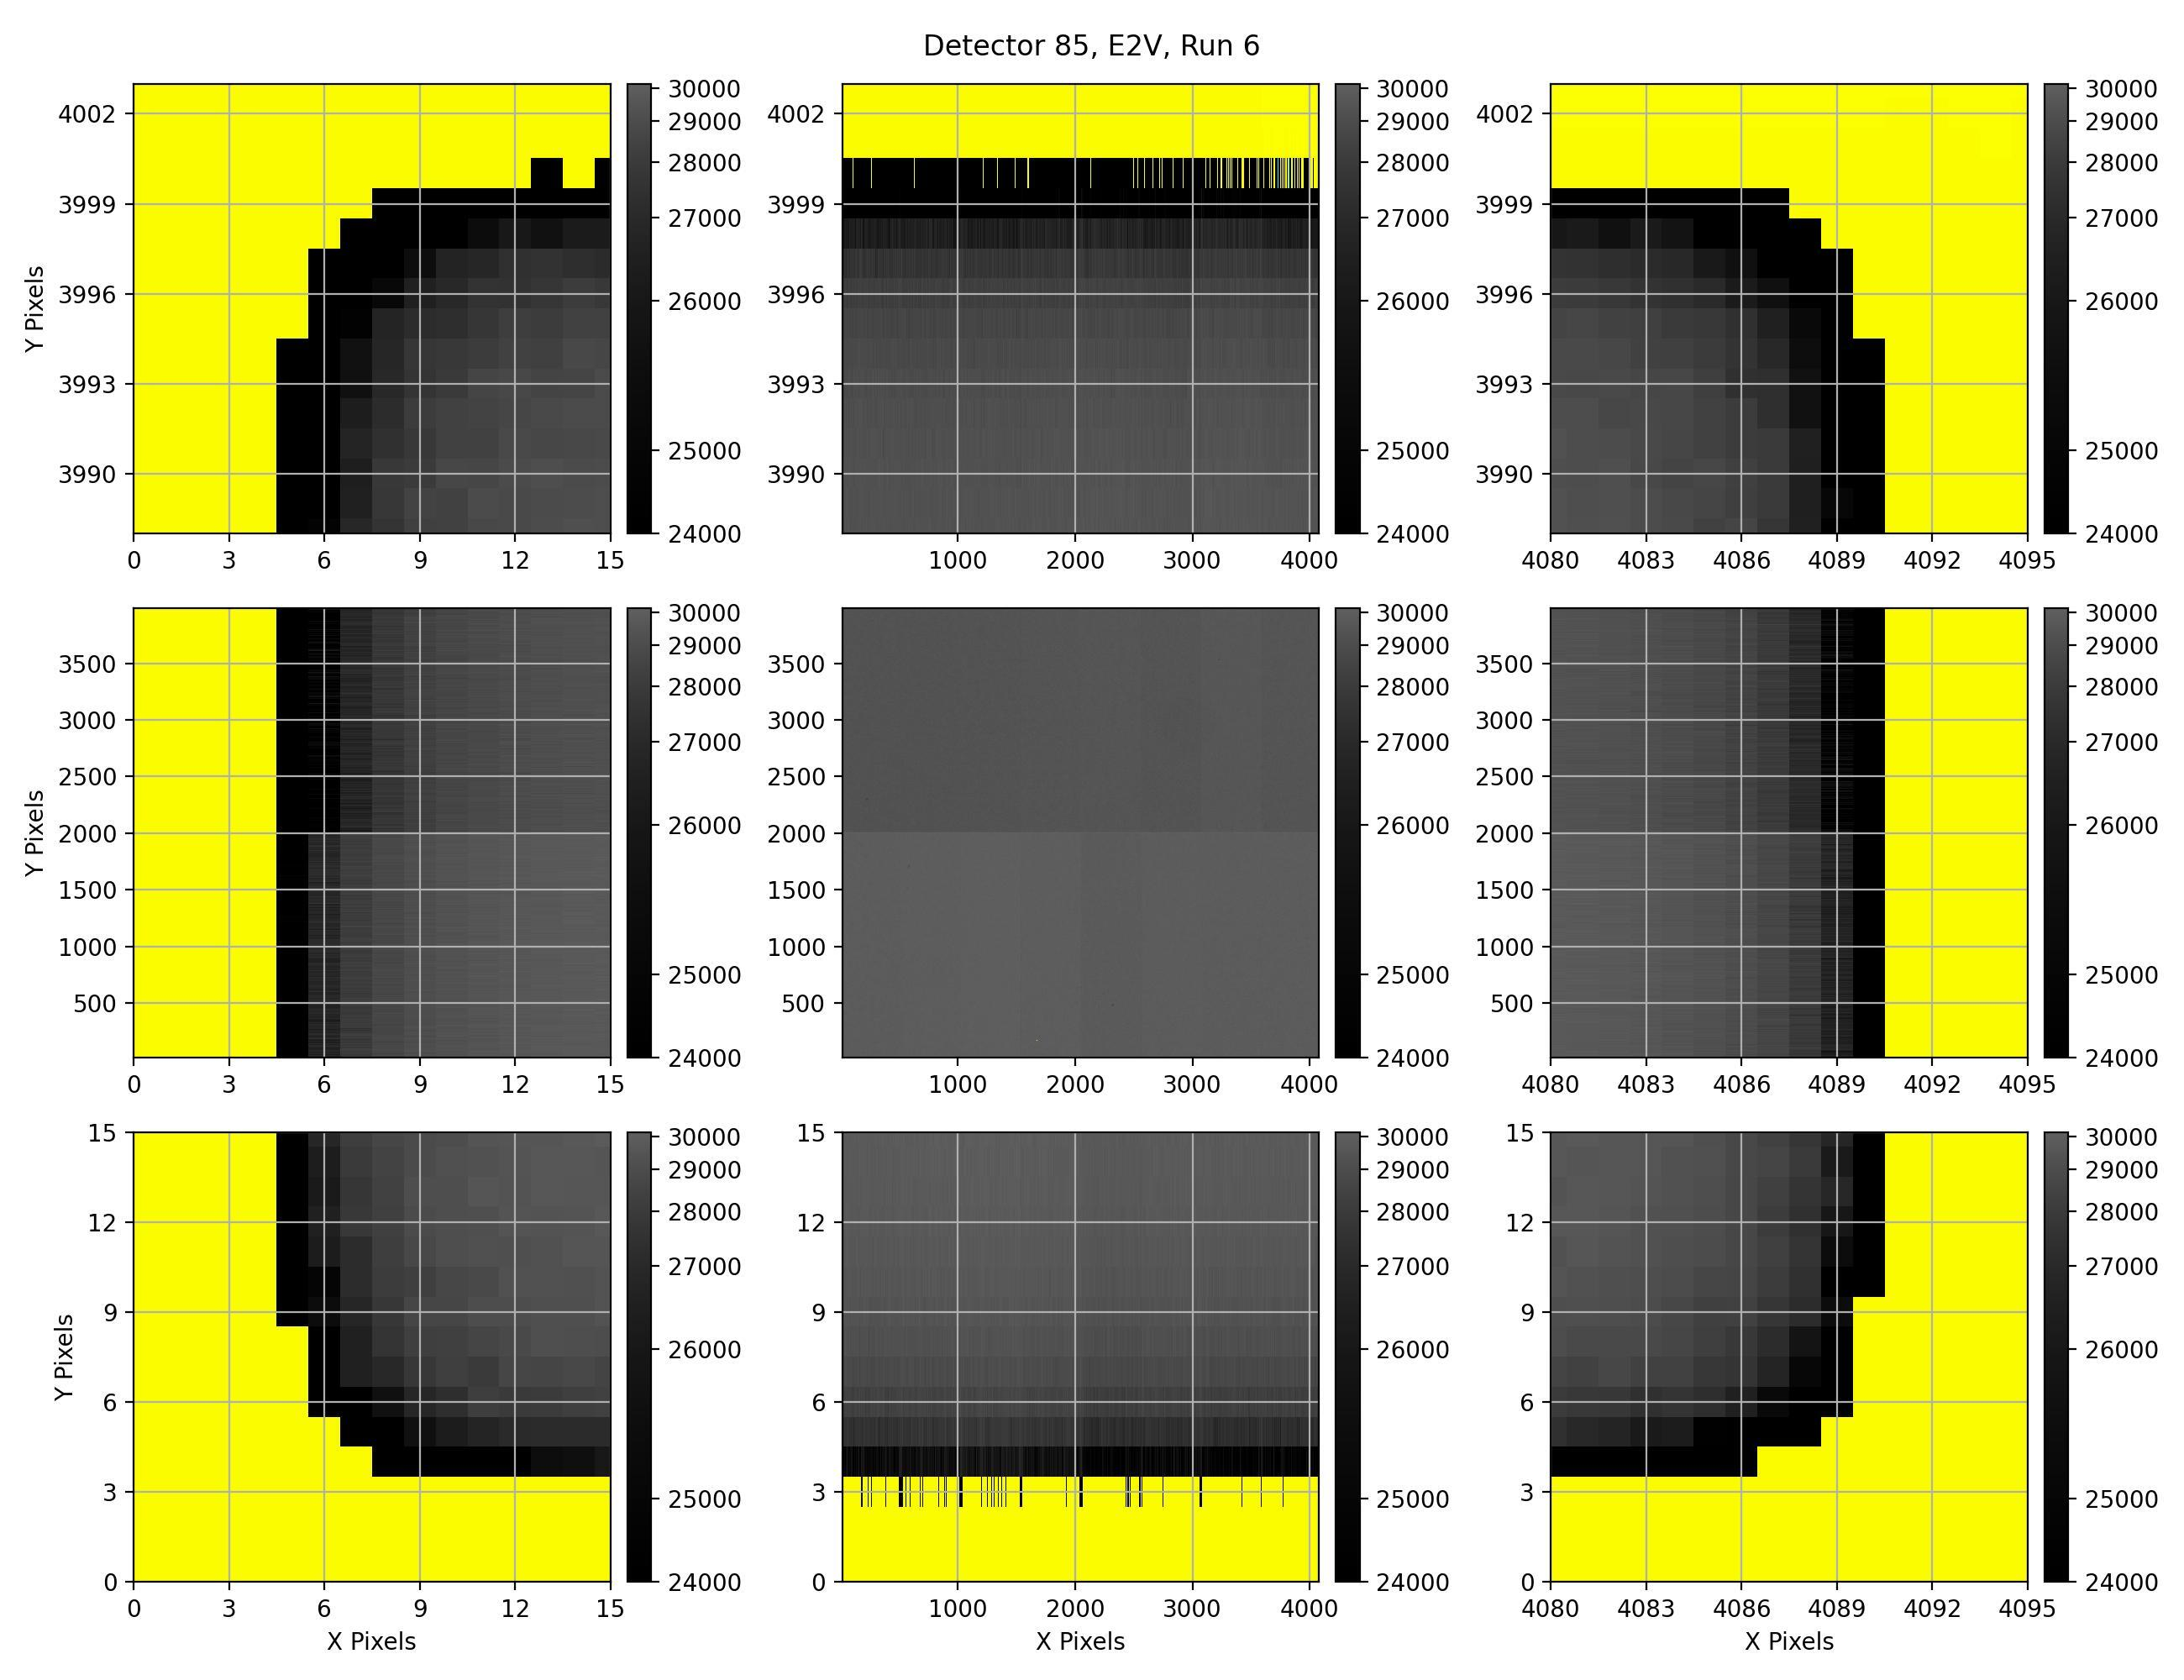
\includegraphics[width=0.7\textwidth]{sections/figures/baselineCharacterization/detector_85.jpg}
\end{centering}
\end{figure}

The eo-pipe defect configuration for evaluating dark defects considers a border pixel
region that is masked differently from the dark pixels. The default size for this edge is zero pixels. Due to the inclusion of the picture-frame response in the counts, it is difficult to
extract useful information about the dark defects in the focal plane. The default
configuration has no border masking. The largest region allowed for the
picture frame region is 9 pixels, determined by LCA-19363. Due to incompatibility of Run 6 data with the current pipelines, a direct comparison of a 9 pixel mask using Run 6 data is not currently available. However, a 9
pixel mask can be applied to the Run 7 data.

Add conclusion when pipelines on E1071 are complete

\subsection{Persistence}\label{persistence}

Persistence is a feature of CCDs and how they are operated involving charge trapped in the
surface layer after high-flux exposures
\hyperref[persistence-2]{{[}Persistence{]}}. Persistence is described in
detail in the
\href{https://sitcomtn-148.lsst.io/\#persistence-optimization}{persistence
optimization section}. Here we consider the measurements taken as
part of a persistence measurement task in the typical B protocol. For a
persistence measurement, a high-flux acquisition is taken, followed by a
sequence of dark images. The persistence signal has been observed to
decrease in subsequent dark images as the trapped charge is released. As a metric for persistence,
we evaluate the difference between the residual ADU in the first dark
image and the average of the residual ADU in the final dark images. This residual signal \textasciitilde10 ADU.

\begin{figure}[H]
\begin{centering}
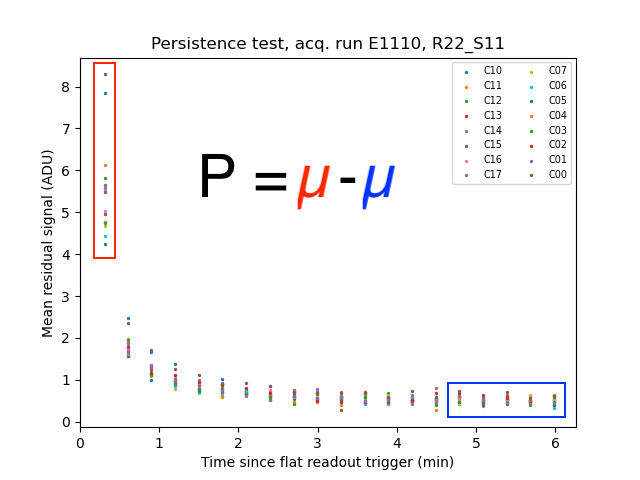
\includegraphics[width=0.7\textwidth]{sections/figures/baselineCharacterization/persistence_plot_LSSTCam_R22_S11_u_lsstccs_eo_persistence_E1110_w_2024_35_20240926T235141Z.png}
\end{centering}
\end{figure}

In the initial Run 7 measurements, we had not changed any operating
parameters of LSSTCam, so we would expect persistence to still be
present images at the same level as in Run 6.

\begin{figure}[H]
\begin{centering}
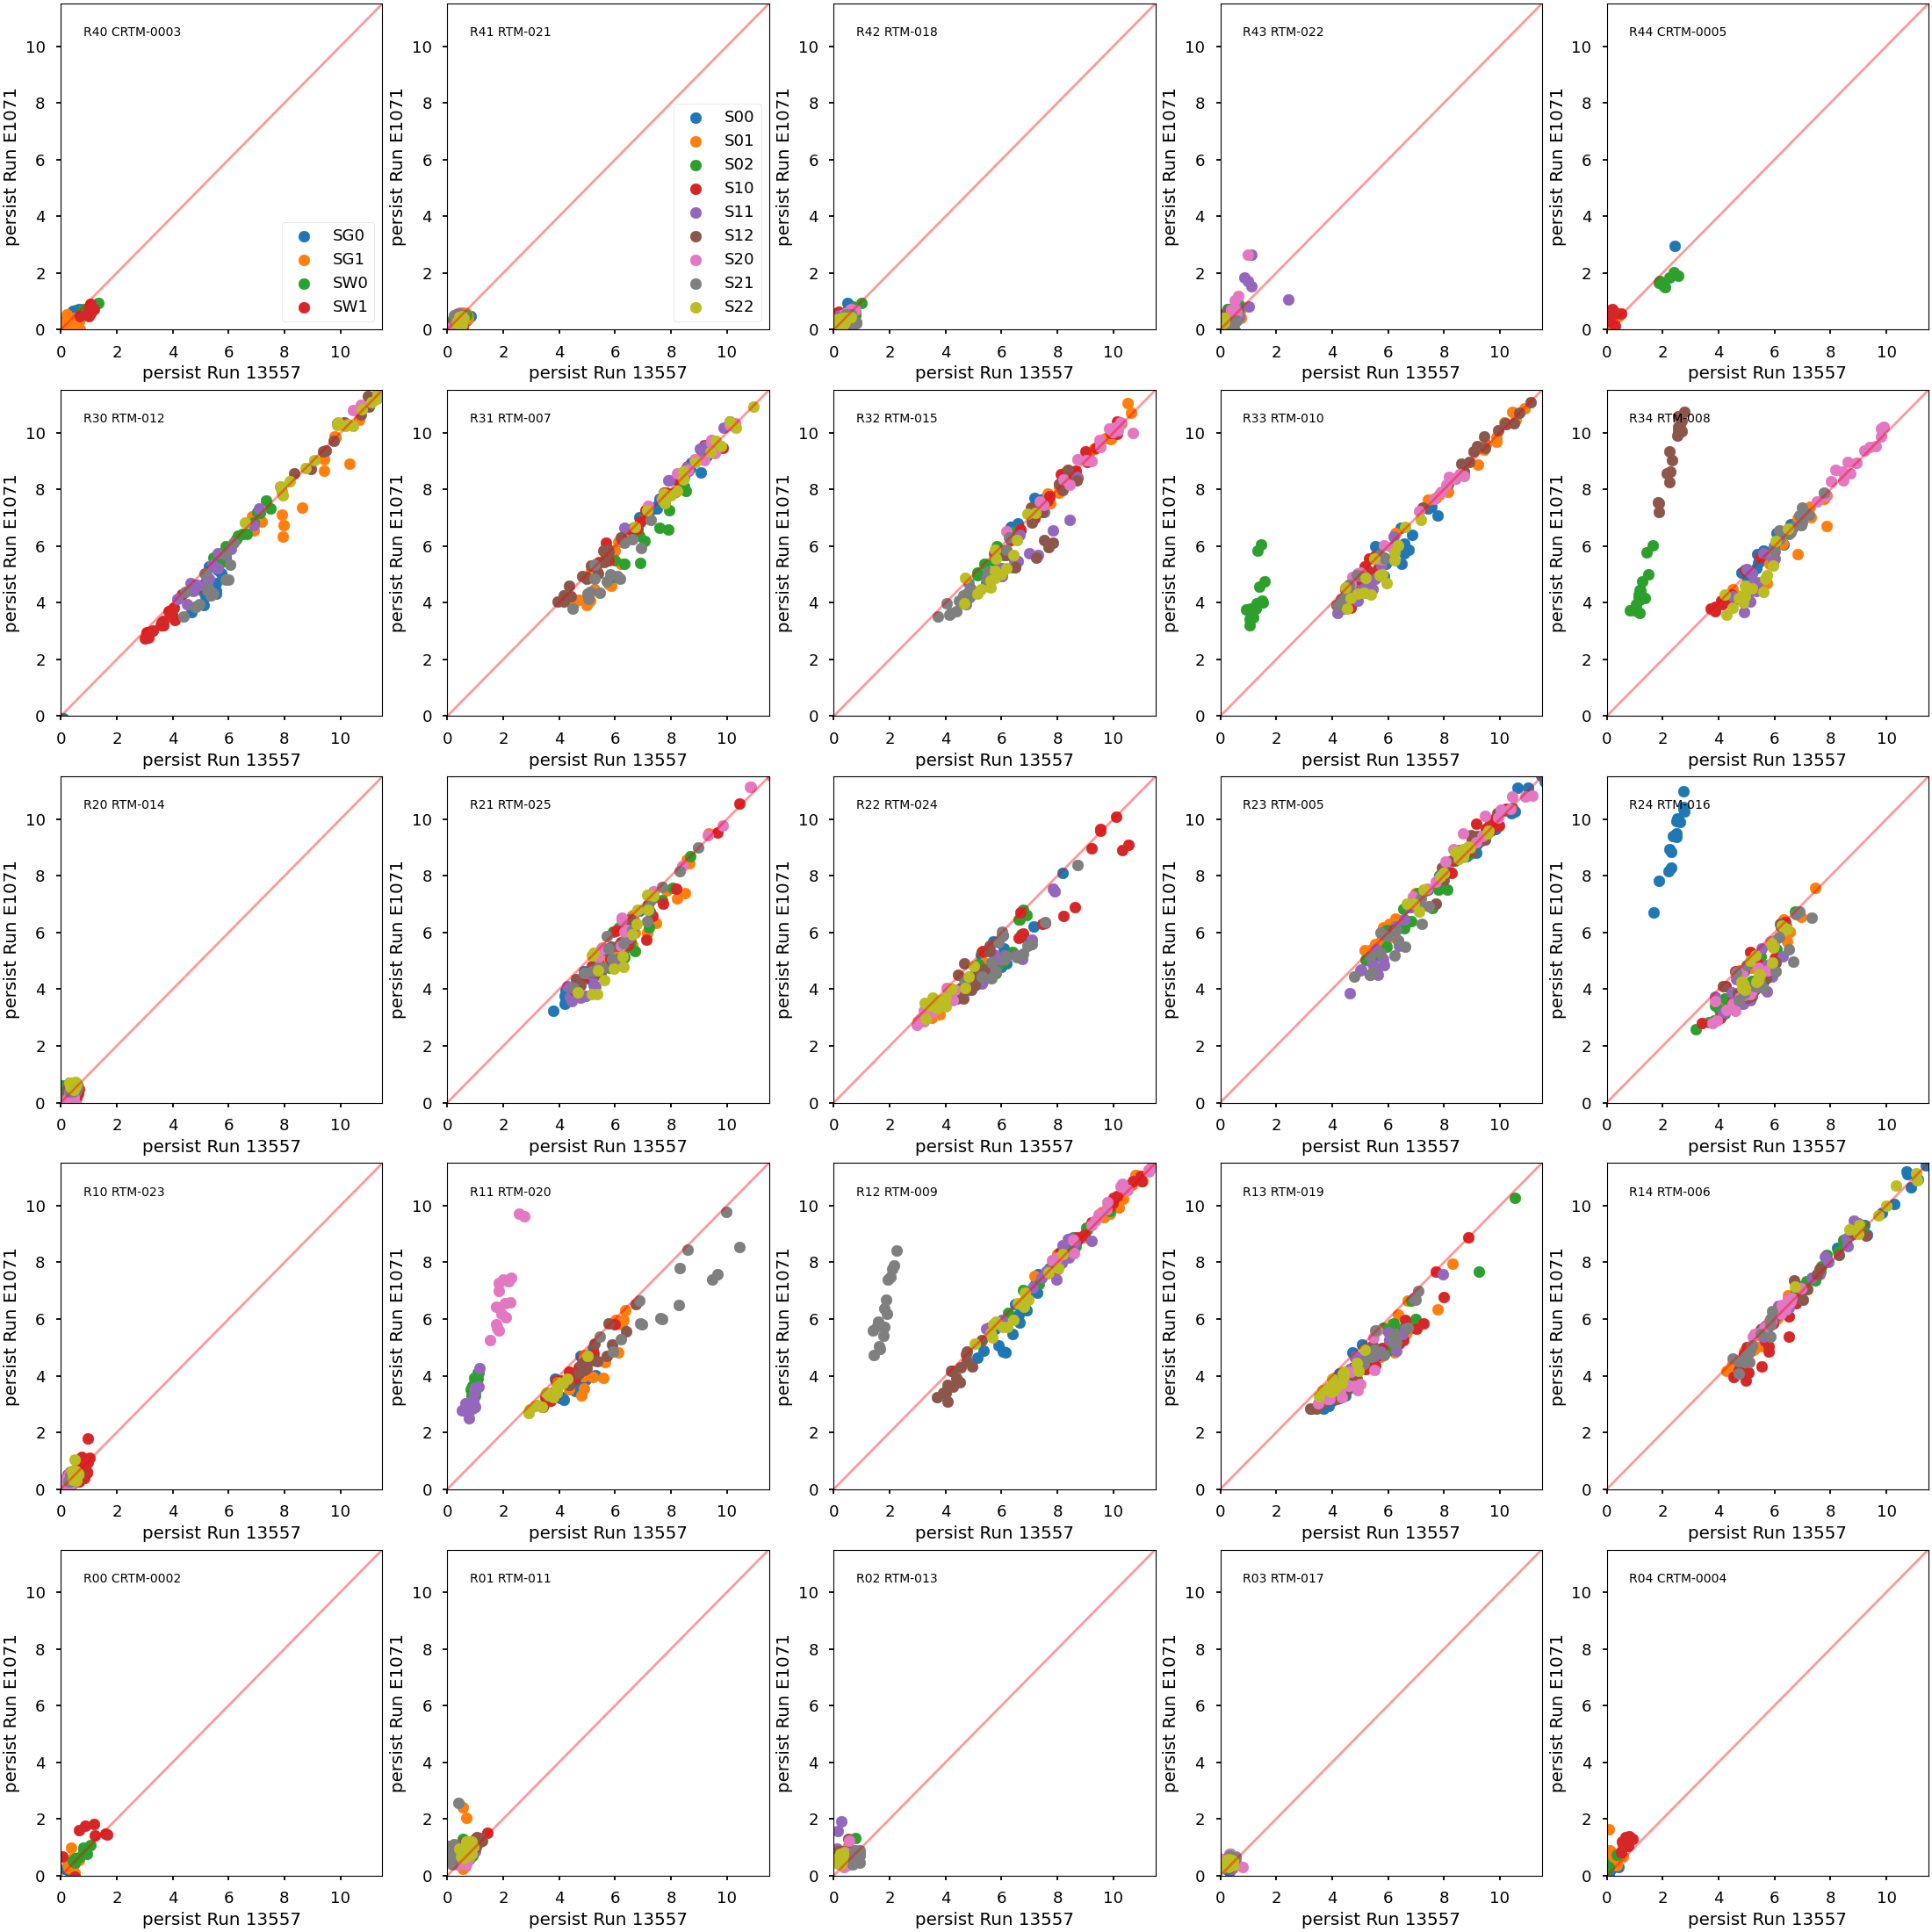
\includegraphics[width=0.7\textwidth]{sections/figures/baselineCharacterization/13557_E1071_persist.png}
\end{centering}
\end{figure}

The persistence signal is consistent in e2v sensors between Run 6 and Run 7. Several
outliers exist with higher persistence signal in Run 7. The outliers in
these measurements are due to higher initial persistence signal
measurements, resulting in an excess of \textasciitilde5 ADU when
comparing Run 6 with Run 7.

\begin{figure}[H]
\begin{centering}
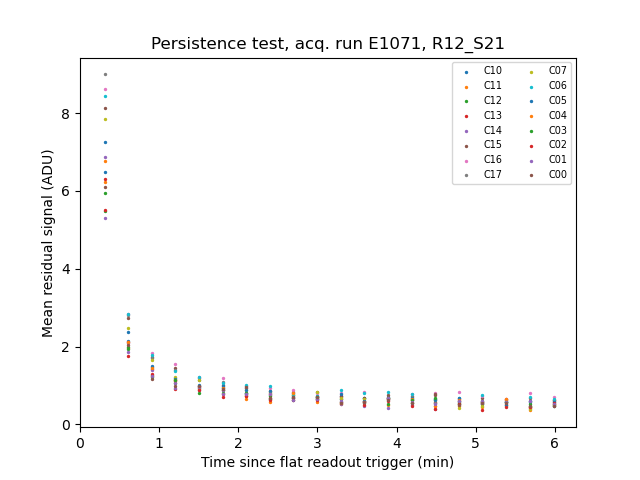
\includegraphics[width=0.7\textwidth]{sections/figures/baselineCharacterization/persistence_plot_LSSTCam_R12_S21_u_lsstccs_eo_persistence_E1071_w_2024_35_20240925T180602Z.png}
\end{centering}
\end{figure}

\begin{figure}[H]
\begin{centering}
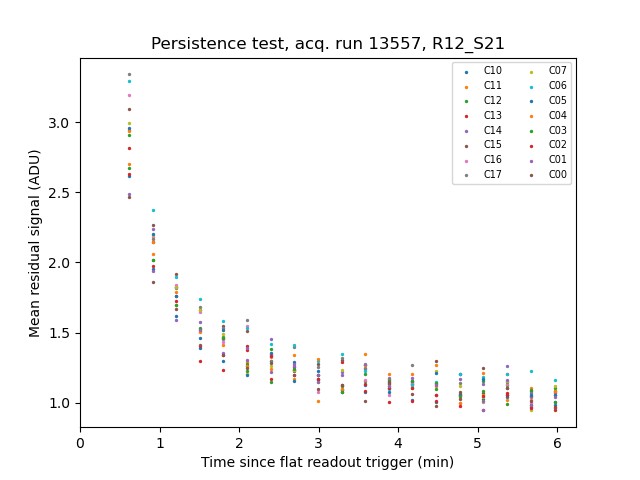
\includegraphics[width=0.7\textwidth]{sections/figures/baselineCharacterization/persistence_plot_LSSTCam_R12_S21_u_lsstccs_eo_persistence_13557_w_2023_41_20231118T050437Z.png}
\end{centering}
\end{figure}

\subsection{Differences between run 6 and run 7}\label{differences-from-previous-runs}

% Add something about the major differences between the runs

% Please add the following required packages to your document preamble:
% \usepackage{multirow}
\begin{table}[H]
\begin{tabular}{|l|ll|ll|}
\hline
\multirow{2}{*}{Parameter [unit]}          & \multicolumn{2}{l|}{E2V}                   & \multicolumn{2}{l|}{ITL}                    \\ \cline{2-5} 
                                    & \multicolumn{1}{l|}{Run 6}     & Run 7     & \multicolumn{1}{l|}{Run 6}     & Run 7      \\ \hline
Serial CTI {[}\%{]}                 & \multicolumn{1}{l|}{3.6816E-7} & 1.1357E-7 & \multicolumn{1}{l|}{1.5922E-6} & 1.6478E-6  \\ \hline
Parallel CTI {[}\%{]}               & \multicolumn{1}{l|}{1.2162E-7} & 1.0554E-7 & \multicolumn{1}{l|}{1.6931E-8} & -4.7849E-8 \\ \hline
Dark current {[}e-/pix/s{]}         & \multicolumn{1}{l|}{}          &           & \multicolumn{1}{l|}{}          &            \\ \hline
Bright defects {[}count{]}          & \multicolumn{1}{l|}{}          &           & \multicolumn{1}{l|}{}          &            \\ \hline
Linearity turnoff {[}e-{]}          & \multicolumn{1}{l|}{112410.98} & 112162.66 & \multicolumn{1}{l|}{105960.37} & 106002.95  \\ \hline
PTC turnoff {[}e-{]}                & \multicolumn{1}{l|}{90422.94}  & 89697.03  & \multicolumn{1}{l|}{78209.44}  & 77913.08   \\ \hline
PTC Gain {[}e- / ADU{]}             & \multicolumn{1}{l|}{1.4785}    & 1.4811    & \multicolumn{1}{l|}{1.6717}    & 1.6760     \\ \hline
PTC $a_{00}$ [$\frac{1}{pix^2}$]      & \multicolumn{1}{l|}{3.0854E-6} & 3.0863E-6 & \multicolumn{1}{l|}{1.7119E-6} & 1.7031E-6  \\ \hline
BF x-correlation                    & \multicolumn{1}{l|}{0.5236}    & 0.5169    & \multicolumn{1}{l|}{0.7155}    & 0.7521     \\ \hline
BF y-correlation                    & \multicolumn{1}{l|}{0.1785}    & 0.1707    & \multicolumn{1}{l|}{0.2859}    & 0.2869     \\ \hline
Row-means variance                  & \multicolumn{1}{l|}{0.9927}    & 0.8836    & \multicolumn{1}{l|}{0.9924}    & 0.9466     \\ \hline
Dark defects {[}count{]}            & \multicolumn{1}{l|}{}          &           & \multicolumn{1}{l|}{}          &            \\ \hline
Divisadero tearing maximum {[}\%{]} & \multicolumn{1}{l|}{}          &           & \multicolumn{1}{l|}{}          &            \\ \hline
Persistence {[}ADU{]}               & \multicolumn{1}{l|}{}          &           & \multicolumn{1}{l|}{}          &            \\ \hline
\end{tabular}
\end{table}


\section{Camera Optimization}\label{camera-optimization}

\subsection{Persistence optimization}\label{persistence-optimization}

Leftover signal (``persistence") in the first dark image acquired after intense illumination has
been observed.  Persistence has been observed
in an early prototype e2v sensor as early as 2014
\hyperref[D2014]{{[}D2014{]}}. It was confirmed that the amplitude of
the persistence decreased as the parallel swing voltage was decreased.
This is consistent with the effect being a residual surface image
\hyperref[J2001]{{[}J2001{]}}, i.e., the excess charges are being held
at the surface layer. The level of persistence is about 10--20 ADU,
and the decay time constant is about 30\,s
\hyperref[dmtn-276]{{[}dmtn-276{]}}.

During the EO testing in 2021, we also found the persistence made a
streak toward the readout direction from the place where a bright spot illumination occurred 
in a previous image. We call this ``trailing persistence".

As noted in Section (ref. tearing section above), depending on operating conditions e2v sensors have another major non-ideality, so-called ``tearing", which is
considered a consequence of the non-uniform distribution of holes. Over the past few years, our
primary focus in the optimization of the operating parameters was mitigation of the tearing, and we successfully eliminated the tearing by changing the
e2v voltages from unipolar (both parallel rails high and low
are positive) to bipolar (the parallel high is positive, and
the low is negative) following the formula
\hyperref[Bipolar]{{[}Bipolar{]}}. However, the persistence issue
remained unchanged.

For the persistence issue, if this is a residual surface image, two
approaches could be taken as discussed in \hyperref[U2024]{{[}U2024{]}}:  
either 1) establishing the pinning condition where the holes make a thin
layer at the front surface so that the excess charges recombine with
the holes, or 2) narrowing the parallel swing so that the accumulated
charges in the silicon do not get close to the surface state.

The pinning condition could be established by decreasing the parallel low
voltage to as low as -7\,V or lower. The transition voltage needs to be
empirically determined. However, Teledyne e2v advised that the measured
current flow increases as the parallel low voltage is decreased, which
increases the risk of damaging the sensor by inducing a
breakdown\footnote{We note that ITL operates at a parallel low voltage
  of -8.0\,V. We have observed the increased current flow. But we have
  software protection so that the current does not increase too much.}.
Also, the excess charges could be recombined by the thin layer of
the holes, which could affect linearity at high flux levels when
charges start to interact with the holes.

The parallel swing determines the full-well. Depending on whether the
accumulated charges spread over the columns or interact with the surface
layer, there are blooming full-well regimes and the surface full-well
regime. A full-well level between these two regimes is considered to be
optimal \hyperref[J2001]{{[}J2001{]}}, with no persistence and and dynamic range as great as
possible. Because we observe the persistence effect, we likely operate the sensor in the
surface full-well condition and we need to decrease the parallel swing to
get the blooming full-well or the optimal full-well. The obvious downside
decreasing the full-well capacity.

The sensor control voltages are defined relative to each other. Changing, e.g., the parallel
swing also requires changes to all other voltages to
operate the sensor properly, e.g., to properly reset the amplifier.
The initial voltages were given in the original formula
\hyperref[Bipolar]{{[}Bipolar{]}} but to decrease the parallel swing we had
to switch to the new formula in order to satisfy the constraints
\hyperref[PersistenceMitigationVoltage]{{[}PersistenceMitigationVoltage{]}}.

\hyperref[S2024]{{[}S2024{]}}, set up a single sensor test-stand at UC
Davis. They attempted multiple different approaches mentioned above and
reported the results \hyperref[DavisReport]{{[}DavisReport{]}}. The
summary is as follows:

\begin{itemize}
\tightlist
\item
  The new voltages following the rule work fine.
\item
  Narrowing the parallel swing eliminates the persistence.
\item
  Lowering the parallel low voltage did not work
  as we expected; going to a more negative voltage is probably needed.
\end{itemize}

Note that the e2v sensor in the UCD setup did not exhibit persistence.
This might be due to the characteristics of the sensor, or perhaps
the differences in the electronics (e.g., the long cable between CCD and REB). They need to move the parallel rails up.

\subsubsection{Persistence
optimization}\label{persistence-optimization-1}

Based on this test result, we decided to test the new voltages with
the narrower parallel swing on the LSSTCam focal plane. Keeping the
parallel low voltage at -6\,V in order to operate the sensor safely (very
conservative limit), we changed the parallel swing voltage from 9.3\,V to
8.0\,V as well as all the other voltages using the new formula. We
overexposed the CCDs and took 20 darks afterward. The image shown below is the
mean and median of pixel-by-pixel differences between the first and the
last dark exposures, as a function of the parallel swing. As the
parallel swing is decreased, the residual signal decreases, reaching
roughly 10$\times$ less than the original level at 9.3\,V. Although we sampled
midpoints between 8.0 and 9.3\,V, 8.0\,V appears to work the best and could
be lower with the penalty of decreasing the full-well capacity.

\begin{figure}
\begin{centering}
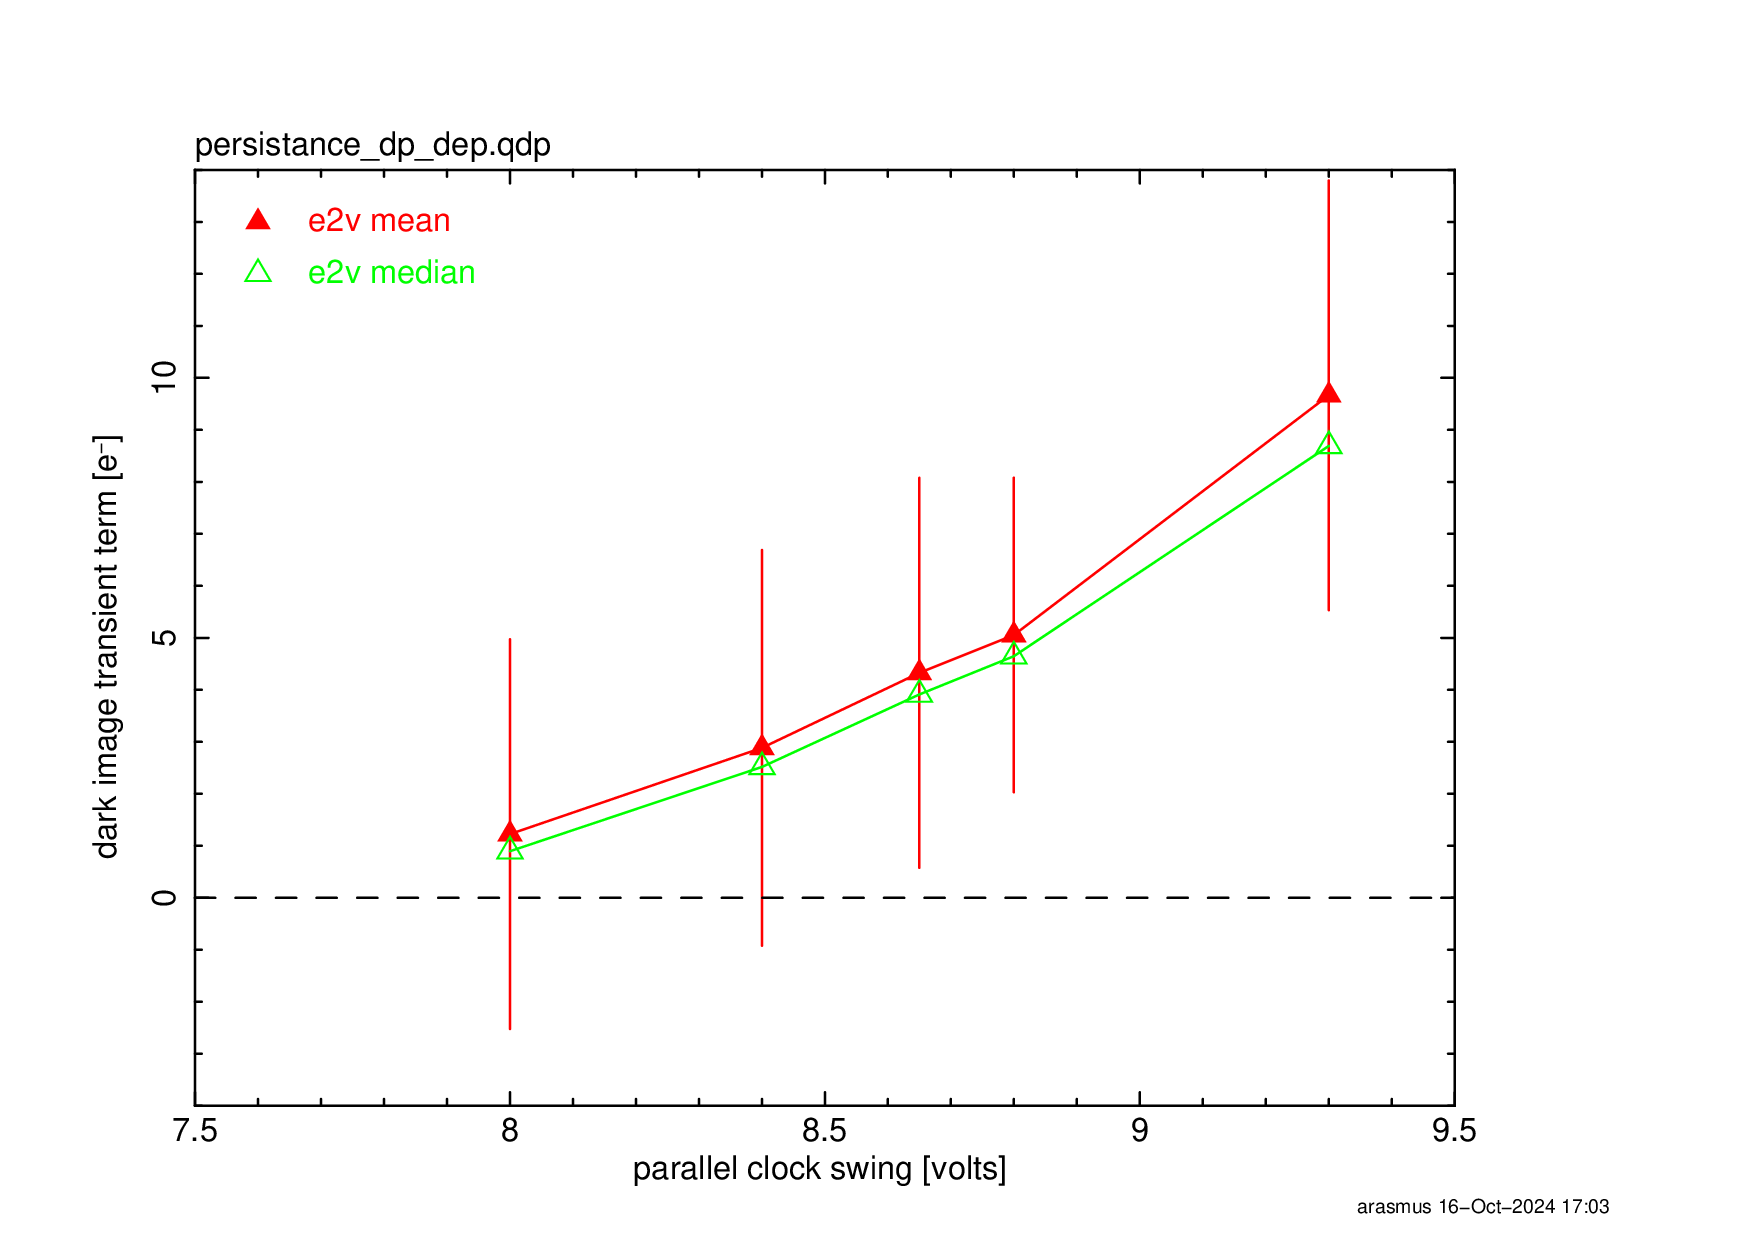
\includegraphics[width=0.9\textwidth]{sections/figures/e2v_transient_dark_vs_dp.png}
\end{centering}
\caption{The remaining charges measured in every amplifier but
aggregated by mean and median as a function of the parallel clock swing
are shown.}
\end{figure}

The following figures display how the persistence is reduced by the
parallel swing decrease. The images were processed with the standard instrumental
signature removal and assembled in the full focal-plane view. The
dark exposure was taken right after a 400\,ke-equivalent flat exposure.
The figure shows the distinct pattern of elevated signal associated with
the e2v sensors, which fill the inner part of the focal plane.

The right-hand figure shows the same dark exposure but taken with the narrow
parallel swing voltage of 8.0\,V. The distinct pattern goes away. This
demonstrates the persistence in e2v sensors becomes the (low) level of the 
ITL sensors.


\begin{figure}[h]
\centering
\begin{minipage}[b]{0.45\textwidth}
\centering
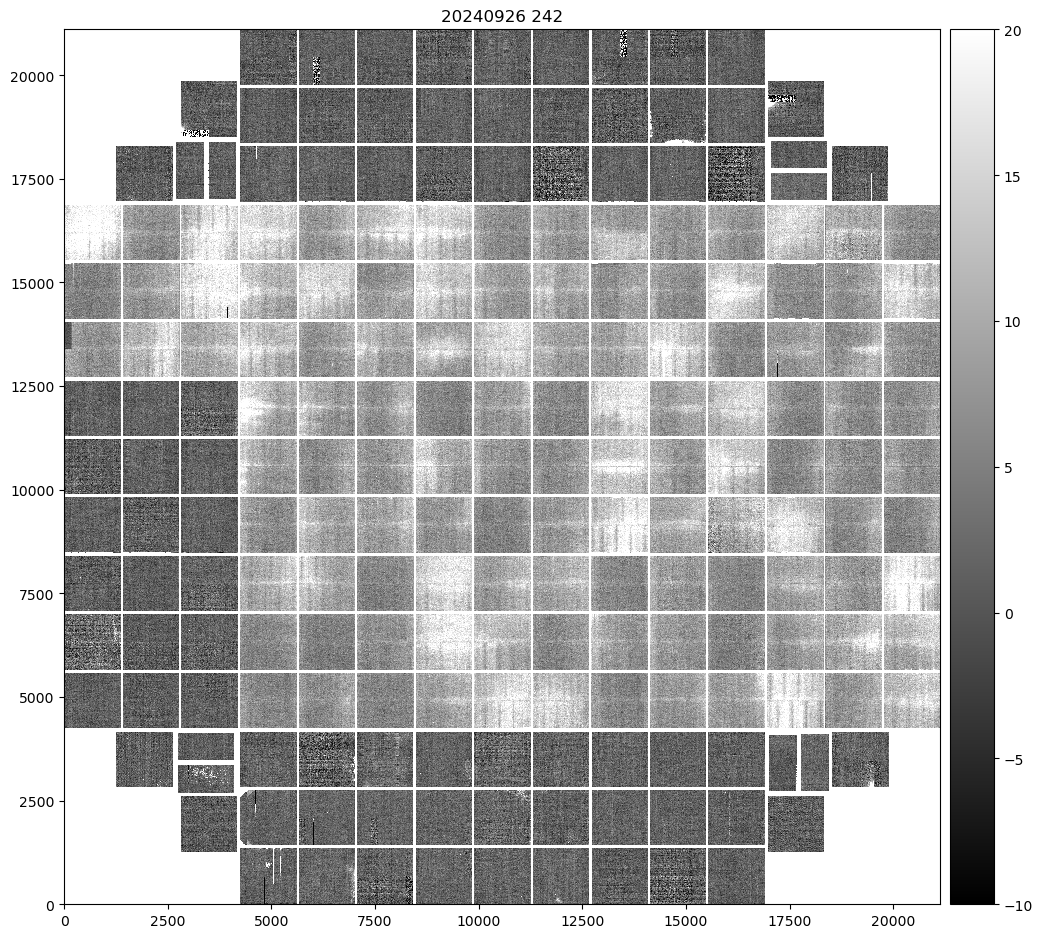
\includegraphics[width=\textwidth]{sections/figures/E1110dp93.png}
\end{minipage}
\hfill
\begin{minipage}[b]{0.45\textwidth}
\centering
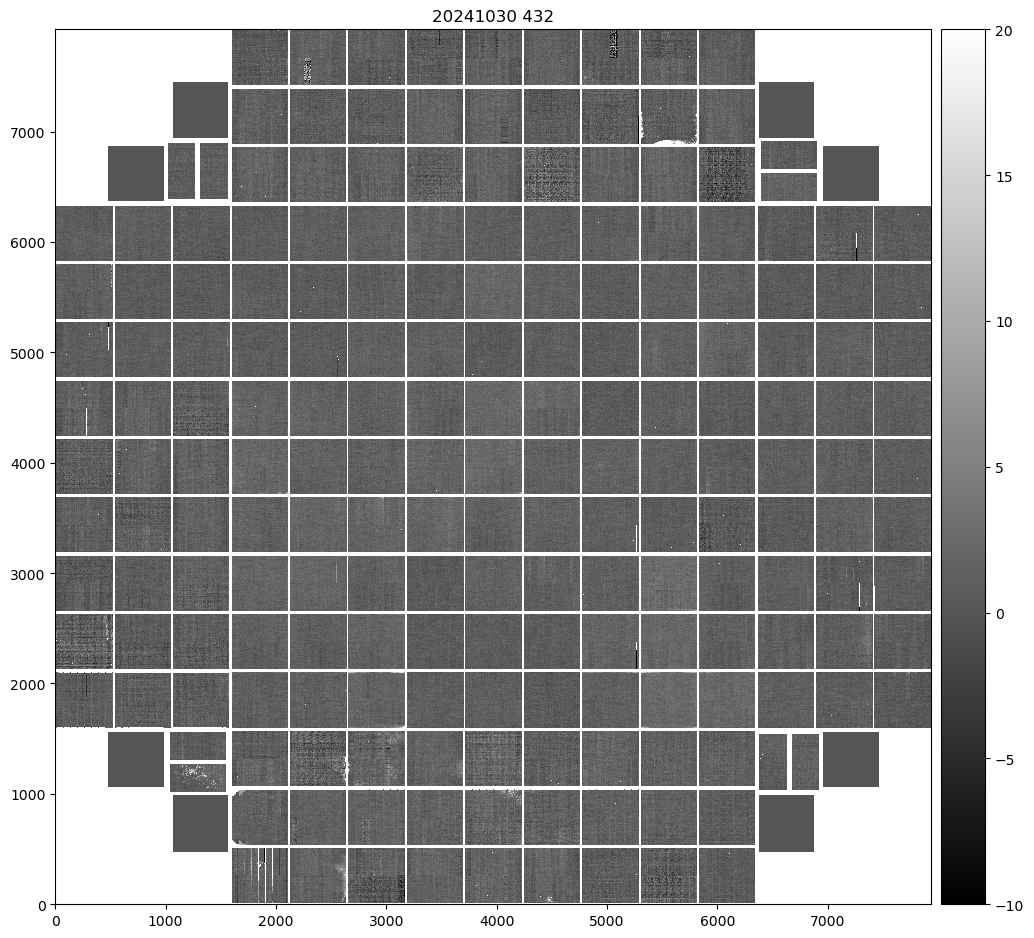
\includegraphics[width=\textwidth]{sections/figures/E1880dp80.png}
\end{minipage}
\caption{Comparison of dark exposures under different parallel swings. (left) The first dark exposure after a 400\,ke$^-$ flat image under the parallel swing of 9.3\,V (Run E1110); (right) The first dark exposure after a 400\,ke$^-$ flat image under the parallel swing of 8.0\,V (Run E1880). The figure shows no distinct patterns from persistence in e2v sensors. Note that the guide sensors were not displayed here because they were being operated in guider mode. Also some of the residuals in ITL caused by defects disappeared here because of the employment of the new sequencer file (v30).}
\end{figure}



\subsubsection{Impact on full-well}\label{impact-on-full-well}

Reduction of the full well is expected from narrowing the parallel swing
voltage. This subsection explores how much reduction in the PTC turnoff
is observed in the dense PTC runs. Two runs were acquired with identical
setting except for the CCD operating voltage (E1113 for 9.3\,V and E1335
for 8.0\,V). As the PTC turnoff is defined in ADU, it needs to be
multiplied by PTC\_GAIN to compare the turnoff values in electrons.
The figure below compares the PTC turnoffs in electrons and also shows their
fractional difference. The median reduction was 22\%.

\begin{figure}
\begin{centering}
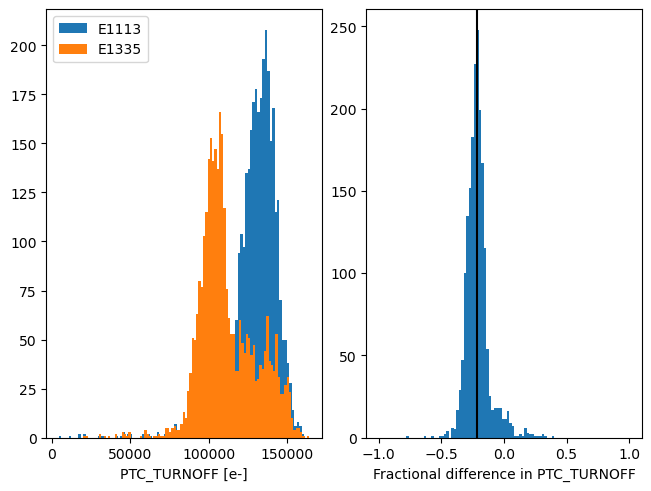
\includegraphics[width=0.9\textwidth]{sections/figures/PtcTurnoffRatio.png}
\end{centering}
\caption{Histograms of the PTC turnoff values scaled to electron units (left) and the ratios of
differences (right) between E1113 (9.3\,V) vs E1335 (8.0\,V). The median of
the reduction is 22\%.}
\end{figure}



\subsubsection{Impact on brighter-fatter
effect}\label{impact-on-brighter-fatter-effect}

Reducing the parallel swing is expected to enhance the brighter-fatter
effect (BFE), possibly in an anisotropic way. The BFE can be
characterized via the evolution of the variance and covariances of
flat field exposures as a function of flux, i.e., via a PTC analysis. To evaluate the
impact of reducing the parallel voltage swing on e2v sensors, we
acquired two series of flat field exposures with the respective voltage
setups and extracted the ``area" coefficients 
(Equation (1) in \hyperref[A2023]{{[}A2023{]}}). The area coefficients describe by how much a unit charge stored in
a pixel will alter the area of some other pixel (or itself). We find that
reducing the parallel swing from 9.3\,V to 8.0\,V typically increases the
area coefficients by 10\% (between 5 and 19\% depending on distance),
and the increase is almost isotropic (i.e., very similar along serial and parallel
directions). From these measurements, we anticipate that the increase of
star sizes with flux in LSST data will not become more isotropic at 8.0\,V than it was at
9.3\,V, and hence this reduction of parallel swing does not 
%introduce new threats on the measurement of the PSF ellipticity
risk increasing systematic uncertainty of the PSF ellipticity.

\begin{figure}
\begin{centering}
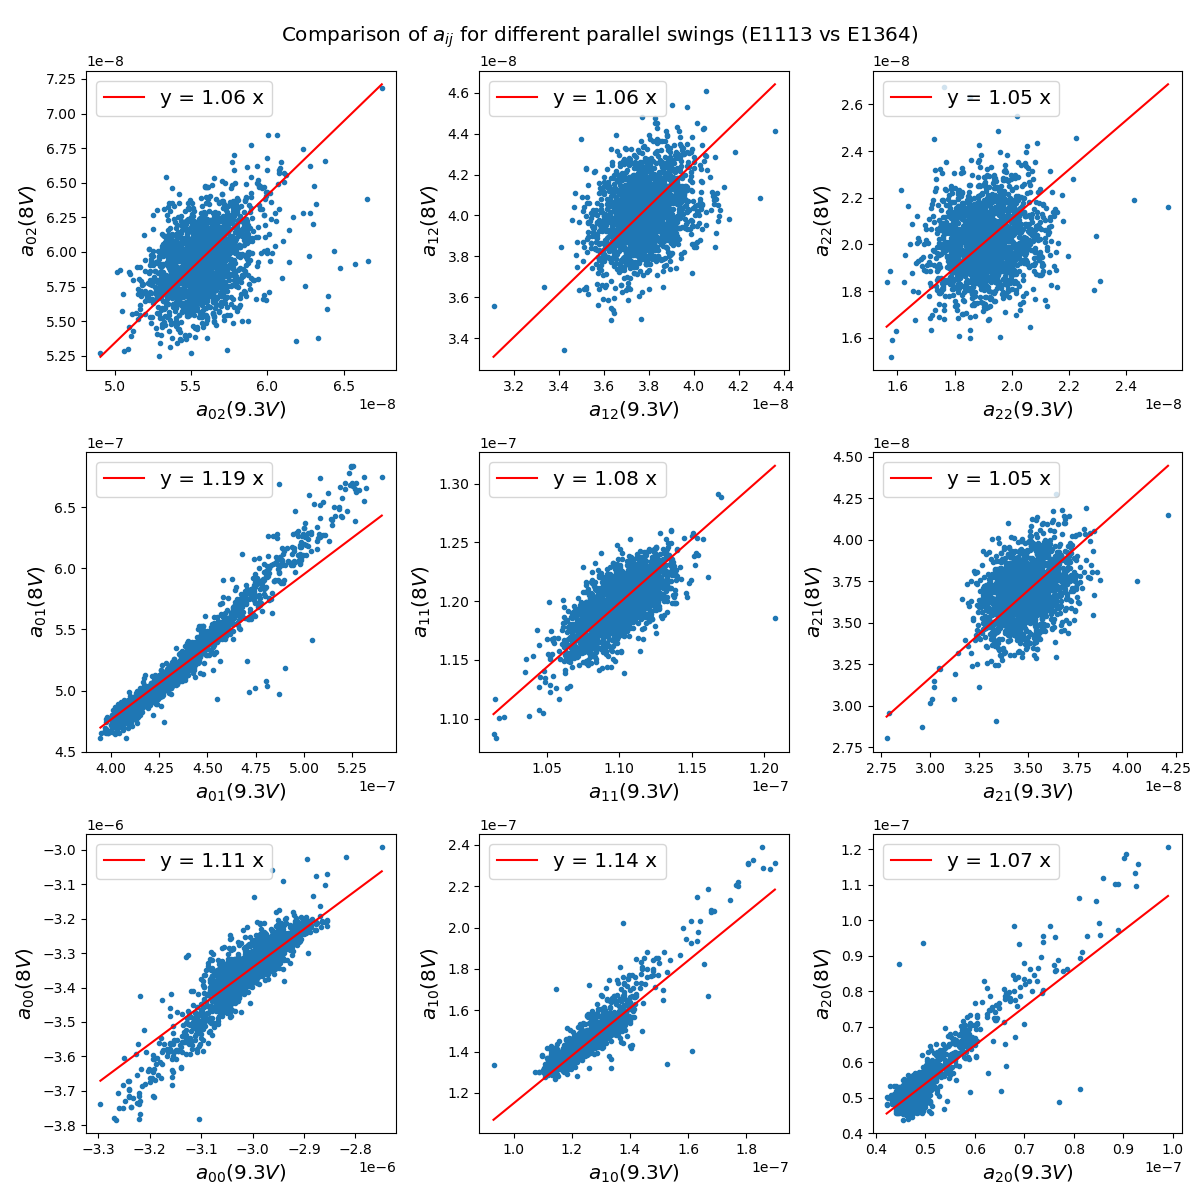
\includegraphics[width=0.8\textwidth]{sections/figures/aScatterPlots8vs9-3.png}
\end{centering}
\caption{Scatter plots of area coefficients $a_{ij}$(one entry per amplifier)
measured at 8.0\,V and 9.3\,V. The sub-figures correspond to separations in rows ($j$) and columns ($i$)
between the source of the area distortion and its victim, with the self
interaction coefficient $a_{00}$ at the bottom left. The first neighbors increase
respectively by 19\% in the parallel direction by 14\% in the serial
direction. So the BFE is slightly larger at 8.0\,V but not significantly
more anisotropic.}
\end{figure}


\subsection{Sequencer Optimization}\label{sequencer-optimization}



Several efforts were undertaken to optimize the sequencer configurations during Run 7. The following points summarize the key investigations:

\begin{itemize}
\item Clears:  Here we summarize the discussion provided in
  \href{https://sitcomtn-148.lsst.io/\#serialRemnants}{Improvement of
  Clear CCD}:

  \begin{itemize}
  \item
    \textbf{No Pocket}
  We introduced the V29\phantomsection\label{nop}{NoP} (No Pocket)
  sequencer, which is an improved clear method using a serial register
  configuration that reduces the formation of pockets at the Image/Serial
  register interface. This clear method showed an approximately 2$\times$
  improvement in the saturated image clear for e2v devices and completely
  resolved the issue for ITL devices, except for R01\_S11,
  where the No Pocket method performs approximately 2x worse than the default clear. 
  For an unknown reason, this ITL CCD retains a significant amount of uncleared charges 
  (hundreds of lines) after a saturated flat. This issue prevents the use of the No
  Pocket configuration with ITL devices.

  \item
    \textbf{No Pocket with Serial Flush}
  We introduced V29NoPSF (No Pocket with Serial Flush), an enhanced version of the No Pocket Clear
  sequencer, which includes a variable configuration of the serial register
  during the clear process (mimicking a serial flush), to further prevent the
  formation of pockets. This solution has been shown to completely prevent the presence of leftover charges after clearing a saturated image for e2v devices.
  \end{itemize}
  

\item Phase overlap during parallel transfer for e2v: e2v sensors feature four parallel phases. To improve the uniformity of the full well across a sensor, overlapping two phases during each time slice of the parallel transfer was introduced. However, this overlap is known to cause trailing persistence, as reported in \ref{DavisReport}. We conducted several runs using both intermediate overlapping and non-overlapping sequencers. By optimizing the operating voltages to avoid charge trapping, the trailing persistence is no longer a concern.
\end{itemize}

\subsection{Improved Clear}\label{improved-clear}

\subsubsection{Overview}\label{overview}

In this section, we describe the work done during Run 7 to improve
the image clear prior to collecting a new exposure.

The problem we wanted to address is the presence of residual charges in
the first lines read for an image taken just after the clear of a saturated
image. These ``hard to clear" charges are associated with highly
saturated flats or columns (or stars as observed in AuxTel or ComCam),
which leave signal in the first lines of the subsequent exposure. The effect has a sensor-specific signature:

\begin{itemize}
\item
  In all ITL CCDs (except in R01\_S10 for which
  the effect is much more significant and which will be addressed later
  in this section):

  \begin{quote}
  The first CCD line of an exposure read after an image with saturated
  overscan is close to saturation and in most of cases a small leftover signal is also present in the second line.
  \end{quote}
\item
  In e2v CCDs:

  \begin{quote}
  Although the effect is slightly amplifier dependent, as for ITL, the
  first line read after an exposure that follows an exposure with saturated
  overscan, is close to saturation, and a significant signal is visible
  in the subsequent 20--50 lines. (
  \texttt{see\ left\ plots\ of\ clear\ e2v\ image\textless{}fig-image-e2vclear\textgreater{}})
  \end{quote}
\end{itemize}

These leftover electrons are not associated with what we usually call 
residual image or persistence. They are suspected to be associated with
pockets, induced by the electric field configuration in the sensor and
the field associated with saturated pixels: pocket(s) that survive to a
clear, will prevent charges to be cleared. A change of the electric
field (e.g., a change in the configuration of the clocks) can remove the pockets, and
free the charges, allowing them to be cleared. If charges stuck in
pocket(s) are not removed by a clear, we observed that an additional image read
(e.g., a bias) will fully remove them: only the first exposure taken after
an image with saturated overscan is impacted. If the clocks
configuration used in our standard clear is not able to flush away those
charges, a standard readout of \textgreater\textasciitilde{} 2000 lines
does remove them.

The localization of these uncleared electrons in the first lines of the
CCDs, indicates that the interface between the image area and the serial register
is the location of the pockets. For this reason we investigated
changes in the field configuration of the serial register during the
clear, to avoid pockets at the image-serial register interface.

\subsubsection{New sequencers}\label{new-sequencers}

To address this clear issue, we focussed on updating the serial
register field as the lines are moved to it. The constraint being that
the changes introduced should not significantly increase the clear
execution time. It should be noted that in 2021 we tried =a sequencer
called ``Deep Clear" ( \hyperref[sequencerV23_DC]{{[}sequencerV23\_DC{]}}
) as a first attempt to address the clear issue: it added one full line
flush on top of the existing one at the end of the clear. This sequencer
did improve the clear, but did  not fully fix the clear issue (see
\texttt{Summary\ table\textless{}table-SummaryClear\textgreater{}}).

In Run 7, we considered on top of the default clear, two new
configurations. The changes are in the ParallelFlush function, which
moves the charges from the image area to the serial register:

\begin{itemize}
\tightlist
\item
  The default clear (V29): In the default clear, all serial clock voltages are
  kept up as the parallel clocks move charges from the image area to the
  serial register (\hyperref[sequencerV29]{{[}sequencerV29{]}}). The
  charges once on the serial register are expected to flow to the ground:
  the serial register clocks being all up, without pixel boundaries, and
  with its amplifier in clear state. At the end of the clear, a full
  flush of the serial register is done (\textasciitilde{} the serial
  clocks changes to read a single line).
\item
  The No-pocket Clear (NoP): a clear where the serial register has the
  same configuration (S1 \& S2 up, S3 low) when the parallel clock P1
  moves the charges to the serial register than in a standard image read. Still we kept all phases up for the rest of the time for a fast clear
  of the charges along the serial register
  (\hyperref[sequencerV29_NoP]{{[}sequencerV29\_NoP{]}}). The idea is
  that the S3 phase is not designed to be up when charges are transferred
  to the serial register, and is probably playing a major role in the creation of pockets.
\item
  The No-pocket with serial flush Clear (NoPSF): this sequencer is close
  to the NoP solution, except that during the transfer of one line to
  the serial register, the serial phases are also manipulated to transfer two
  pixels along the serial register. The changes in electric field at the
  image-serial register interface are then even more representative of
  what a standard read produces, and should further prevent the
  creation of pockets.
  (\hyperref[sequencerV29_NoPSF]{{[}sequencerV29\_NoPSF{]}}).
\end{itemize}

\subsubsection{Results on standard e2v and ITL CCDs}\label{results-on-standard-e2v-and-itl-ccd}

\begin{figure}
\begin{centering}
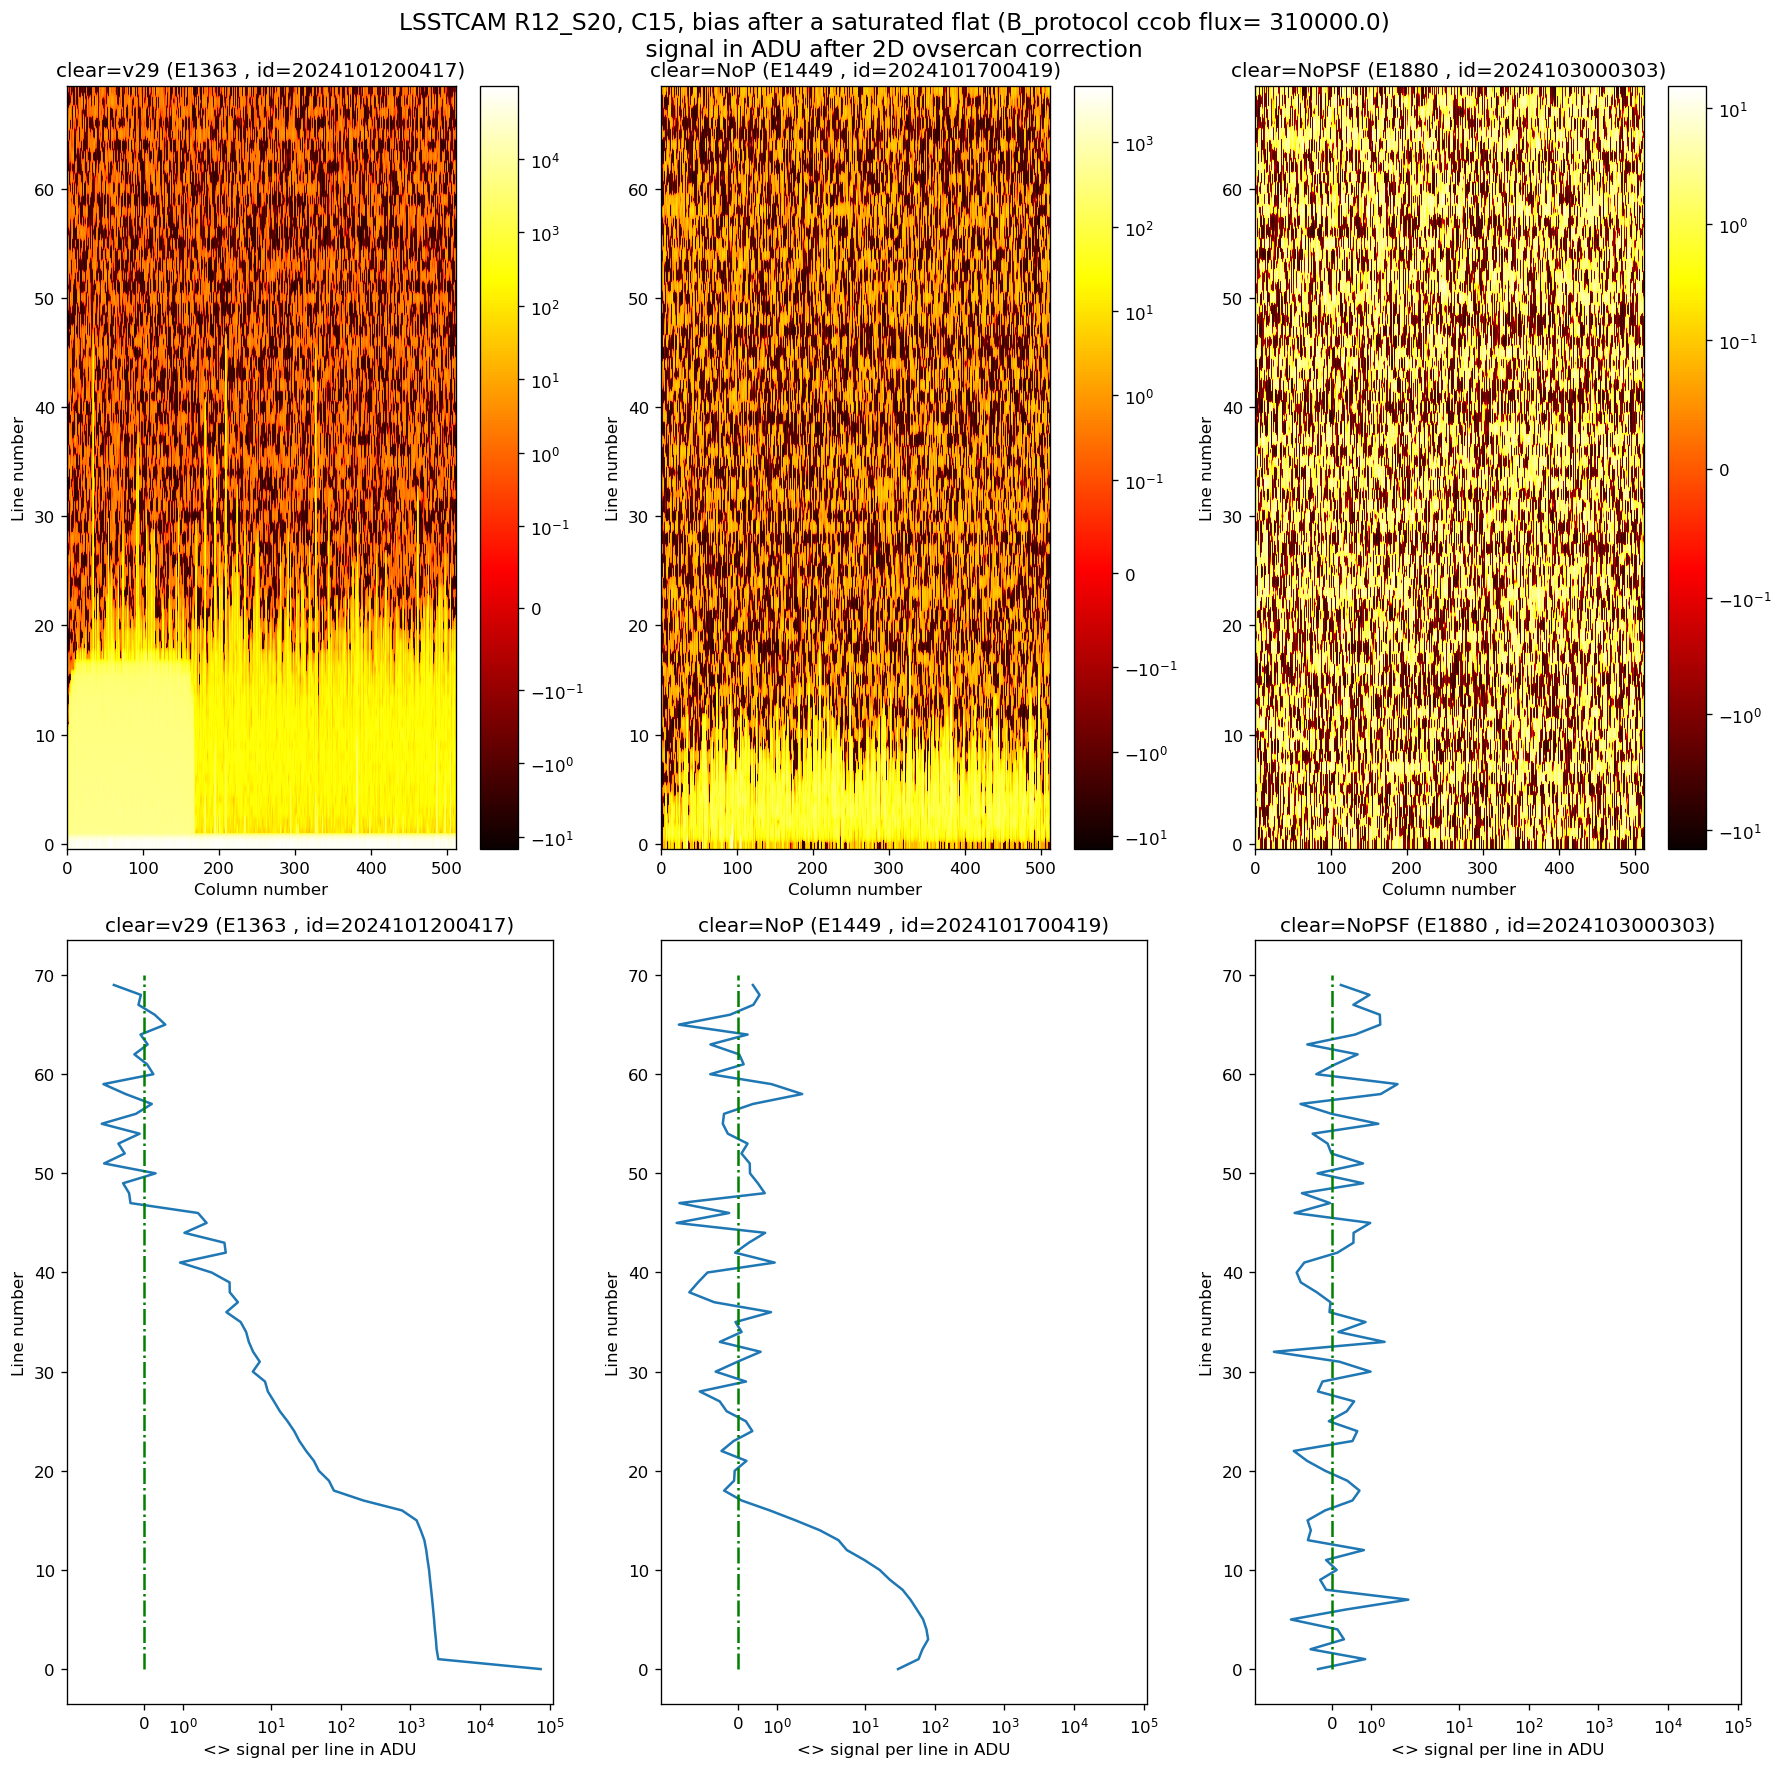
\includegraphics[width=0.9\textwidth]{sections/figures/plots_R12_S20_C15_E1880_bias_2024103000303.png}
\end{centering}
\end{figure}

\emph{Figure showing the impact of the various types of clear on a bias
taken after a saturated flat for an e2v sensor.}

\begin{figure}
\begin{centering}
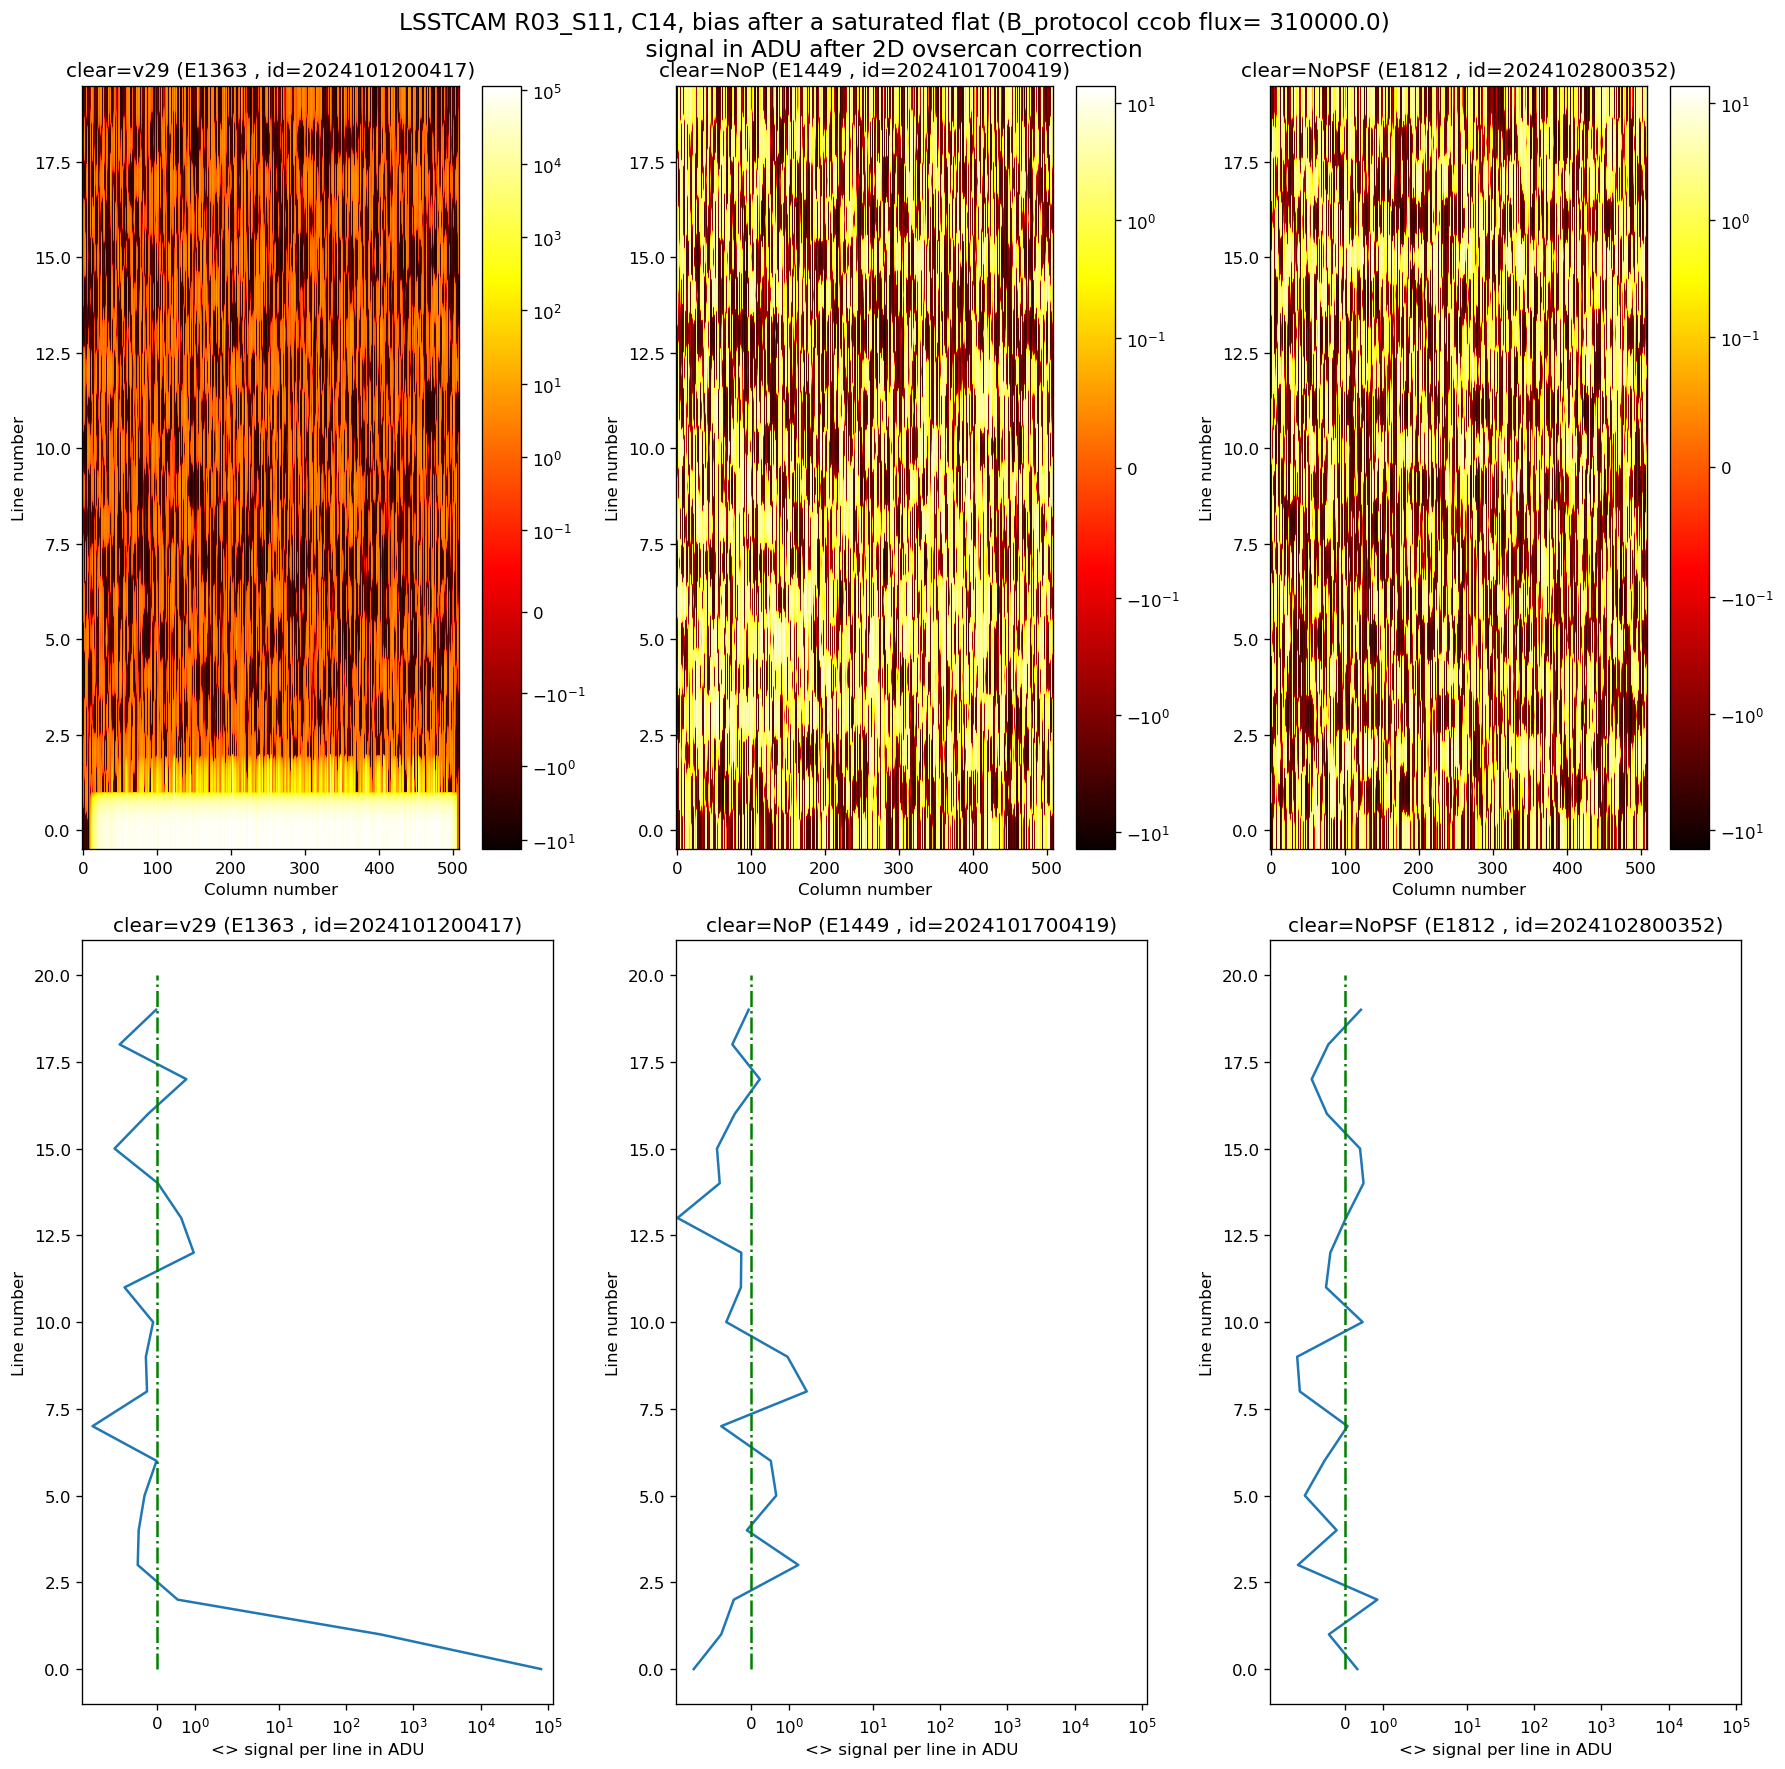
\includegraphics[width=0.9\textwidth]{sections/figures/plots_R03_S11_C14_E1812_bias_2024102800352.png}
\end{centering}
\end{figure}

\emph{Figure showing the impact of the various types of clear on a bias
taken after a saturated flat for an ITL sensor.}

In the above images, we present for three types of sequencer (from left to
right: V29, NoP, and NopSF), a zoom on the first lines of an ITL or e2v
amplifier (for ITL R03\_S11\_C14 and for e2v
R12\_S20\_C10 shown as a 2D lines-columns
image (top plots) or as the mean signal per line for the first lines
read of an amplifier (bottom plots).

As seen in
\texttt{see\ left\ plots\ of\ clear\ e2v\ image\textless{}fig-image-e2vclear\textgreater{}}
for an e2v CCD, a bias taken just after a saturated flat will show a
residual signal in the first lines read when using the default clear
(left images, clear= V29): the first line has an almost saturated signal
(\textasciitilde{} 100 kADU here), and a significant signal is seen up
to row \textasciitilde50. In practice, in function of the
amplifier, signal can be seen up to line 20--50. When using the NoP clear
(central plots), we can already see a strong reduction of the uncleared
charges in the first acquired bias after a saturated flat.  Still a small
residual signal is visible in the first \textasciitilde20 lines. The
NoPSF clear (right plots) fully clears the saturated flat, and no
uncleared charges are observed in the following bias.

As seen in
\texttt{see\ left\ plots\ of\ clear\ itl\ image\textless{}fig-image-itlclear\textgreater{}}
for an ITL CCD, a bias taken just after a saturated flat will show a
residual signal in the first rows read when using the default clear
(left images, clear=v29) : the first line has an almost saturated signal
(\textasciitilde{} 100 kADU here), and a significant signal is seen in
the following line. Both NoP clear (central plots) and NoPSF clear
(right plots) fully clear the saturated flat, and no uncleared charges
are observed in the following bias.

\subsubsection{Results on ITL R01\_S10}\label{results-on-itl-r01s10}

\begin{figure}
\begin{centering}
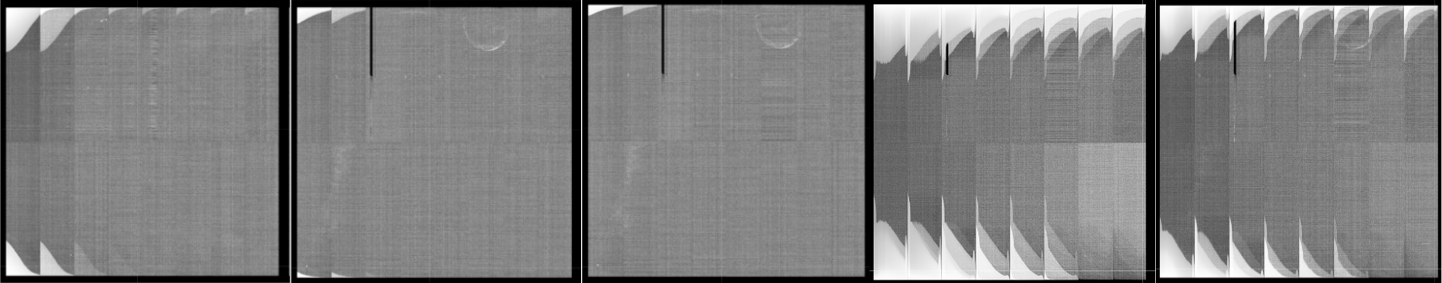
\includegraphics[width=0.9\textwidth]{sections/figures/Clear_R01_S10.png}
\end{centering}
\end{figure}

\emph{Figure showing the impact of the various types of clear on ITL
R01\_S10 after a saturated flat (bias after a saturated flat), from left
to right: 1 standard clear, 3 standard clears, 5 standard clears, 1 NoP
clear, 1 NoPSF clear}

One ITL sensor, R01\_S10,
presents a specific behavior that is not understood:

\begin{itemize}
\tightlist
\item
  It has a quite low full well (2/3 of nominal).
\item
  The 3 CCDs of this REB (REB1) have a gain 20\% lower than all other ITL CCDs.
\item
  The images taken after a large saturation, as seen in Figure
  \texttt{clear\ in\ itl\ R01\_S10\ \textless{}fig-image-itlR01\_S10clear\textgreater{}},
  show a large amount of uncleared charged (with the standard clear: 4
  amplifiers retain \textasciitilde500 rows of saturated signal!)
\end{itemize}

It appears that putting S3 low during the clear as done in NoP and NoPSF,
is even worse than a standard clear. This is strange, as a full frame
read, which does this too, manages to clear a saturated image. We can notice
that NoPSF is \textasciitilde50\% better than NoP, but still worse than
the standard clear, in particular for the 12 amplifiers that are almost correct
with the standard clear.

At this time we do not have a correct way to clear this
sensor once it collects a saturated flat, but it is not
known if a saturated star in this sensor, leaving signal in the
parallel overscan, will present the same clear issue.

\subsubsection{Conclusion}\label{conclusion}


{\small
\begin{longtable}{|p{0.17\linewidth}|p{0.17\linewidth}|p{0.17\linewidth}|p{0.17\linewidth}|p{0.17\linewidth}|p{0.17\linewidth}|}
\caption{\emph{This table summarizes the different clear methods used so far.}} \\
\hline
\textbf{Clear Type} & \textbf{Clear Duration} & \textbf{e2v after Saturated Flat} & \textbf{ITL after Saturated Flat} & \textbf{R01\_S10 ITL ``unique"} \\
\hline
\endfirsthead

%\hline
%\textbf{Clear Type} & \textbf{Clear duration} & \textbf{``E2V" after saturated Flat} & \textbf{``ITL`` after saturated Flat} & \textbf{R01 ITL ``unique"} \\
%\hline
\endhead

\hline
\endfoot

\hline
\endlastfoot

\textbf{Default Clear} 1 clear (seq. V29) & 65.5 ms & 1st row saturated signal up to row 50 & 1st row saturated signal up to 2nd row & first 500 rows saturated for 4 amp, 13 amp with signals \\
\textbf{Multi Clear} 3 clears (seq. V29) & 196.5 ms & No residual electrons & No residual electrons & first 150 rows saturated for 2 amp, 5 amp with signals \\
\textbf{Multi Clear} 5 clears (seq. V29) & 327.4 ms & No residual electrons & No residual electrons & first 100 rows saturated for 2 amp, 2 amp impacted \\
\textbf{Deep Clear} 1 clear (Seq. V23 DC) & 64.69 ms & 1st row saturated signal up to row <20 & tiny signal left in the first row & not measured \\
\textbf{No Pocket (NoP)} 1 clear (seq. V29) & 65.8 ms & signal up to row 20 & No residual electrons & first 1000 rows saturated for 16 amp, 16 amp with signals \\
\textbf{No Pocket Serial Flush (NoPSF)} 1 clear (seq. V29, V30) & 67.0 ms & No residual electrons & No residual electrons & first 750 rows saturated for 16 amp, 16 amp with signals \\
\end{longtable}
}


%\begin{longtable}{|p{0.18\linewidth}|p{0.13\linewidth}|p{0.13\linewidth}|p{0.13\linewidth}|p{0.13\linewidth}|p{0.13\linewidth}|p{0.16\linewidth}|}
%\caption{\emph{This table summarizes the different clear methods used so far.}} \\
%\hline
%\textbf{} & \textbf{Default Clear 1 Clear (seq. V29)} & \textbf{Multi Clear 3 Clears (seq. V29)} & \textbf{Multi Clear 5 Clears (seq. V29)} & \textbf{Deep Clear 1 Clear (Seq. V23 DC)} & \textbf{No Pocket (NoP) 1 Clear (seq. V29)} & \textbf{No Pocket Serial Flush (NoPSF) 1 Clear (seq. V29, V30)} \\
%\hline
%\endfirsthead
%
%\hline
%\textbf{} & \textbf{Default Clear 1 Clear (seq. V29)} & \textbf{Multi Clear 3 Clears (seq. V29)} & \textbf{Multi Clear 5 Clears (seq. V29)} & \textbf{Deep Clear 1 Clear (Seq. V23 DC)} & \textbf{No Pocket (NoP) 1 Clear (seq. V29)} & \textbf{No Pocket Serial Flush (NoPSF) 1 Clear (seq. V29, V30)} \\
%\hline
%\endhead
%
%\hline
%\endfoot
%
%\hline
%\endlastfoot
%
%Clear duration & 65.5 ms & 196.5 ms & 327.4 ms & 64.69 ms & 65.8 ms & 67 ms \\
%"E2V" after saturated Flat & 1st line saturated signal up to line 50 & No residual electrons & No residual electrons & 1st line saturated signal up to line <20 & signal up to line 20 & No residual electrons \\
%"ITL" after saturated Flat & 1st line saturated signal up to 2nd line & No residual electrons & No residual electrons & tiny signal left in the first line & No residual electrons & No residual electrons \\
%R01 ITL "unique" & first 500 lines saturated for 4 amp, 13 amp with signals & first 150 lines saturated for 2 amp, 5 amp with signals & first 100 lines saturated for 2 amp, 2 amp impacted & not measured & first 1000 lines saturated for 16 amp, 16 amp with signals & first 750 lines saturated for 16 amp, 16 amp with signals \\
%\end{longtable}


Even if NoP or NoPSF overcome the clear issue we had with ITL
sensors, the exception of R01\_S10 prevented
the usage of those sequencers for ITL devices for Run 7. Note that
aside from R01\_S10 the numbers of lines potentially
``not cleared" in ITL devices after saturated images are small (2 first rows), and they
correspond to a CCD area that is difficult to use anyway (sensor edges with low
efficiency). So at this stage the default clear is still our default
for ITL, and further studies to overcome the problem with
R01\_S10 are forseen (e.g., investigate using a continuous
serial flush during exposure at low rate, 10$^6$ pixel flushes in 15\,s).

\begin{quote}
For the other CCD type, after the studies in Run 7, we now have a good way
to fully clear the e2v devices through the NopSF clear. The NoPSF clear
grants that the first 50 rows of e2v CCDs that had un-cleared
electrons from the previous exposure are now free of such
contamination.
\end{quote}

For the time being:

\begin{itemize}
\tightlist
\item
  For e2v, NoPSF will be the default clear method.
\item
  For ITL, the original clear (serial phase 3 always), slightly extended
  in time to match the NoPSF e2v clear execution time, will stay the
  default method.
\end{itemize}

\subsection{Toggling the RG Bit During Parallel Transfer}\label{noRGe2v}
This investigation comes from an analogy drawn with the ITL sequencer file. Although the vendor recommended toggling the RG bit at the end of the parallel transfer, it was unclear whether this step was truly necessary. Given the improvements observed in ITL devices, applying this approach to e2v devices also became an area of interest.

\subsection{Disable IDLE FLUSH}\label{thermal-optimization}

IDLE\_FLUSH is one of the main settings in the sequencer file that enables the sequencer output to run while in the IDLE state (the period between one exposure and the next). The specific implementation of IDLE\_FLUSH can be selected from various functions in the sequencer file. In Run 5, we chose the \texttt{ReadPixel} function, which reads out a pixel. This choice was initially made to mitigate the so-called yellow corner issue, a 2D structure of elevated signal near an amplifier corner observed in bias and dark exposures for certain amplifiers on e2v CCDs (see details in \hyperref[U2024]{{[}U2024{]}}).

However, it was reported that running IDLE\_FLUSH exacerbates the Divisidero tearing issue. Divisidero tearing appears as a signal deficiency at amplifier boundaries in e2v sensors, accompanied by increased signal in adjacent columns. Additionally, using \texttt{ReadPixel} as the IDLE\_FLUSH function has the highest thermal impact because it continuously operates the Analog-to-Digital Converter at its maximum rate. This results in a significant difference in power consumption, more than 50\,W over all rafts, between the exposure state and the IDLE state. Consequently, the focal plane experiences a temperature variation of approximately 2 deg C between periods of image acquisition and idle periods (Figure~\ref{IdleFlushEffect}).

\begin{figure}
\begin{centering}
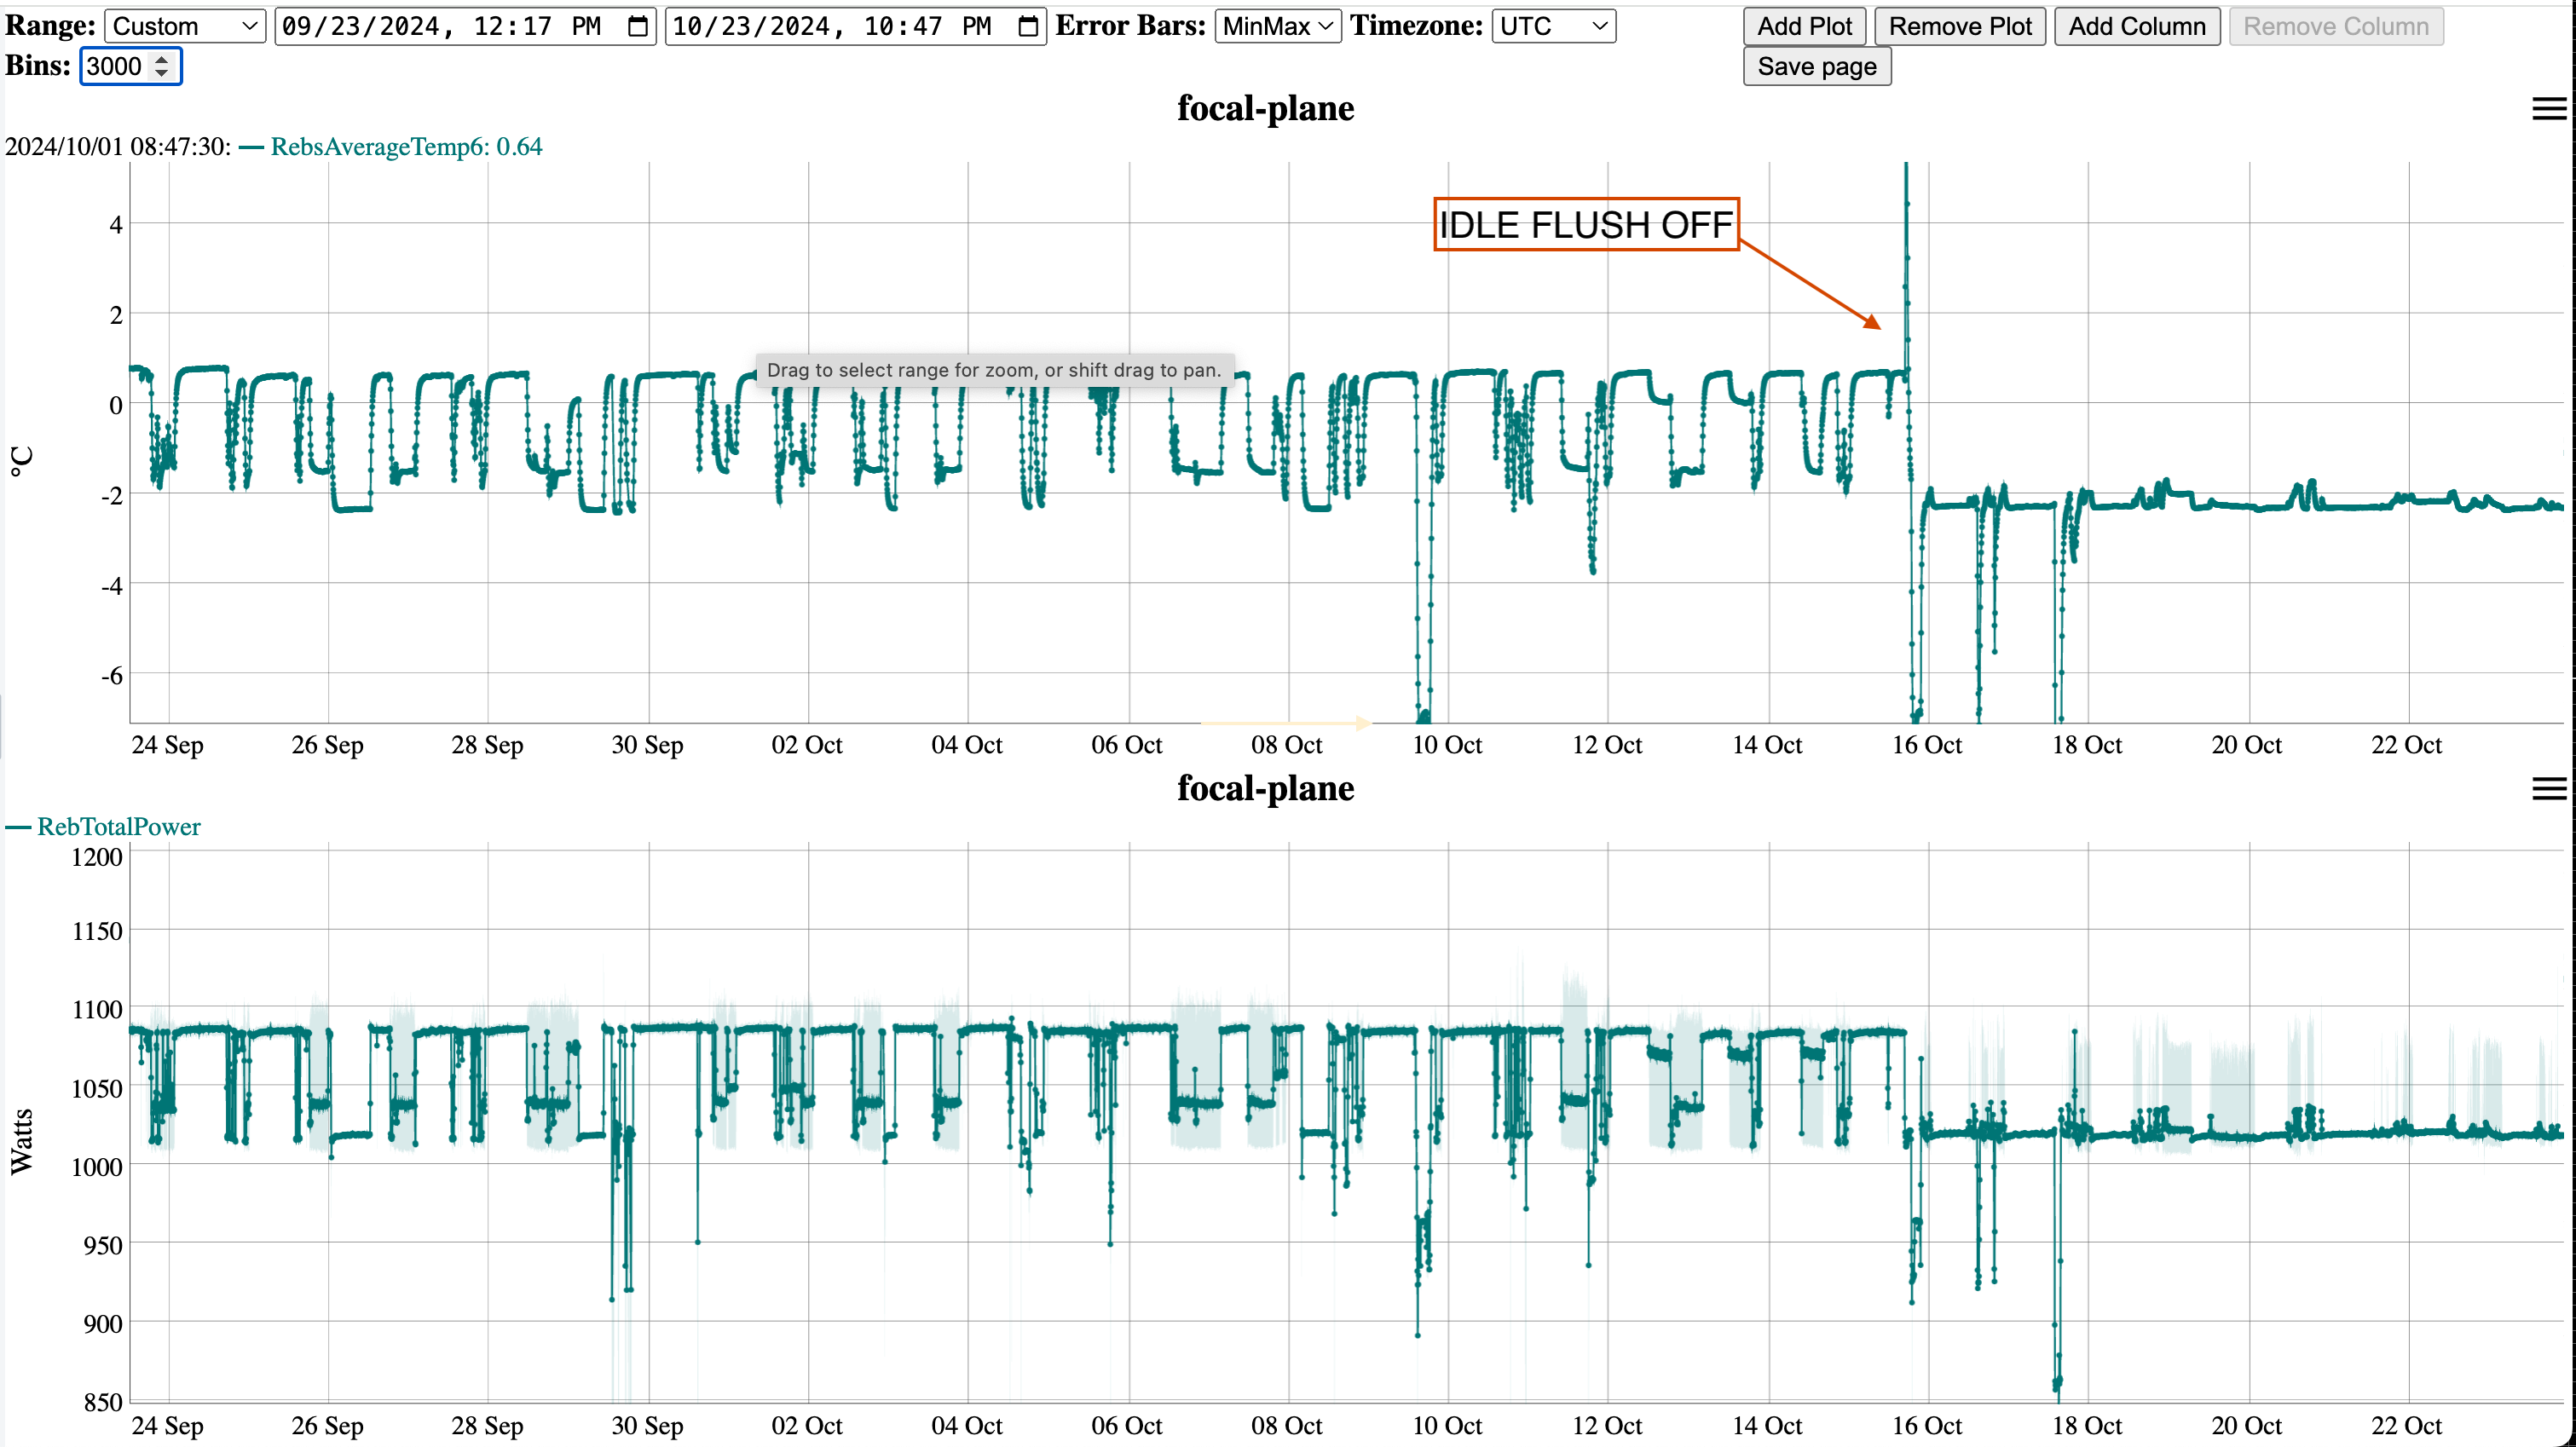
\includegraphics[width=0.9\textwidth]{sections/figures/REB_power_temp6_sept24_to_Oct23.png}
\end{centering}
\caption{Impact of enabling and disabling IDLE\_FLUSH on focal-plane temperature and power consumption.}\label{IdleFlushEffect}
\end{figure}

This temperature variation in the focal plane can lead to changes in the REB temperature, potentially causing gain variations or instability in the bias. Based on these considerations, we decided to disable IDLE\_FLUSH. The impact of this change on bias stability is discussed in Sections~\ref{bias-stability-2} and~\ref{gain-stability-2}.

\begin{figure}
\begin{centering}
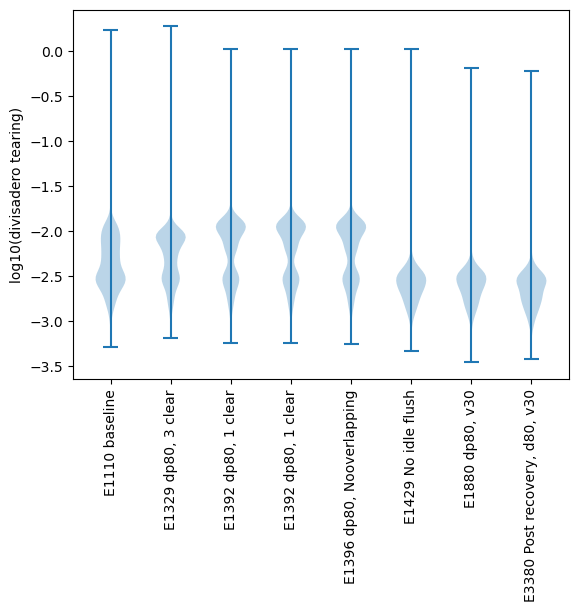
\includegraphics[width=0.9\textwidth]{sections/figures/divisadero.png}
\end{centering}
\caption{Impact of disabling IDLE\_FLUSH on Divisadero tearing}\label{IdleFlushEffect:divisadero}
\end{figure}
Figure \ref{IdleFlushEffect:divisadero} shows the impact on the Divisadero tearing. The runs shown here are selected B protocol runs with different settings in the time order. There were a couple of changes: 1) switching to narrower parallel swing voltage, 2) changing the number of clears before the exposure, 3) disabling IDLE\_FLUSH.  Some minor changes in each changes are also included such as changing the number of clears, or changing the sequencer file (the change from v29 to v30  is primarily incorporation of the change in the clear). The figure includes both ITL and e2v results. The two distinct distributions in earlier runs correspond to the differences between the two types of CCD (the higher one is e2v and the lower one is ITL). The greatest change can be seen when we switched to not running IDLE\_FLUSH at E1429, which brought the overall distribution down. The two distributions became indistinguishable, which indicates the majority of the Divisadero tearing for e2v is mitigated.

E3380 was the run taken after the recovery from the shutdown due to poor performance of the Pumped Coolant System. This fact confirms that the metric is consistent over power cycling of LSSTCam.

\subsection{Summary}\label{summary}
e2v sensors had persistence. We confirmed that narrowing the parallel swing voltage of the e2v CCD operation greatly reduced persistence. As penalties, we observed a full well reduction of 22\% and a \textasciitilde10\% increase of the
brighter-fatter effect, essentially in an isotropic way.

We developed v30 sequencer files that have guider functionality built in and an improved clear of No Pocket Serial Flush.

We also disabled IDLE\_FLUSH to improve the thermal situation and the Divisadero tearing.

Sequencer files have undergone evolution for both ITL and e2v versions.
The final sequencer file from Run 6 was the
v26noRG version for ITL and the regular v26
for e2v. The suffix noRG indicates that the
RG bit is not toggled during parallel transfer. This modification
appears to enhance the stability of the bias structure for most ITL
amplifiers.

During Run 7, several changes were implemented, as described below:

\begin{itemize}
\tightlist
\item
  v27 incorporated guider functionalities, including ParallelFlushG and
  ReadGFrame. However, the noRG change was inadvertently included.
  Consequently, we abandoned this version and switched to v28.
\item
  v28 sequencer files merged v26noRG and
  v27. \url{https://rubinobs.atlassian.net/browse/LSSTCAM-5}
\item
  v29 introduced changes to speed up the guider.
  \url{https://rubinobs.atlassian.net/browse/LSSTCAM-34}
\item
  v30 primarily focused on e2v. We introduced a new approach to NopSf
  for e2v CCDs
  \url{https://github.com/lsst-camera-dh/sequencer-files/pull/17}. To
  align timing with the ITL version, a change was made.
  \url{https://github.com/lsst-camera-dh/sequencer-files/pull/18}
\end{itemize}


\section{Characterization \& Camera
stability}\label{characterization-camera-stability}

\subsection{Final characterization background}\label{background}

\begin{longtable}[H]{@{}
  >{\raggedright\arraybackslash}p{(\linewidth - 4\tabcolsep) * \real{0.1806}}
  >{\raggedright\arraybackslash}p{(\linewidth - 4\tabcolsep) * \real{0.2083}}
  >{\raggedright\arraybackslash}p{(\linewidth - 4\tabcolsep) * \real{0.2639}}@{}}
\toprule\noalign{}
\label{runTable}
\begin{minipage}[b]{\linewidth}\raggedright
\begin{quote}
Run Type
\end{quote}
\end{minipage} & \begin{minipage}[b]{\linewidth}\raggedright
Cerro Pachón Initial Run
\end{minipage} & \begin{minipage}[b]{\linewidth}\raggedright
Cerro Pachón Final Run
\end{minipage} \\
\midrule\noalign{}
\endhead
\bottomrule\noalign{}
\endlastfoot
B Protocol & \begin{minipage}[t]{\linewidth}\raggedright
\begin{quote}
E1071
\end{quote}
\end{minipage} & \begin{minipage}[t]{\linewidth}\raggedright
\begin{quote}
E
\end{quote}
\end{minipage} \\
\begin{minipage}[t]{\linewidth}\raggedright
\begin{quote}
PTC
\end{quote}
\end{minipage} & \begin{minipage}[t]{\linewidth}\raggedright
\begin{quote}
E749
\end{quote}
\end{minipage} & \begin{minipage}[t]{\linewidth}\raggedright
\begin{quote}
E
\end{quote}
\end{minipage} \\
\caption{Reference runs for Run 6 and Run 7 comparisons}
\end{longtable}

\subsubsection{Stability flat metrics}\label{stability-flat-metrics}


\paragraph{Serial CTI}\label{serial-cti}




\paragraph{Parallel CTI}\label{parallel-cti}




\subsubsection{Dark metrics}\label{dark-metrics}

\paragraph{Dark current}\label{dark-current}




\paragraph{Bright defects}\label{bright-defects}

\subsubsection{Flat pair metrics}

\paragraph{Linearity and PTC turnoff}\label{linearity-and-ptc-turnoff}



\paragraph{PTC Gain}\label{ptc-gain}




\paragraph{\texorpdfstring{Brighter fatter a{00}
coefficient}{Brighter fatter a00 coefficient}}\label{brighter-fatter-a00-coefficient}



\paragraph{Brighter-Fatter Correlation}\label{brighter-fatter-correlation}



\paragraph{Row-means variance}\label{row-means-var}



\paragraph{Divisadero Tearing}\label{divisadero-tearing}



\paragraph{Dark defects}\label{dark-defects}



\subsubsection{Persistence}\label{persistence}



\subsubsection{Differences between run 7 initial and run 7 final measurements}\label{differences-from-previous-runs}

% Add something about the major differences between the runs

% Please add the following required packages to your document preamble:
% \usepackage{multirow}
\begin{table}[H]
\begin{tabular}{|l|ll|ll|}
\hline
\multirow{2}{*}{Parameter [unit]}          & \multicolumn{2}{l|}{E2V}                   & \multicolumn{2}{l|}{ITL}                    \\ \cline{2-5} 
                                    & \multicolumn{1}{l|}{Run 7 initial}     & Run 7 final     & \multicolumn{1}{l|}{Run 7 initial}     & Run 7 final      \\ \hline
Serial CTI {[}\%{]}                 & \multicolumn{1}{l|}{} &  & \multicolumn{1}{l|}{} &  \\ \hline
Parallel CTI {[}\%{]}               & \multicolumn{1}{l|}{} &  & \multicolumn{1}{l|}{} &  \\ \hline
Dark current {[}e-/pix/s{]}         & \multicolumn{1}{l|}{}          &           & \multicolumn{1}{l|}{}          &            \\ \hline
Bright defects {[}count{]}          & \multicolumn{1}{l|}{}          &           & \multicolumn{1}{l|}{}          &            \\ \hline
Linearity turnoff {[}e-{]}          & \multicolumn{1}{l|}{} &  & \multicolumn{1}{l|}{} &   \\ \hline
PTC turnoff {[}e-{]}                & \multicolumn{1}{l|}{}  &   & \multicolumn{1}{l|}{}  &    \\ \hline
PTC Gain {[}e- / ADU{]}             & \multicolumn{1}{l|}{}    &    & \multicolumn{1}{l|}{}    &      \\ \hline
PTC $a_{00}$ [$\frac{1}{pix^2}$]      & \multicolumn{1}{l|}{} &  & \multicolumn{1}{l|}{} &   \\ \hline
BF x-correlation                    & \multicolumn{1}{l|}{}    &  & \multicolumn{1}{l|}{}    &      \\ \hline
BF y-correlation                    & \multicolumn{1}{l|}{}    &  & \multicolumn{1}{l|}{}    &      \\ \hline
Row-means variance                  & \multicolumn{1}{l|}{}    &  & \multicolumn{1}{l|}{}    &      \\ \hline
Dark defects {[}count{]}            & \multicolumn{1}{l|}{}          &           & \multicolumn{1}{l|}{}          &            \\ \hline
Divisadero tearing maximum {[}\%{]} & \multicolumn{1}{l|}{}          &           & \multicolumn{1}{l|}{}          &            \\ \hline
Persistence {[}ADU{]}               & \multicolumn{1}{l|}{}          &           & \multicolumn{1}{l|}{}          &            \\ \hline
\end{tabular}
\end{table}


\subsection{Changes in the dead amplifiers}\label{deadamplifiers}

\subsection{Full well measurements}\label{fullwell}

\subsection{Non-linearity studies}\label{nonlinearity}
PTC runs are meant primarily to measure variance and co-variance curves. We collect pairs of flat images, from an integrating sphere fed by various LEDs, that  illuminates the focal plane. To cover the entire dynamic range of the CCDs, we vary the length of the LED flash, the number of flashes, and the current of the LED. These data sets can be used to measure nonlinearity by comparing the CCD response to the integrated signal measured from a photodiode installed on a port of the integrating sphere that feeds a picoammeter. To avoid any shortcomings from picoammeter nonlinearity, we only compare photodiode signals of the same amplitude (illumination intensity) but different durations. We do not assume that integrated charges measured at different LED currents (and hence different photodiode currents) are on the same scale, although this turns out to be essentially true, as discussed later. 

For the nonlinearity study, we use the average signal measured on each CCD channel separately, using 2D overscan subtraction and masking outlier pixels. The photodiode signal is simply bias-subtracted and time-integrated. 

Technically, we model the nonlinearity using a spline function that we fit to the CCD/photodiode data pairs by minimizing:
\begin{equation}
Q = \sum_{ij} w_{ij}^2 \left( \frac{ S(\mu_{ij}) +\mu_{ij}  }{D_{ij} f_i} -1 \right)^2
\label{eq:nonlin0}
\end{equation}
where $Q_{ij}$ is the CCD signal measured in exposure $j$ at LED current $i$,
$D_{ij}$ is the corresponding photodiode signal, $f_i$ is the ``photodiode factor" for current $i$, $S$ is the spline nonlinearity correction, and $w_{ij}$ is some weight. We add two constraints: the average of the spline over the fitting range is zero $<S(\mu)=0>$, and $S(0) = 0$. We carry out this fit for all video channels separately. The weights $w_{ij}$ are modeled using an expression determined empirically, $w_{ij} = 1/\sqrt(c^2+v^2/m_{ij})$, and the two extra parameters, $c$ and $v$ are also fitted by modifying the expression \ref{eq:nonlin0}:
\begin{equation}
Q = \sum_{ij} w_{ij}^2 \left( \frac{ S(\mu_{ij}) +\mu_{ij}  }{D_{ij} f_i} -1 \right)^2 - 2 \Sigma_{ij} \log w_{ij}
\label{eq:nonlin1}
\end{equation}
We fit the spline coefficients, the $f_i$ factors (there are typically 3 of them), and the weight parameters $c$ and $v$. We perform an iterative 5$\sigma$ outlier rejection which rejects on average $\sim $0.5 \% of the data points.  
We are firstly interested in the spline correction, and we give an example in Fig. \ref{fig:nonlin_model}.

\begin{figure}
\begin{centering}
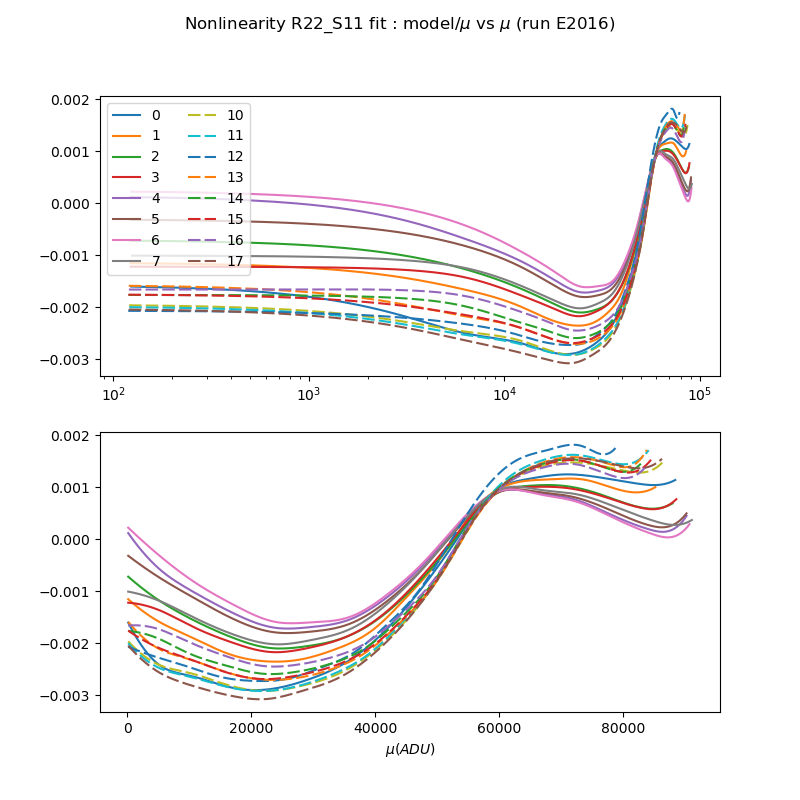
\includegraphics[width=0.9\textwidth]{sections/figures/E2016_nonlin_model.png}
\end{centering}
\caption{Fitted non-linearity spline for the 16 channels of R22\_S11 (using the PTC run E2016). The distortion around 60000 ADUs is due to the preamplifier. The curves obtained for the same sensor from another data set are extremely similar. \label{fig:nonlin_model}}


\end{figure}



\subsection{Guider operation}\label{guider-operation}

This section describes guider operation.

\begin{itemize}
\tightlist
\item
  Initial guider operation
\item
  Power cycling the guiders to get to proper mode
\item
  Synchronization
\item
  Guider ROI characterization
\end{itemize}

\subsection{Defect stability}\label{defect-stability}

This section describes defect stability.

\begin{itemize}
\tightlist
\item
  Bright defects
\item
  Dark defects with picture frame
\end{itemize}

\subsection{Bias stability}\label{bias-stability-2}

We have found bias instabilities, typically above the 1 ADU level, for a number of CCDs in the focal plane, both ITL and e2v. Two main kinds of instability are observed:

\begin{enumerate}
\tightlist
\item
  ITL bias jumps : large variations of the column-wise structure from
  exposure to exposure.
\item
  e2v yellow corners : a residual 2D shape of the bias even after
  2D-overscan correction. These residuals depend on the acquisition
  sequence and the exposure time, and the enhancement is greatest near the readout nodes (hence `yelllow corner').
\end{enumerate}

Both issues were observed and deeply studied in Run 6 EO data. The ITL
issue is believed to be phase shifts in clocks between Readout
Electronics Boards (REBs) because REBs rely on the frequency converted
from their natural frequency. We tried to mitigate the e2v issue by
optimizing the acquisition configuration in Run 7.

For the baseline acquisition configuration (see conclusion), three
relevant stability runs were recorded:

\begin{enumerate}
\tightlist
\item
  Run E2136: 15\,s darks with some very long delays throughout the run
\item
  Run E2236: 50 15\,s darks, 50 biases recorded with 30\,s delays between
  exposures
\item
  Run E2330: 15\,s and 30\,s darks with variable delays between exposures
\end{enumerate}

To analyze these runs for bias instability, the eo\_pipe bias
stability task is used.  For the ISR part, a serial
%(\textquotesingle mean\phantomsection\label{per_row}{per\_row}\textquotesingle)
(`meanper\_row')
overscan correction and a bias subtraction (computed from the
corresponding B-protocol run) are applied. The final data product of the task is the
mean of the per-amplifier science image over the full set of exposures
of the run. Two typical examples from Run E2136 are shown in the figures
below. In the stable case, the variations are typically at the 0.1 ADU
level; in the unstable case, the variations range up to 4 ADUs.

\begin{figure}[h]
\centering
\begin{minipage}[b]{0.45\textwidth}
\centering
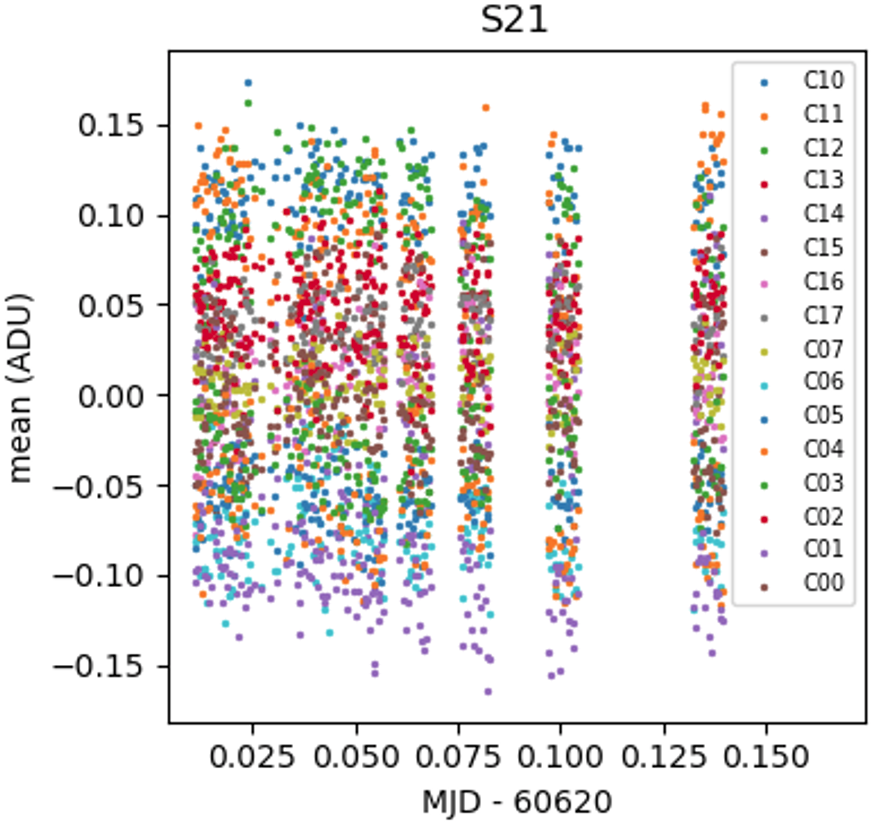
\includegraphics[width=\textwidth]{sections/figures/E2136_R21_S21.png}
\end{minipage}
\hfill
\begin{minipage}[b]{0.45\textwidth}
\centering
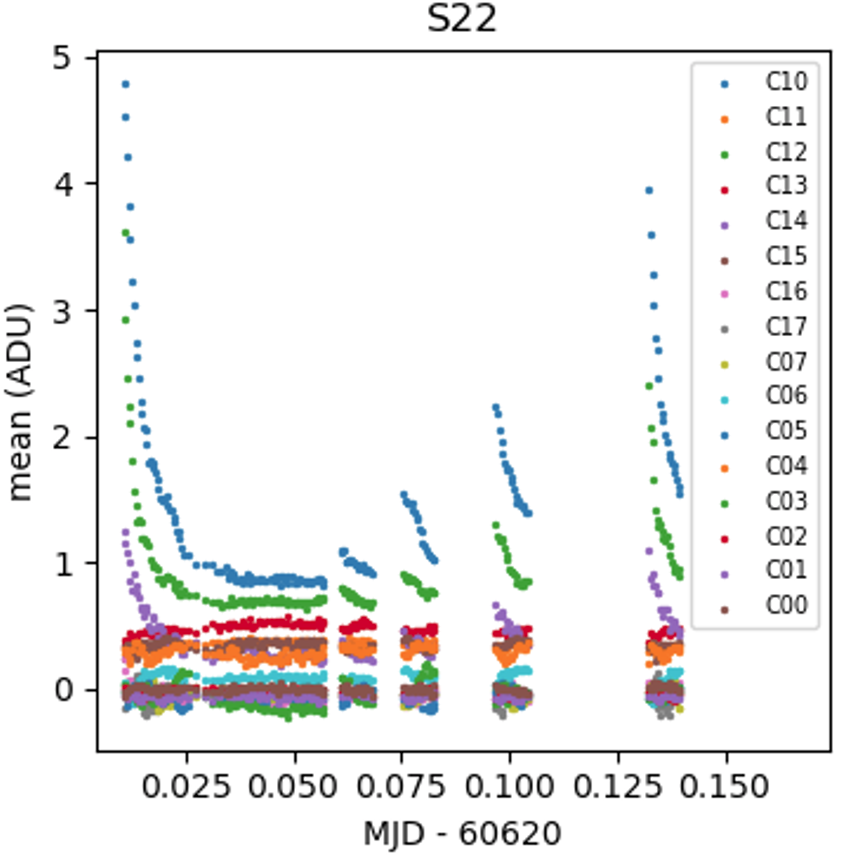
\includegraphics[width=\textwidth]{sections/figures/E2136_R23_S22.png}
\end{minipage}
\caption{(left) Stable case (R21\_S21); (right) Unstable case (R23\_S22)}
\end{figure}


A comparison of the results for an unstable CCD is shown below for the
three runs.

\begin{figure}[htbp]
\centering
\begin{minipage}[b]{0.45\textwidth}
    \centering
    \includegraphics[width=\textwidth]{sections/figures/E2136_R33_S02.png}
    \caption{Run E2136, R33\_S02}
\end{minipage}
\hspace{0.05\textwidth}
\begin{minipage}[b]{0.45\textwidth}
    \centering
    \includegraphics[width=\textwidth]{sections/figures/E2236_R33_S02.png}
    \caption{Run E2236, R33\_S02}
\end{minipage}

\vspace{0.05\textwidth}

\begin{minipage}[b]{0.45\textwidth}
    \centering
    \includegraphics[width=\textwidth]{sections/figures/E2330_R33_S02.png}
    \caption{Run E2330, R33\_S02}
\end{minipage}
\hspace{0.05\textwidth}
\hfill
\begin{minipage}[b]{0.45\textwidth}
    \centering
    % 空白セルとして保持
\end{minipage}
\end{figure}


%\begin{figure}
%\begin{centering}
%\includegraphics[width=0.9\textwidth]{sections/figures/E2136_R33_S02.png}
%\end{centering}
%\caption{Run E2136, R33 S02}
%\end{figure}
%
%\begin{figure}
%\begin{centering}
%\includegraphics[width=0.9\textwidth]{sections/figures/E2236_R33_S02.png}
%\end{centering}
%\caption{Run E2236, R33 S02}
%\end{figure}
%
%\begin{figure}
%\begin{centering}
%\includegraphics[width=0.9\textwidth]{sections/figures/E2330_R33_S02.png}
%\end{centering}
%\caption{Run E2330, R33 S02}
%\end{figure}

To highlight the 2D shape differences in ITL bias instability, a 2D-overscan correction
is applied. A few exposures illustrating the variations of the 2D shape
for an unstable CCD are shown below. The 2D shape of the image in
amplifier C01 is different in the 3 cases.

\begin{figure}[htbp]
\centering
\begin{minipage}{0.45\textwidth}
    \centering
    \includegraphics[width=\textwidth]{sections/figures/E1880_bias_R33_S02.png}
    \caption{Bias exposure, run 1880, R33\_S02}
\end{minipage}
\hfill
\begin{minipage}{0.45\textwidth}
    \centering
    \includegraphics[width=\textwidth]{sections/figures/E2136_dark15_R33_S02.png}
    \caption{15-s dark exposure, run E2136 in 'stable' conditions, R33\_S02}
\end{minipage}

\vspace{0.5cm}

\begin{minipage}{0.45\textwidth}
    \centering
    \includegraphics[width=\textwidth]{sections/figures/E2136_dark15_delay_R33_S02.png}
    \caption{15\,s dark exposure, run E2136 after a 3\,min delay, R33\_S02}
\end{minipage}
\hfill
\begin{minipage}{0.45\textwidth}
    \centering
\end{minipage}
\end{figure}

%\begin{figure}
%\begin{centering}
%\includegraphics[width=0.9\textwidth]{sections/figures/E1880_bias_R33_S02.png}
%\end{centering}
%\caption{Bias exposure, run 1880, R33 S02}
%\end{figure}
%
%\begin{figure}
%\begin{centering}
%\includegraphics[width=0.9\textwidth]{sections/figures/E2136_dark15_R33_S02.png}
%\end{centering}
%\caption{15-s dark exposure, run E2136 in
%\textquotesingle stable\textquotesingle{} conditions, R33 S02}
%\end{figure}
%
%\begin{figure}
%\begin{centering}
%\includegraphics[width=0.9\textwidth]{sections/figures/E2136_dark15_delay_R33_S02.png}
%\end{centering}
%\caption{15-s dark exposure, run E2136 after a 3-minute delay, R33 S02}
%\end{figure}

In order to quantify the number of unstable e2v amplifiers, a stability
metric \emph{d} is defined from the eo\_pipe
stability task data products. More precisely, \emph{d} is defined, for a
given amplifier in a given run, as the difference between the 5th and
95th percentiles of the image mean over all the bias image acquisitions. The
distribution of \emph{d} for run E2136 is shown below. Applying a
threshold at 0.3\,ADU, 51 amplifiers are identified as unstable (see the
corresponding mosaic). This corresponds to \textasciitilde3\% of the e2v
amplifiers.

\begin{figure}[htbp]
\centering
\begin{minipage}{0.45\textwidth}
    \centering
    \includegraphics[width=\textwidth]{sections/figures/E2136_distribution_d.png}
    \caption{Distribution of the stability metric for the e2v amplifiers in run E2136}
\end{minipage}
\hfill
\begin{minipage}{0.45\textwidth}
    \centering
    \includegraphics[width=\textwidth]{sections/figures/E2136_mosaic_d.png}
    \caption{Mosaic of e2v amplifiers identified as unstable (white color) in run E2136}
\end{minipage}
\end{figure}

%\begin{figure}
%\begin{centering}
%\includegraphics[width=0.9\textwidth]{sections/figures/E2136_distribution_d.png}
%\end{centering}
%\caption{Distribution of the stability metric for the e2v amplifiers in
%run E2136}
%\end{figure}
%
%\begin{figure}
%\begin{centering}
%\includegraphics[width=0.9\textwidth]{sections/figures/E2136_mosaic_d.png}
%\end{centering}
%\caption{Mosaic of e2v amplifiers identified as instable (white color)
%in run E2136}
%\end{figure}

Further studies are required in order to converge on the best mitigation
strategy for the start of the LSST survey.

\subsection{Gain stability}\label{gain-stability-2}
The ``relative gain" is defined as the ratio of the signal observed in a CCD image segment divided by the integration of the photodiode current with respect to an arbitrary normalization.
With a fixed flat illumination, the variation of the relative gain over successive exposures can be utilized to investigate the gain stability. We acquired flat images at the same flux level with two distinct temperature conditions: either intentionally altered or maintained constant.
\begin{itemize}
    \item E1496 (dp80, constant temp, v29\_Nop, nm750, 10k e-)
    \item E1367 (dp80, temp swing, v29, nm750, 50k e-)
    \item E756 (dp80, gain stability @ 50k e-)
    \item E1362 (dp80, 10k e-)
\end{itemize}
(YU: WORK IN PROGRESS)


\begin{figure}[htbp]
\centering
\begin{minipage}{0.45\textwidth}
    \centering
    \includegraphics[width=\textwidth]{sections/figures/RelgainParametersTrending.png}
    \caption{Distribution of the stability metric for the e2v amplifiers in run E2136}
\end{minipage}
\hfill
\begin{minipage}{0.45\textwidth}
    \centering
    \includegraphics[width=\textwidth]{sections/figures/RelgainDetail.png}
    \caption{Mosaic of e2v amplifiers identified as unstable (white color) in run E2136}
\end{minipage}
\end{figure}


\section{Sensor features}\label{sensor-features}

\subsection{Tree rings}\label{tree-rings}
\subsubsection{Center of the Tree Ring}
So far we have been using the four average position for the center of the Tree ring, according to the pattern direction, however now we have new data with 0 V of back bias voltage, we wanted to make sure if the error in center of the ring position is small enough and if we need to use individual center position for each sensor. 

This is the position of Tree ring center measured for the 189 sensors. We decided to use center of each sensor instead of the average value. 

\begin{figure}
\begin{centering}
\includegraphics[width=0.9\textwidth]{sections/figures/TR_centers.png}
\end{centering}
\caption{The center of the Tree Rings were measured for all 189 LSST sensors. Red point indicates the average center on each direction.}
\end{figure}

\subsubsection{Radial study}
Radial study for Tree rings pattern has been done to see if the rings are perfectly circular in shape. 

This is the image of transforming the flat image into the radial image as the y axis to be the distance from the center of the rings. 

\begin{figure}
\begin{centering}
\includegraphics[width=0.9\textwidth]{sections/figures/TR_subtraction.png}
\end{centering}
\caption{Folding image on diagonal line from the center of the ring, and subtracting from each other.}
\end{figure}

\begin{figure}
\begin{centering}
\includegraphics[width=0.9\textwidth]{sections/figures/TR_radial.png}
\end{centering}
\caption{Radial study of the Tree Rings. Right: image subtracting left to right, right to left.}
\end{figure}

\subsubsection{Effect of diffuser}
We expect that with the diffuser installed, there will be less contribution from effects such as CMB and weather patterns discussed in \S~XX. Comparing R22\_S12 of Run 6 run 13379 (without diffuser) with Run 7 E937 (with diffuser), we could check significant improvement from the diffuser.
\paragraph{Tree rings without diffuser}

\begin{figure}
\begin{centering}
\includegraphics[width=0.9\textwidth]{sections/figures/TR_wo_diffuser.png}
\end{centering}
\caption{Tree ring without diffuser}
\end{figure}

\paragraph{Tree rings with diffuser}

\begin{figure}
\begin{centering}
\includegraphics[width=0.9\textwidth]{sections/figures/TR_w_diffuser.png}
\end{centering}
\caption{Tree ring with diffuser}
\end{figure}


\subsubsection{Voltage dependency}
\subsubsection{Wavelength dependency}


\subsection{ITL Dips}\label{itl-dips}

One of the phenomena that was studied in the later part of Run 7 was so-called 
`ITL dips'. These were discovered in LSST ComCam on-sky data as
bleed trails from bright stars that traversed the entire detector,
crossing the amplifier boundaries. These bleed trails are unique
though in that the core of the bleed trail is actually `dark'
compared to the wings of the trail, with a flux $\sim$2\% less relative to the rest of the
bleed trail.

We investigated whether ITL dips could also be observed in the CCDs of
LSSTCam. For this study, we used spots and rectangles projected onto the focal plane by the 4K
projector. The spots were approximately 30 pixels across
and were projected onto every amplifier segment of each detector. The rectangles were only
in the top right amplifier (C10). One consideration with this spot
projection was that the projector also provided background illumination. This led to the spots having a peak signal only 6 times greater
than the background and the rectangles having a peak signal 30 times greater
than the background.

We were unable to find any evidence of ITL
dips in the images. Below are the images themselves along with binned horizontal
cutouts of the the amplifier below the source. These show the background
pattern of the projector, but no 2\% dip.

While we were not able to find evidence of the ITL dip in Run 7 data, it
is still not clear whether the effect will be visible in LSSTCam on-sky data.
The photon rate of the in-lab data was roughly XXX per second for the 15\,s exposures. The stars that were seen in ComCam with the ITL dip
have a magnitude of XXX corresponding to a photon rate of XXX. This is
combined with a sky background of XXX as compared with the lab sensor
background of XXX.

\subsection{Vampire pixels}\label{vampire-pixels}

\subsubsection{First observations}\label{first-observations}

Vampire pixels were first observed in ComCam observations {[}need more
info to properly give context{]} - Andy's study on Oct.
8 - Agnes masking effort

\subsubsection{LSSTCam vampire pixel
features}\label{lsstcam-vampire-pixel-features}

The vampire pixels have distinct features, both on the individual defect
level, and across the focal plane

\paragraph{Individual vampire
features}\label{individual-vampire-features}

\begin{itemize}
\tightlist
\item
  General size
\item
  Radial kernel
\item
  uniformity
\end{itemize}

\paragraph{Vampire features across the focal
plane}\label{vampire-features-across-the-focal-plane}

\begin{itemize}
\tightlist
\item
  sensor type
\item
  static or dynamic
\item
  higher concentrations? Particularly bad sensors?
\end{itemize}

\subsubsection{Current masking
conditions}\label{current-masking-conditions}

\begin{itemize}
\tightlist
\item
  Bright pixels
\item
  Dark pixels
\item
  Jim's task
\end{itemize}

\subsubsection{Analysis of flats}\label{analysis-of-flats}

\begin{itemize}
\tightlist
\item
  LED effect
\item
  Intensity effect
\end{itemize}

\subsubsection{Analysis of darks}\label{analysis-of-darks}

\begin{itemize}
\tightlist
\item
  Previous LED effect
\item
  Intensity of LED effect
\item
  dark cadence and exposure times
\end{itemize}

\subsubsection{Current models of
vampires}\label{current-models-of-vampires}

\begin{itemize}
\tightlist
\item
  Tony \& Craig model
\item
  Others?
\end{itemize}



\subsection{Phosphorescence}\label{phosphorescence}

The Run 7 persistence optimization process (cf. \S\ref{persistence-optimization-1}) used a short EO image acquisition sequence and analysis script, which rapidly provided persistence performance metrics as feedback for each configuration tested. Thus, as soon as the e2v sensors were shown to be nearly free of {\it their} undesirable effects by reducing their clock swing voltages from 9.3\,V down to 8.0\,V, a similar persistence (or memory effect) was immediately noticed, affecting a subset of the ITL sensors. This discovery gained immediate interest for at least two reasons: (1) that it had not been detected in prior EO campaigns, and (2) that the new memory effect on certain ITL sensors was morphologically distinct from what had just been cured on the e2vs. 

The ITL sensors with the largest memory effect were evaluated, and the following observations were made:
\begin{itemize}
    \item[1.] The morphology of the expressed memory effect in the first dark image acquired after the trigger (the saturation flat) was reminiscent of the {\it ``coffee stains''} seen on the same sensors in flat field response, but with the opposite polarity. The ``coffee stains'' are commonly assumed to be associated with minor, localized variations in the sensors' antireflective coatings or perhaps a very thin, dead layer associated with the backside surface: they tend to be larger in amplitude when shorter wavelengths are used to expose the sensors with flat field illumination.
    \item[2.] The attenuation timescale of the memory effect is curiously comparable to the timescales that were seen in the persistence suffered by the e2v sensors (which are believed due to exposure of surface states by the collected conversions, on the semiconductor-insulator interface on the front side): exponential time constants of between 20 and 40\,s, which unfortunately are in turn very close to the nominal exposure cadence for the LSST survey.
    \item[3.] The similarity in memory effect time constants (de-trapping charges from surface states near the channel on the front side -- the e2v case -- vs. either de-trapping of charges located near the backside window surface or relaxation by photon emission by some excited states there -- the ITL case) can be thought to favor the electron de-trapping mechanism, just from the other surface. Otherwise, the nearly matched time constants would have to be seen as an improbable coincidence.
    \item[4.] A list of 12 ITL sensor serial numbers corresponding to those showing the memory effect was communicated to Mike Lesser at ITL. The list of parts shared certain properties according to his notes, and led him to develop a placeholder theory that would partially explain the mechanism. If true, it could explain what might be responsible for both the coffee stains and the memory effect with similar spatial distribution. He wrote that he tried, but was unsuccessful in diagnosing, using optical characterization tools (e.g., ellipsometer), any changes in optical constants on the affected regions of the ``stained'' sensors. The origin of the ``stains'', according to this theory, is as a consequence of there being ``raised spots'' on the sensors' backside surfaces that survive the final silicon acid etch. The raised silicon areas could potentially be trapping the resist used during the cleaning process that directly follows the etching step. Lesser wrote that the resist is wax-based and {\it does} fluoresce. If the theory is correct, he suggests that the medium would definitely be located {\it under} the AR coating and related neither to the coating nor the oxidation processes.
    \item[5.] Discussions among the Rubin team led to the following distinction of terminology that served to name the ITL memory effect in question. The main difference between ``fluorescence'' and ``phosphorescence'' is in that the former is considered prompt re-emission and the later could be re-emission following a finite characteristic time constant. Characteristic time constants are in the nanosecond scale for fluorescence, while for phosphorescence it would be in the milliseconds to seconds range. For the purpose of this discussion, we adopt the word ``phosphorescence'' to refer to the memory effect present in some ITL sensors.
    \item[6.] Lesser mentioned that the wax-based resist fluoresces (that would be the prompt mechanism with very short relaxation time). If there is any such residual material between the coating and the passivated silicon, it would be natural to expect a halo that would accompany any sharp (PSF-scale features) illumination that passes through these ``stains'' on the sensor surface: a scatter term with low integrated amplitude, whose scale should depend upon the re-emission wavelength. This has not yet been seen in lab data but may appear once the Camera goes on-sky.
    
% I highly doubt that they are the resist itself but more likely etch patterns in the silicon itself which could have an effect on scattering and perhaps surface charge. But they could be initially caused by resist issues in during etching process.
% It’s rather obvious of course, but I checked the notes and device 231 was noted as “stained” during processing (after etching).
% In the past we did SEM work as well and could never get an answer on composition, thickness, etc.
\end{itemize}

\subsubsection{Measurement techniques for detecting and quantifying phosphorescence}\label{phos-measurement}
We mentioned above that certain phosphorescent morphologies strongly resemble the ``coffee stains'' seen on the same (ITL) sensors. It should be noted that measurement of the {\it shadow} caused by excess absorption (usually a couple percent) is a great deal simpler than collecting any deferred charge with adequate sensitivity and confidence. This section describes the methods used to identify the transient term we consider phosphorescence in the ITL sensors, and list the regions where it was detected. Following that, we describe in some detail the kinematics of its expression (cherry-picking specific easy-to-measure cases), together with the wavelength- and its excitation flux-level dependence.

We parasitically used a series of B-protocol and BOT-persistence EO testing runs that were executed for the purpose of tuning the operation of e2v sensors. The reason for this was that the ITL operating parameters were left unchanged from run to run, and thereby provided multiple instances of the same EO measurement conditions, although the acquisitions were captured over a span of a few weeks. The relevant EO runs acquired a series of dark images (with the nominal 15\,s integration time, or `EXPTIME') that followed a deliberate overexposure and readout of a FLAT (CCOB LED `red', target signal 400 ke$^-$/pix). The dark images acquired in succession following the FLAT image recorded the re-emitted or deferred signal collected within each 15\,s period, and there were 20 such dark images acquired within each EO run. In all, we identified and analyzed a total of 22 runs containing this data, where the excitation flat had the properties described above. The first and the twentieth dark images were stacked and medianed following a nominal instrumental signal removal (ISR) step. The twentieth median dark images were then subtracted from the first median darks. This further suppressed any remaining ISR residuals from the pixel data, which nominally now contain the {\it transient term} of the ITL phosphorescence, because as far as we could tell, the 15\,s expression of the deferred signal 300\,s after overexposure had almost completely attenuated.

\subsubsection{Results of phosphorescence detection in ITL sensors}\label{phos-results}

Table~\ref{phosphorescence:datasets} provides the EO run IDs analyzed according to the process outlined above. Figures~\ref{fig:phos:R00} through \ref{fig:phos:R44} display the transient term in 8$\times$8 blocked images of the 12 rafts containing ITL sensors. These serve primarily to help identify which ITL sensors exhibit regions where we suspect presence of the phosphorescence effect. It should be noted that we retained the full 
1$\times$1 
pixel resolution images for follow-up inspection, because there is no guarantee that high spatial frequencies in the phosphorescence expression will not be washed out by the rebinning routinely performed for display purposes.

A subset of the 88 sensors, specifically those that either show high-signal diffuse, or morphologically unique structure in the transient term of the phosphorescence detected, are singled out to compare side-by-side with {\it blue} CCOB LED flat illumination, in Figures~\ref{fig:phos:stains:R01S00} through \ref{fig:phos:stains:R43S20} in the Appendix. It is apparent from viewing these side-by-side comparisons that generally, expression of phosphorescence has a complex relationship with the {\it much-easier-to-detect} coffee stains (or other diffuse variations in quantum efficiency) seen on the same sensors: Presence of a coffee stain seen in flat field response may be suggestive of phosphorescence on the sensor, but predicting where it might be (or its transient amplitude) is another matter entirely. In some cases (as in Figure~\ref{fig:phos:stains} noted above), the phosphorescence appears to be correlated with the darker absorbed features of the coffee stain. In others ({\it e.g.}, Figure~\ref{fig:phos:stains:R02S02}), the opposite correlation is seen. In still other cases ({\it e.g.}, Figure~\ref{fig:phos:stains:R02S12}), there are regions of strong detail in the phosphorescence without very much coffee stain action at all. Our conclusions are that presence of coffee stains do not provide a useful proxy for the phosphorescent properties of the sensor.

\begin{center}
\begin{longtable}{lll}
\caption{Zephyr Scale E-numbers and corresponding SeqIDs analyzed to estimate phosphorescence in the 88 ITL sensors.} \label{phosphorescence:datasets} \\
%\hline 
\toprule\noalign{}
%\multicolumn{1}{c}{\textbf{Run Type}} & 
\multicolumn{3}{c}{\textbf{Run numbers and SeqIDs of first dark following trigger}} \\
%\multicolumn{1}{c}{\textbf{Third column}} \\ 
%\hline 
\midrule\noalign{}
\endfirsthead

\multicolumn{3}{c}%
{{\tablename\ \thetable{} -- continued from previous page}} \\
%\hline 
\toprule\noalign{}
%\multicolumn{1}{c}{\textbf{Run Type}} & 
\multicolumn{3}{c}{\textbf{Run numbers and SeqIDs of first dark following trigger}} \\
%\hline 
\midrule\noalign{}
\endhead

%\hline 
\midrule\noalign{}
\multicolumn{3}{r}{{Continued on next page}} \\ 
%\hline
\bottomrule\noalign{}
\endfoot

\hline \hline
\endlastfoot
\midrule\noalign{}
\multicolumn{3}{c}{B-protocol runs, HVBias {\it off}, HVBias {\it on} for Corners}\\
\midrule\noalign{}
E1003:20240920\_000056&E1009:20240921\_000222&E1003:20240920\_000056\\
\midrule\noalign{}
\multicolumn{3}{c}{B-protocol runs, HVBias {\it on}}\\
\midrule\noalign{}
E1071:20240924\_000300&E1110:20240926\_000242&E1144:20240927\_000369\\
E1146:20240928\_001525&E1195:20241002\_000235&E1245:20241003\_000245\\
E1290:20241008\_000286&E1329:20241011\_001555&E1363:20241012\_000546\\
E1392:20241014\_000444&E1396:20241014\_000701&E1411:20241015\_000322\\
E1419:20241016\_000397&E1429:20241016\_000742&E1449:20241017\_000548\\
E1497:20241020\_000225&E1812:20241028\_000481&E1880:20241030\_000432\\
E2233:20241108\_001468&E3380:20241130\_000355\\
\end{longtable}
\end{center}

\begin{figure}
\centering
\begin{minipage}{1.0\textwidth}    
  \centering
  \includegraphics[width=.95\linewidth]{sections/figures/phosphorescence-survey/stains_phos.png}    
\end{minipage}
\begin{minipage}{1.0\textwidth}
  \centering
  \includegraphics[width=.95\linewidth]{sections/figures/phosphorescence-survey/stains_abs.png}
\end{minipage}
\caption{R00\_SW1 image showing phosphorescence (top) with morphology similar to the ``coffee stains'' (bottom) observed with {\it blue} CCOB LED illumination. The phosphorescence acquired in dark exposures within the first 15\,s following trigger (top) uses a logarithmic stretch with limits 5--25 e$^-$/pixel. The {\it blue} flat field (bottom) is displayed normalized, with 4\% stretch limits (0.97 to 1.01), for a target signal level of $10^4$ e$^-$/pixel. Note that the phosphorescence pattern resembles the dark wisps in the flat (with opposite polarity) but that there are apparently no significant phosphorescence features corresponding to the bright wisps.}
\label{fig:phos:stains}
\end{figure}


While characterizing the phosphorescence expressed by ITL sensors using the data products described above, we have also identified correlations that concerns the localized, phosphorescence centers that tend to appear as circular disks. While we typically see a dozen or so (on average) per sensor, those with larger amplitude are strongly associated with {\it vampire pixels} (which are easily identified by their localized flat field response). The correlation is not perfect, meaning that not all localized (circular) phosphorescence centers can be associated with {\it vampire pixels} but that nearly all {\it vampire pixels} express localized phosphorescence with some amplitude. Figures~XX through YY in the appendix provide several such examples of this correlation. 

When data products of the 88 ITL sensors are inspected for transient phosphorescent response, it appears there are very few, perhaps only a single sensor, that show insignificant phosphorescence. Although $\sim$24\% of the ITL sensors show diffuse phosphorescence, it appears that a majority of sensors ($\sim$83\%) show spot-like phosphorescence centers. It is probably true that presence of diffuse phosphorescence can frustrate spot-like phosphorescence detection by eye, and that the estimated frequency of the latter may consequently serve as a lower limit to the true frequency. These identification of the sensor groups is given in Table~\ref{qualitative_assessment:itl_sensors}.

\begin{center}
\begin{longtable}{lll}
\caption[Qualitative grouping of ITL sensors]{
    Qualitative grouping of the 88 ITL sensors based on inspection of full resolution representations 
    of Figures~\ref{fig:phos:R00} through \ref{fig:phos:R44}. In cases of spot-like phosphorescence, 
    the number of features counted are given within parenthesis. Transient features appearing similar to 
    \textit{hot columns} or as other connected pixel groups are additionally signified with a double-plus (++).
} \label{qualitative_assessment:itl_sensors} \\
\toprule
\multicolumn{3}{c}{\textbf{Sensor Grouping}} \\
\midrule
\endfirsthead

\multicolumn{3}{c}{{\tablename\ \thetable{} -- continued from previous page}} \\
\toprule
\multicolumn{3}{c}{\textbf{Sensor Grouping}} \\
\midrule
\endhead

\midrule
\multicolumn{3}{r}{{Continued on next page}} \\
\bottomrule
\endfoot

\bottomrule
\endlastfoot

\multicolumn{3}{c}{Sensors exhibiting insignificant phosphorescence} \\
\midrule
R44\_SW1 \\
\midrule
\multicolumn{3}{c}{Spot-like phosphorescence (vampire transients)} \\
\midrule
R00\_SG0($>$36) & R00\_SG1($>$36) & R00\_SW0($>$10) \\
R01\_S00($>$33) & R01\_S01($>$4) & R01\_S02($>$6) \\
R01\_S10($>$25) & R01\_S11(18) & R01\_S12(14) \\
R01\_S20($>$23) & R01\_S21($>$30) & R01\_S22($>$30) \\
R02\_S00($>$32++) & R02\_S01($>$36) & R02\_S02($>$28) \\
R02\_S10(6) & R02\_S11($>$30) & R02\_S12($>$25) \\
R02\_S20($>$14) & R02\_S21($>$9) & R02\_S22($>$6++) \\
R03\_S00(13) & R03\_S01(12) & R03\_S02($>$19) \\
R03\_S10(9) & R03\_S11(3) & R03\_S12(10) \\
R03\_S20(9) & R03\_S21(18++) & R03\_S22(16) \\
R04\_SG0($>$12) & R04\_SG1($>$30++) & R04\_SW0(25) \\
R04\_SW1($>$30) & R10\_S00($>$30) & R10\_S01(9) \\
R10\_S02(32) & R10\_S11(16) & R10\_S12($>$26) \\
R10\_S20(21) & R10\_S21($>$11++) & R10\_S22($>$10++) \\
R20\_S00(2) & R20\_S01(8) & R20\_S02(7) \\
R20\_S10($>$35) & R20\_S11(7) & R20\_S12(5) \\
R20\_S20(10) & R20\_S21(5) & R20\_S22(5) \\
R40\_SG0($>$50++) & R40\_SG1(6++) & R40\_SW0(6) \\
R40\_SW1(8) & R41\_S00(9++) & R41\_S01(16) \\
R41\_S02(10) & R41\_S10(12) & R41\_S11(3) \\
R41\_S12(10++) & R41\_S20(5++) & R41\_S21($\sim$30) \\
R41\_S22(3) & R42\_S00(24) & R42\_S01(6) \\
R42\_S02($>$10) & R42\_S10(4) & R42\_S11(11) \\
R42\_S12(33) & R42\_S20(7) & R42\_S21(5) \\
R42\_S22(4) & R43\_S00(22++) & R43\_S01(30) \\
R43\_S02(19) & R43\_S10(26) & R43\_S12(8++) \\
R43\_S21(14) & R43\_S22(4) & R44\_SG0($>$12) \\
R44\_SG1($>$10) & R44\_SW0(18) & \\
\midrule
\multicolumn{3}{c}{Segments exhibiting diffuse transient phosphorescence} \\
\midrule
R00\_SG1\_C10-12,C03-05 (++) & R00\_SW0\_C17 & R00\_SW1\_C** (++) \\
R01\_S00\_C13-14 (++) & R01\_S01\_C07,C16-17 & R01\_S10\_C00-01,C14-16 \\
R01\_S20\_C04-07 & R01\_S21\_C06-07,C17 & R01\_S22\_C00-01,C15-17 \\
R02\_S02\_C03-04 & R02\_S11\_C13-17,C07 (++) & R02\_S12\_C04-07,C10-12 \\
R02\_S20\_C06-07 & R04\_SG1\_C01,C11 (++) & R10\_S10\_C10,C16-17,C07 \\
R40\_SG0 (++) & R41\_S21\_C00,C10 & R42\_S00\_C01,C07,C17 \\
R43\_S11 (++) & R43\_S20\_C00-01 (++) & R44\_SG1\_C07 \\
\end{longtable}
\end{center}



The correspondence between {\it vampire pixels} and spot-like phosphorescence is briefly laid out here, for three prominent cases. R01\_S00\_C13-14  R03\_S10\_C15 R20\_S20\_C13

\subsubsection{Other properties of phosphorescence}
\begin{itemize}
\tightlist
\item
  Dependence on HVBiasOn vs. HVBiasOff
\item
  Dependence on wavelength of the triggering exposure
\item
  Kinetics of the phosphorescence (based on {\it blue} CCOB LED)
\end{itemize}


\begin{itemize}
\tightlist
\item
  phosphorescence background
\item
  phosphorescence on flat fields
\item
  phosphorescence on spot projections
\end{itemize}

\section{Conclusions}\label{conclusions}

\subsection{Run 7 final operating
parameters}\label{run-7-final-operating-parameters}

This section describes the conclusions of Run 7 optimization and the
operating conditions of the camera. Decisions regarding these parameters
were based upon the results of the
\href{https://sitcomtn-148.lsst.io/\#persistence-optimization}{voltage
optimization},
\href{https://sitcomtn-148.lsst.io/\#sequencer-optimization}{sequencer
optimization}, and
\href{https://sitcomtn-148.lsst.io/\#thermal-optimization}{thermal
optimization}.

\subsubsection{Voltage conditions}\label{voltage-conditions}

\begin{longtable}[]{@{}
  >{\raggedright\arraybackslash}p{(\linewidth - 4\tabcolsep) * \real{0.1667}}
  >{\raggedright\arraybackslash}p{(\linewidth - 4\tabcolsep) * \real{0.2917}}
  >{\raggedright\arraybackslash}p{(\linewidth - 4\tabcolsep) * \real{0.2917}}@{}}
\caption{Voltage conditions}\tabularnewline
\toprule\noalign{}
\begin{minipage}[b]{\linewidth}\raggedright
Parameter
\end{minipage} & \begin{minipage}[b]{\linewidth}\raggedright
dp80 (new voltage)
\end{minipage} & \begin{minipage}[b]{\linewidth}\raggedright
dp93 (Run 5)
\end{minipage} \\
\midrule\noalign{}
\endfirsthead
\toprule\noalign{}
\begin{minipage}[b]{\linewidth}\raggedright
Parameter
\end{minipage} & \begin{minipage}[b]{\linewidth}\raggedright
dp80 (new voltage)
\end{minipage} & \begin{minipage}[b]{\linewidth}\raggedright
dp93 (Run 5)
\end{minipage} \\
\midrule\noalign{}
\endhead
\bottomrule\noalign{}
\endlastfoot
pclkHigh & \begin{minipage}[t]{\linewidth}\raggedright
\begin{quote}
2.0
\end{quote}
\end{minipage} & \begin{minipage}[t]{\linewidth}\raggedright
\begin{quote}
3.3
\end{quote}
\end{minipage} \\
pclkLow & \begin{minipage}[t]{\linewidth}\raggedright
\begin{quote}
$-$6.0
\end{quote}
\end{minipage} & \begin{minipage}[t]{\linewidth}\raggedright
\begin{quote}
$-$6.0
\end{quote}
\end{minipage} \\
dpclk & \begin{minipage}[t]{\linewidth}\raggedright
\begin{quote}
8.0
\end{quote}
\end{minipage} & \begin{minipage}[t]{\linewidth}\raggedright
\begin{quote}
9.3
\end{quote}
\end{minipage} \\
sclkHigh & \begin{minipage}[t]{\linewidth}\raggedright
\begin{quote}
3.55
\end{quote}
\end{minipage} & \begin{minipage}[t]{\linewidth}\raggedright
\begin{quote}
3.9
\end{quote}
\end{minipage} \\
sclkLow & \begin{minipage}[t]{\linewidth}\raggedright
\begin{quote}
$-$5.75
\end{quote}
\end{minipage} & \begin{minipage}[t]{\linewidth}\raggedright
\begin{quote}
$-$5.4
\end{quote}
\end{minipage} \\
rgHigh & \begin{minipage}[t]{\linewidth}\raggedright
\begin{quote}
5.01
\end{quote}
\end{minipage} & \begin{minipage}[t]{\linewidth}\raggedright
\begin{quote}
6.1
\end{quote}
\end{minipage} \\
rgLow & \begin{minipage}[t]{\linewidth}\raggedright
\begin{quote}
$-$4.99
\end{quote}
\end{minipage} & \begin{minipage}[t]{\linewidth}\raggedright
\begin{quote}
$-$4.0
\end{quote}
\end{minipage} \\
rd & \begin{minipage}[t]{\linewidth}\raggedright
\begin{quote}
10.5
\end{quote}
\end{minipage} & \begin{minipage}[t]{\linewidth}\raggedright
\begin{quote}
11.6
\end{quote}
\end{minipage} \\
od & \begin{minipage}[t]{\linewidth}\raggedright
\begin{quote}
22.3
\end{quote}
\end{minipage} & \begin{minipage}[t]{\linewidth}\raggedright
\begin{quote}
23.4
\end{quote}
\end{minipage} \\
og & \begin{minipage}[t]{\linewidth}\raggedright
\begin{quote}
$-$3.75
\end{quote}
\end{minipage} & \begin{minipage}[t]{\linewidth}\raggedright
\begin{quote}
$-$3.4
\end{quote}
\end{minipage} \\
gd & \begin{minipage}[t]{\linewidth}\raggedright
\begin{quote}
26.0
\end{quote}
\end{minipage} & \begin{minipage}[t]{\linewidth}\raggedright
\begin{quote}
26.0
\end{quote}
\end{minipage} \\
\end{longtable}

\subsubsection{Sequencer conditions}\label{sequencer-conditions}

\begin{longtable}[]{@{}
  >{\raggedright\arraybackslash}p{(\linewidth - 2\tabcolsep) * \real{0.2222}}
  >{\raggedright\arraybackslash}p{(\linewidth - 2\tabcolsep) * \real{0.3472}}@{}}
\caption{Sequencer conditions}\tabularnewline
\toprule\noalign{}
\begin{minipage}[b]{\linewidth}\raggedright
Detector type
\end{minipage} & \begin{minipage}[b]{\linewidth}\raggedright
\begin{quote}
File name
\end{quote}
\end{minipage} \\
\midrule\noalign{}
\endfirsthead
\toprule\noalign{}
\begin{minipage}[b]{\linewidth}\raggedright
Detector type
\end{minipage} & \begin{minipage}[b]{\linewidth}\raggedright
\begin{quote}
File name
\end{quote}
\end{minipage} \\
\midrule\noalign{}
\endhead
\bottomrule\noalign{}
\endlastfoot
\begin{minipage}[t]{\linewidth}\raggedright
\begin{quote}
e2v
\end{quote}
\end{minipage} &
FP\phantomsection\label{e2v_2s_l3cp_v30.seq}{E2V\_2s\_l3cp\_v30.seq} \\
\begin{minipage}[t]{\linewidth}\raggedright
\begin{quote}
ITL
\end{quote}
\end{minipage} &
FP\phantomsection\label{itl_2s_l3cp_v30.seq}{ITL\_2s\_l3cp\_v30.seq} \\
\end{longtable}

\begin{itemize}
\tightlist
\item
  v30 sequencers are identical to the
  FP\phantomsection\label{itl_2s_l3cp_v29_noppp.seq}{ITL\_2s\_l3cp\_v29\_Noppp.seq}
  and
  FP\phantomsection\label{e2v_2s_l3cp_v29_nopsf.seq}{E2V\_2s\_l3cp\_v29\_NopSf.seq}.
  All sequencer files can be found in the \href{https://github.com/lsst-camera-dh/sequencer-files/tree/master/run7}{github
  repository}.
\end{itemize}

\subsubsection{Other camera conditions}\label{other-camera-conditions}

\begin{itemize}
\tightlist
\item
  Idle flush disabled
\end{itemize}

\subsection{Record runs}\label{record-runs}

This section describes Run 7 record runs.

All runs use our camera operating configuration, unless otherwise noted.

\begin{longtable}{|p{2cm}|p{2cm}|p{2cm}|p{10cm}|}
\caption{Record runs}\tabularnewline
\toprule\noalign{}
\begin{minipage}[b]{\linewidth}\raggedright
Run Type
\end{minipage} & \begin{minipage}[b]{\linewidth}\raggedright
Run ID
\end{minipage} & \begin{minipage}[b]{\linewidth}\raggedright
Links
\end{minipage} & \begin{minipage}[b]{\linewidth}\raggedright
Notes
\end{minipage} \\ \hline
\midrule\noalign{}
\endfirsthead
\toprule\noalign{}
\begin{minipage}[b]{\linewidth}\raggedright
Run Type
\end{minipage} & \begin{minipage}[b]{\linewidth}\raggedright
Run ID
\end{minipage} & \begin{minipage}[b]{\linewidth}\raggedright
Links
\end{minipage} & \begin{minipage}[b]{\linewidth}\raggedright
Notes
\end{minipage} \\ \hline
\midrule\noalign{}
\endhead
\bottomrule\noalign{}
\endlastfoot

\multirow{2}{=}{B protocol} & E1880 & & \\
& E2233 & & Identical to E1880. Acquired after CCS subsystem reboot \\ \hline
\multirow{5}{=}{PTCs} & E1886 & & Red LED dense. Dark interleaving between flat pairs \\ 
& E1881 & & Red LED dense. No dark interleaving between flat pairs \\ \hline
& E748 & & nm960 dense \\ \hline
& E2237 & & Red LED dense. Acquired after CCS subsystem reboot. \\ \hline
& E2016 & & Super dense red LED. HV Bias off for R13/Reb2. jGroups meltdown interrupted acquisitions, restarted \\ \hline
\multirow{5}{=}{Long dark acquisitions} & E1117 & & \\
& E1116 & & \\ \hline
& E1115 & & \\ \hline
& E1114 & & \\ \hline
& E1075 & & \\ \hline
\multirow{5}{=}{Projector acquisitions} & E1558 & & Flat pairs, fine scan in flux from 1--100\,s in 1\,s intervals. E2V:v29\phantomsection\label{nop}{NoP}, ITL:v29\phantomsection\label{nopp}{NoPP} \\
& E1553 & & Flat pairs, coarse scan in flux from 5--120\,s in 5\,s
interval.E2V:v29\phantomsection\label{nop}{NoP},
ITL:v29\phantomsection\label{nopp}{NoPP} \\ \hline
& E1586 & & One 100\,s flat exposure, spots moved to selected
phosphorescent regions.E2V:v29\phantomsection\label{nop}{NoP},
ITL:v29\phantomsection\label{nopp}{NoPP} \\ \hline
& E2181 & & Flat pairs from 2--60\,s in 2s intervals. Two 15\,s darks
interleaved after flat acquisition. Rectangle on C10
amplifier.E2V:v29\phantomsection\label{nop}{NoP},
ITL:v29\phantomsection\label{nopp}{NoPP} \\ \hline
& E2184 & & 10 30\,s dark images to capture background pattern \\ \hline
\multirow{5}{=}{OpSim runs} & E1717 & & Long dark sequence, no filter
changes \\ 
& E2330 & & Short dark sequence, filter changes in headers through
OCS \\ \hline
& E1414 & & 30 minutes OpSim run with shutter control, filter change,
and realistic survey cadence \\ \hline
& E2328 & & Flats with shutter-controlled exposure \\ \hline
& E1657 & & 10 hour OpSim dark run, \textasciitilde50\% of darks were
acquired properly \\ \hline
\multirow{5}{=}{Phosphorescence datasets} & E2015 & & 10 flats at 10 ke$^-$ followed by 10$\times$15\,s darks \\ 
& E2014 & & 1 flat at 10 ke$^-$ followed by 10$\times$15\,s darks \\ \hline
& E2011 & & 20 flats at 10 ke$^-$ followed by 10$\times$15\,s darks \\ \hline
& E2012 & & 10 flats at 1 ke$^-$ followed by 10$\times$15\,s darks \\ \hline
& E2013 & & 10 flats at 10 ke$^-$ followed by 10$\times$15\,s darks. Interleaved biases with the darks \\ \hline
\multirow{10}{=}{Tree ring flats} & E1050 & & \\ 
& E1052 & & \\ \hline
& E1053 & & \\ \hline
& E1055 & & \\ \hline
& E1056 & & \\ \hline
& E1021 & & \\ \hline
& E1023 & & \\ \hline
& E1024 & & \\ \hline
& E1025 & & \\ \hline
& E1026 & & \\ \hline
\multirow{7}{=}{Gain stability runs} & E1955 & & \\ 
& E2008 & & \\ \hline
& E1968 & & \\ \hline
& E1367 & & \\ \hline
& E1362 & & \\ \hline
& E756 & & \\ \hline
& E1496 & & \\ \hline
\multirow{25}{=}{Persistence datasets} & E1503 & & \\ 
& E1504 & & \\ \hline
& E1505 & & \\ \hline
& E1506 & & \\ \hline
& E2286 & & \\ \hline
& E1502 & & \\ \hline
& E1501 & & \\ \hline
& E1500 & & \\ \hline
& E1499 & & \\ \hline
& E1498 & & \\ \hline
& E1494 & & \\ \hline
& E1493 & & \\ \hline
& E1492 & & \\ \hline
& E1490 & & \\ \hline
& E1491 & & \\ \hline
& E1489 & & \\ \hline
& E1488 & & \\ \hline
& E1487 & & \\ \hline
& E1486 & & \\ \hline
& E1485 & & \\ \hline
& E1478 & & \\ \hline
& E1477 & & \\ \hline
& E1479 & & \\ \hline
& E1483 & & \\ \hline
& E1484 & & \\ \hline
\multirow{12}{=}{Guider ROI acquisitions} & E1510 & & \\ 
& E1518 & & \\ \hline
& E1519 & & \\ \hline
& E1508 & & \\ \hline
& E1509 & & \\ \hline
& E1520 & & \\ \hline
& E1511 & & \\ \hline
& E1521 & & \\ \hline
& E1512 & & \\ \hline
& E1513 & & \\ \hline
& E1514 & & \\ \hline
& E1517 & & \\ \hline
\end{longtable}

\phantomsection\label{citations}
\begin{description}
\item[\label{A2023}{A2023}]
\url{https://arxiv.org/pdf/2301.03274}
\item[\label{Astier}{Astier}]
\url{https://www.aanda.org/articles/aa/abs/2019/09/aa35508-19/aa35508-19.html}
\item[\label{Bipolar}{Bipolar}]
\url{https://github.com/lsst-camera-dh/mkconfigs/blob/master/newformula.py}
\item[\label{D2014}{D2014}]
\url{https://ui.adsabs.harvard.edu/abs/2014SPIE.9154E}..18D/abstract
\item[\label{DavisReport}{DavisReport}]
\url{https://docs.google.com/document/d/1V4o9tzKBLnI1nlOlMFImPko8pDkD6qE7jzzk-duE-Qo/edit?tab=t.0\#heading=h.frkqtvvyydkr}
\item[\label{EPER}{EPER}]
\url{https://www.spiedigitallibrary.org/journals/Journal-of-Astronomical-Telescopes-Instruments-and-Systems/volume-7/issue-4/048002/Characterization-and-correction-of-serial-deferred-charge-in-LSST-camera/10.1117/1.JATIS.7.4.048002.full}
\item[\label{J2001}{J2001}]
\url{https://www.spiedigitallibrary.org/ebooks/PM/Scientific-Charge-Coupled-Devices/eISBN-9780819480392/10.1117/3.374903}
\item[\label{Persistence}{Persistence}]
\url{https://dmtn-276.lsst.io/}
\item[\label{PersistenceMitigationVoltage}{PersistenceMitigationVoltage}]
\url{https://github.com/lsst-camera-dh/e2v_voltages/blob/main/setup_e2v_v4.py}
\item[\label{S2024}{S2024}]
\url{https://ui.adsabs.harvard.edu/abs/2024SPIE13103E}..21S/abstract
\item[\label{U2024}{U2024}]
\url{https://ui.adsabs.harvard.edu/abs/2024SPIE13103E}..0WU/abstract
\item[\label{dmtn-276}{dmtn-276}]
\url{https://dmtn-276.lsst.io}
\item[\label{sequencerV23_DC}{sequencerV23\_DC}]
\url{https:parallelgithub.com/lsst-camera-dh/sequencer-files/blob/master/run5/FP_E2V_2s_ir2_v23_DC.seq}
\item[\label{sequencerV29}{sequencerV29}]
\url{https:parallelgithub.com/lsst-camera-dh/sequencer-files/blob/master/Run}
7/FP\phantomsection\label{e2v_2s_l3cp_v29.seq}{E2V\_2s\_l3cp\_v29.seq}
\item[\label{sequencerV29_NoP}{sequencerV29\_NoP}]
\url{https:parallelgithub.com/lsst-camera-dh/sequencer-files/blob/master/Run}
7/FP\phantomsection\label{e2v_2s_l3cp_v29_nop.seq}{E2V\_2s\_l3cp\_v29\_Nop.seq}
\item[\label{sequencerV29_NoPSF}{sequencerV29\_NoPSF}]
\url{https:parallelgithub.com/lsst-camera-dh/sequencer-files/blob/master/Run}
7/FP\phantomsection\label{e2v_2s_l3cp_v29_nopsf.seq}{E2V\_2s\_l3cp\_v29\_NopSf.seq}
\end{description}

\appendix

\section{FCS work}

\section{eo-pipe reference figures}

\section{CCS work}
\subsection{JGroups issue}

\section{OCS integration}

\section{Phosphorescence identification on ITL set of sensors}

\begin{figure}[!htbp]
\centering
\includegraphics[width=0.9\textwidth]{figures/phosphorescence-survey/itl_fluor_R00_0-19_rb1_log.png}
\caption{Phosphorescence transients for the R00 CRTM captured in the first 15\,s following {\it red} CCOB LED at 400\,ke$^-$/pix. With 8$\times$8 blocking, the upper end of the color scale (640) corresponds to 10\,e$^-$/pixel when averaged over 64 pixels contributing.}
\label{fig:phos:R00}
\end{figure}

\begin{figure}[!htbp]
\centering
\includegraphics[width=0.9\textwidth]{figures/phosphorescence-survey/itl_fluor_R01_0-19_rb1_log.png}
\caption{Phosphorescence transients for the R01 RTM captured in the first 15\,s following {\it red} CCOB LED at 400\,ke$^-$/pix. With 8$\times$8 blocking, the upper end of the color scale (640) corresponds to 10 e$^-$/pixel when averaged over 64 pixels contributing.}
\label{fig:phos:R01}
\end{figure}

\begin{figure}[!htbp]
\centering
\includegraphics[width=0.9\textwidth]{figures/phosphorescence-survey/itl_fluor_R02_0-19_rb1_log.png}
\caption{Phosphorescence transients for the R02 RTM captured in the first 15\,s following {\it red} CCOB LED at 400\,ke$^-$/pix. With 8$\times$8 blocking, the upper end of the color scale (640) corresponds to 10 e$^-$/pixel when averaged over 64 pixels contributing.}
\label{fig:phos:R02}
\end{figure}

\begin{figure}[!htbp]
\centering
\includegraphics[width=0.9\textwidth]{figures/phosphorescence-survey/itl_fluor_R03_0-19_rb1_log.png}
\caption{Phosphorescence transients for the R03 RTM captured in the first 15\,s following {\it red} CCOB LED at 400\,ke$^-$/pix. With 8$\times$8 blocking, the upper end of the color scale (640) corresponds to 10 e$^-$/pixel when averaged over 64 pixels contributing.}
\label{fig:phos:R03}
\end{figure}

\begin{figure}[!htbp]
\centering
\includegraphics[width=0.9\textwidth]{figures/phosphorescence-survey/itl_fluor_R04_0-19_rb1_log.png}
\caption{Phosphorescence transients for the R04 CRTM captured in the first 15\,s following {\it red} CCOB LED at 400\,ke$^-$/pix. With 8$\times$8 blocking, the upper end of the color scale (640) corresponds to 10 e$^-$/pixel when averaged over 64 pixels contributing.}
\label{fig:phos:R04}
\end{figure}

\begin{figure}[!htbp]
\centering
\includegraphics[width=0.9\textwidth]{figures/phosphorescence-survey/itl_fluor_R10_0-19_rb1_log.png}
\caption{Phosphorescence transients for the R10 RTM captured in the first 15\,s following {\it red} CCOB LED at 400\,ke$^-$. With 8$\times$8 blocking, the upper end of the color scale (640) corresponds to 10 e$^-$/pixel when averaged over 64 pixels contributing.}
\label{fig:phos:R10}
\end{figure}

\begin{figure}[!htbp]
\centering
\includegraphics[width=0.9\textwidth]{figures/phosphorescence-survey/itl_fluor_R20_0-19_rb1_log.png}
\caption{Phosphorescence transients for the R20 RTM captured in the first 15\,s following {\it red} CCOB LED at 400\,ke$^-$/pix. With 8$\times$8 blocking, the upper end of the color scale (640) corresponds to 10 e$^-$/pixel when averaged over 64 pixels contributing.}
\label{fig:phos:R20}
\end{figure}

\begin{figure}[!htbp]
\centering
\includegraphics[width=0.9\textwidth]{figures/phosphorescence-survey/itl_fluor_R40_0-19_rb1_log.png}
\caption{Phosphorescence transients for the R40 CRTM captured in the first 15\,s following {\it red} CCOB LED at 400\,ke$^-$/pix. With 8$\times$8 blocking, the upper end of the color scale (640) corresponds to 10 e$^-$/pixel when averaged over 64 pixels contributing.}
\label{fig:phos:R40}
\end{figure}

\begin{figure}[!htbp]
\centering
\includegraphics[width=0.9\textwidth]{figures/phosphorescence-survey/itl_fluor_R41_0-19_rb1_log.png}
\caption{Phosphorescence transients for the R41 RTM captured in the first 15\,s following {\it red} CCOB LED at 400\,ke$^-$/pix. With 8$\times$8 blocking, the upper end of the color scale (640) corresponds to 10 e$^-$/pixel when averaged over 64 pixels contributing.}
\label{fig:phos:R41}
\end{figure}

\begin{figure}[!htbp]
\centering
\includegraphics[width=0.9\textwidth]{figures/phosphorescence-survey/itl_fluor_R42_0-19_rb1_log.png}
\caption{Phosphorescence transients for the R42 RTM captured in the first 15\,s following {\it red} CCOB LED at 400\,ke$^-$/pix. With 8$\times$8 blocking, the upper end of the color scale (640) corresponds to 10 e$^-$/pixel when averaged over 64 pixels contributing.}
\label{fig:phos:R42}
\end{figure}

\begin{figure}[!htbp]
\centering
\includegraphics[width=0.9\textwidth]{figures/phosphorescence-survey/itl_fluor_R43_0-19_rb1_log.png}
\caption{Phosphorescence transients for the R43 RTM captured in the first 15\,s following {\it red} CCOB LED at 400\,ke$^-$/pix. With 8$\times$8 blocking, the upper end of the color scale (640) corresponds to 10 e$^-$/pixel when averaged over 64 pixels contributing.}
\label{fig:phos:R43}
\end{figure}

\begin{figure}[!htbp]
\centering
\includegraphics[width=0.9\textwidth]{figures/phosphorescence-survey/itl_fluor_R44_0-19_rb1_log.png}
\caption{Phosphorescence transients for the R44 CRTM captured in the first 15\,s following {\it red} CCOB LED at 400\,ke$^-$/pix. With 8$\times$8 blocking, the upper end of the color scale (640) corresponds to 10 e$^-$/pixel when averaged over 64 pixels contributing.}
\label{fig:phos:R44}
\end{figure}

\section{Phosphorescence morphological comparisons with features seen in {\it blue} flat field response}

The following images (Figures~\ref{fig:phos:stains:R01S00} through \ref{fig:phos:stains:R43S20}) are an incomplete selection of ITL sensors with phosphorescence. They compare expressed phosphorescence (transient term) with the {\it blue} CCOB LED flat response.

\begin{figure}[!htbp]
\centering
\begin{minipage}{1.0\textwidth}    
  \centering
  \includegraphics[width=.6\linewidth]{figures/phosphorescence-survey/stains_phos_R01_S00.png}    
\end{minipage}
\begin{minipage}{1.0\textwidth}
  \centering
  \includegraphics[width=.6\linewidth]{figures/phosphorescence-survey/stains_abs_R01_S00.png}
\end{minipage}
\caption{The ITL sensor R01\_S00. Top: the transient phosphorescence term. Bottom: the {\it blue} flat response. The large, extended spot appears to be centered on a {\it vampire pixel}, which also expresses a large amplitude of phosphorescence, which emits enough current to contaminate the parallel overscan in at least the first 15\,s exposure following trigger. The flat response feature has opposite polarity from the phosphorescence.}
\label{fig:phos:stains:R01S00}
\end{figure}


\begin{figure}[!htbp]
\centering
\begin{minipage}{1.0\textwidth}    
  \centering
  \includegraphics[width=.6\linewidth]{figures/phosphorescence-survey/stains_phos_R02_S02.png}    
\end{minipage}
\begin{minipage}{1.0\textwidth}
  \centering
  \includegraphics[width=.6\linewidth]{figures/phosphorescence-survey/stains_abs_R02_S02.png}
\end{minipage}
\caption{The ITL sensor R02\_S02. Top: the transient phosphorescence term. Bottom: the {\it blue} flat response. The {\it coffee stain} feature in the flat response has the same polarity as the phosphorescence. A phosphorescent {\it vampire pixel} is seen in segment R02\_S02\_C07.}
\label{fig:phos:stains:R02S02}
\end{figure}

\begin{figure}[!htbp]
\centering
\begin{minipage}{1.0\textwidth}    
  \centering
  \includegraphics[width=.6\linewidth]{figures/phosphorescence-survey/stains_phos_R02_S12.png}    
\end{minipage}
\begin{minipage}{1.0\textwidth}
  \centering
  \includegraphics[width=.6\linewidth]{figures/phosphorescence-survey/stains_abs_R02_S12.png}
\end{minipage}
\caption{The ITL sensor R02\_S12. Top: the transient phosphorescence term. Bottom: the {\it blue} flat response. Generally the polarity of the phosphorescence matches that of the {\it coffee stain} in the flat field response, but exceptions include the {\it vampire pixel} seen in segment R02\_S12\_C05.}
\label{fig:phos:stains:R02S12}
\end{figure}


\begin{figure}[!htbp]
\centering
\begin{minipage}{1.0\textwidth}    
  \centering
  \includegraphics[width=.6\linewidth]{figures/phosphorescence-survey/stains_phos_R03_S10.png}    
\end{minipage}
\begin{minipage}{1.0\textwidth}
  \centering
  \includegraphics[width=.6\linewidth]{figures/phosphorescence-survey/stains_abs_R03_S10.png}
\end{minipage}
\caption{The ITL sensor R03\_S10, detail of the {\it vampire pixel} of R03\_S10\_C15. Top: the transient phosphorescence term. Bottom: the {\it blue} flat response. As in previous examples, this {\it vampire pixel}'s transient term is large enough to contaminate the parallel overscan even after the first 15\,s following trigger.}
\label{fig:phos:stains:R03S10}
\end{figure}


\begin{figure}[!htbp]
\centering
\begin{minipage}{1.0\textwidth}    
  \centering
  \includegraphics[width=.6\linewidth]{figures/phosphorescence-survey/stains_phos_R43_S11.png}    
\end{minipage}
\begin{minipage}{1.0\textwidth}
  \centering
  \includegraphics[width=.6\linewidth]{figures/phosphorescence-survey/stains_abs_R43_S11.png}
\end{minipage}
\caption{The ITL sensor R43\_S11. Top: the transient phosphorescence term. Bottom: the {\it blue} flat response. This sensor appears to have the largest integrated phosphorescence among ITL sensors studied. The flat response feature has opposite polarity from the phosphorescence.}
\label{fig:phos:stains:R43S11}
\end{figure}


\begin{figure}[!htbp]
\centering
\begin{minipage}{1.0\textwidth}    
  \centering
  \includegraphics[width=.6\linewidth]{figures/phosphorescence-survey/stains_phos_R43_S20_detail.png}    
\end{minipage}
\begin{minipage}{1.0\textwidth}
  \centering
  \includegraphics[width=.6\linewidth]{figures/phosphorescence-survey/stains_abs_R43_S20_detail.png}
\end{minipage}
\caption{The ITL sensor R43\_S20, segments C00 through C03. Top: the transient phosphorescence term. Bottom: the {\it blue} flat response. This sensor apparently exhibits peculiar radial crazing patterns seen in both phosphorescence as well as in flat field response, with polarities aligned.}
\label{fig:phos:stains:R43S20}
\end{figure}
